\باب{سمتیات}
\حصہ{مقداری اور سمتیہ}
وہ طبعی مقدار جس کے مکمل اظہار کے لئے سمت کی ضرورت نہیں ہوتی \اصطلاح{مقداری}\فرہنگ{مقداری}\حاشیہب{scalar}\فرہنگ{scalar} کہلاتا ہے۔کسی چیز کی کمیت \عددیء{m} یا اس کا درجہ حرارت \عددیء{T} مقداری کی مثالیں ہیں۔مقداری کی قیمت اٹل یا متغیر ممکن ہے۔کمیت اٹل مقداری کی مثال ہے۔متغیر مقداری کی قیمت مختلف اوقات اور نقاط پر مختلف ہو سکتی ہے۔یوں کسی بھی نقطے پر درجہ حرارت کی قیمت وقت \عددیء{t} کے ساتھ تبدیل ہو سکتی ہے۔اسی طرح کسی بھی وقت مختلف نقاط پر درجہ حرارت کی قیمت مختلف ہو سکتی ہے۔یوں اگر صبح  کے وقت اسلام آباد میں کسی مقام پر درجہ حرارت \عددیء{\SI{12}{ \celsius}} ہو تو دوپہر کو اسی مقام پر درجہ حرارت \عددیء{\SI{30}{ \celsius}} ہو سکتا ہے۔درجہ حرارت \عددیء{T}، وقت \عددیء{t}،  \اصطلاح{کارتیسی محدد}\فرہنگ{کارتیسی محدد}\حاشیہب{Cartesian coordinates}\فرہنگ{Cartesian coordinates} کے متغیرات  \عددیء{x}، \عددیء{y} اور \عددیء{z} تمام مقداری متغیرات ہیں۔

ایسی طبعی مقدار جسے بیان کرنے کے لئے سمت درکار ہو \اصطلاح{سمتیہ}\فرہنگ{سمتیہ}\حاشیہب{vector}\فرہنگ{vector} کہلاتا ہے۔اس کتاب میں سمتیہ کی قیمت (یا طول) کو مثبت تصور کیا جائے گا۔یوں سمتیہ کی حتمی قیمت ہی اس کی مقدار ہو گی۔سمتیہ کی مثالیں قوت، سمتی رفتار اور سمتی اسراع  ہیں۔

اس کتاب میں مقداری متغیرات کو سادہ طرز کی لکھائی میں انگریزی یا لاطینی زبان کے  چھوٹے حروف مثلاً \عددیء{a}، \عددیء{b}، \عددیء{\alpha}،\نقطے 
  یا بڑے حروف مثلاً \عددیء{A}، \عددیء{B}، \عددیء{\Psi}، \نقطے  سے ظاہر کیا جائے گا۔سمتیہ متغیرات کو موٹی لکھائی میں انگریزی یا لاطینی زبان کے  چھوٹے  یا بڑے حروف  سے ظاہر کیا جائے گا۔یوں قوت  کو \سمتیہ{F} جبکہ سمتی رفتار کو \سمتیہ{v} سے ظاہر کیا جائے گا۔قلم و کاغذ استعمال کرتے ہوئے سمتیہ پر تیر  یا آدھے تیر کا نشان بنایا جاتا ہے یوں قوت کو \عددیء{\vec{F}} یا  
$\overset{\rightharpoonup}{\rule{0pt}{.9ex}\smash{F}}$
لکھا جاتا ہے۔سمتیہ کو تیر سے ظاہر کیا جاتا ہے جہاں تیر کی لمبائی سمتیہ کی حتمی قیمت $\abs{\bf{F}}$  ظاہر کرتی ہے جبکہ سمتیہ کی سمت تیر کی سمت  سے ظاہر کی جاتی ہے۔سمتیہ کی حتمی قیمت کو سمتیہ ظاہر کرنے والے حرف کو سادہ لکھائی میں لکھ کر ظاہر کیا جاتا ہے۔یوں قوت \سمتیہ{F}  کی حتمی قیمت  کو \عددیء{F} لکھا جائے گا۔ 

شکل \حوالہ{شکل_سمتیہ_دم_پر_عمل_درآمد_ہوتی_ہے} میں نقطہ \عددیء{(1,1)} پر پانی کی رفتار کو سمتیہ \سمتیہ{v} سے ظاہر کیا گیا ہے۔اس نقطے پر مثبت افقی محور کی سمت میں پانی کی رفتار \عددیء{\SI{2.5}{\meter \per \second}} ہے۔سمتیہ کی دُم اس مقام پر رکھی جاتی ہے جہاں سمتیہ کی قیمت بیان کی جا رہی ہو۔یوں شکل میں سمتیہ کی دُم  \عددیء{(1,1)} پر رکھی گئی ہے۔اس شکل میں \عددیء{\SI{1}{\centi \meter}} کی لمبائی \عددیء{\SI{1}{\meter \per \second}} کی رفتار کو ظاہر کرتی ہے۔
\begin{figure}
\centering
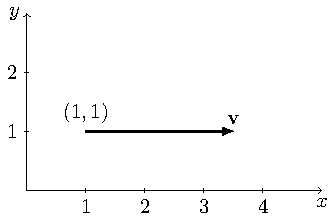
\includegraphics{vectorBaseAtPointOfAction}
\caption{سمتیہ}
\label{شکل_سمتیہ_دم_پر_عمل_درآمد_ہوتی_ہے}
\end{figure}

\حصہ{سمتی الجبرا}
دو سمتیوں کا ترسیمی  مجموعہ حاصل کرنے کی خاطر ایک سمتیہ کے سر کو دوسری سمتیہ کے دُم  کے ساتھ ملایا جاتا ہے۔پہلی سمتیہ کی دُم سے دوسری سمتیہ کے سر تک سمتیہ حاصل جمع ہو گا۔اس عمل کو شکل \حوالہ{شکل_سمتیہ_سمتیوں_کا_مجموعہ}-الف میں دکھایا گیا ہے۔شکل میں \سمتیہ{A} کے سر کے ساتھ \سمتیہ{B} کی دُم ملائی گئی ہے۔دو سے زیادہ سمتیوں کا مجموعہ بھی اسی عمل کو استعمال کرتے  ہوئے حاصل کیا جاتا ہے۔اس عمل کو \اصطلاح{سر سے دُم جوڑنا}\فرہنگ{سر سے دُم جوڑنا}\فرہنگ{head to tail rule}\حاشیہب{head to tail rule} کہتے ہیں۔شکل \حوالہ{شکل_سمتیہ_سمتیوں_کا_مجموعہ}-ب میں دو سمتیوں کے دُم ملا کر سمتیوں کے متوازی الاضلاع\فرہنگ{متوازی الاضلاع}\حاشیہب{parallelogram law}\فرہنگ{parallelogram law}  سے ان کا مجموعہ حاصل کرنا دکھایا گیا ہے جسے دیکھ کر صاف ظاہر ہے کہ $\bf{A}+\bf{B}=\bf{B}+\bf{A}$ ہے یعنی سمتیوں کا مجموعہ قانون تبادل\فرہنگ{قانون تبادل}\حاشیہب{commutative law}\فرہنگ{commutative law} پر پورا اترتا ہے۔اسی طرح سمتیوں کا مجموعہ قانون تلازمی\فرہنگ{قانون تلازمی}\حاشیہب{associative law}\فرہنگ{associative law}
\begin{align}
\bf{A}+\left(\bf{B}+\bf{C}\right)=\left(\bf{A}+\bf{B}\right)+\bf{C}
\end{align}
 پر بھی پورا اترتا ہے۔
%  
\begin{figure}
\begin{subfigure}{0.4\textwidth}
\centering
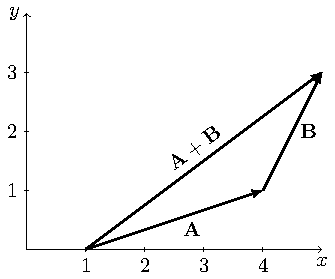
\includegraphics{figVectorHeadToTailRule}
\caption{سر کے ساتھ دُم جوڑ کر مجموعہ حاصل کیا جاتا ہے۔}
%\label{شکل_سمتیہ_سر_دم_جوڑنا}
\end{subfigure}
%
\begin{subfigure}{0.4\textwidth}
\centering
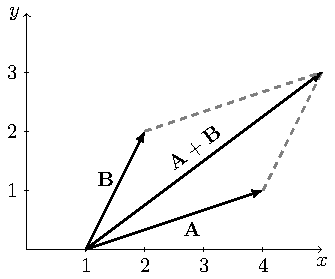
\includegraphics{figVectorParallelogramAdditionLaw}
\caption{متوازی الاضلاع سے بھی مجموعہ حاصل کیا جاتا ہے۔}
%\label{شکل_سمتیہ_متوازی_الاضلاع}
\end{subfigure}
\caption{سمتیوں کے مجموعے کا حصول}
\label{شکل_سمتیہ_سمتیوں_کا_مجموعہ}
\end{figure}

سمتیوں کے تفریق کا اصول  جمع کے اصول سے حاصل کیا جا سکتا ہے۔ہم $\bf{A}-\bf{B}$ کو $\bf{A}+\left(-\bf{B}\right)$ لکھ سکتے ہیں جہاں $-\bf{B}$ سے مراد یہ ہے کہ سمتیہ $\bf{B}$ کی سمت الٹی کر دی گئی ہے۔یوں $\bf{A}-\bf{B}$ حاصل کرنے کی خاطر $\bf{B}$ کی سمت الٹی کرتے ہوئے اس نئے سمتیہ کو $\bf{A}$ کے ساتھ جمع کیا جاتا ہے۔

سمتیہ \سمتیہ{A} کو مثبت  مقداری \عددیء{k} سے ضرب دینے سے سمتیہ کی سمت پر کوئی اثر نہیں ہوتا جبکہ اس کی لمبائی \عددیء{k} گنا ہو جاتی ہے۔اس کے برعکس سمتیہ \سمتیہ{A} کو منفی مقداری \عددیء{-k} سے ضرب دینے سے سمتیہ کی سمت الٹ ہو جاتی ہے اور اس کی لمبائی \عددیء{\abs{k}} گنا ہو جاتی ہے۔

دو سمتیے اُس صورت میں برابر ہوتے ہیں جب ان کا تفریق صفر کے برابر ہو یعنی \عددیء{\kvec{A}=\kvec{B}} تب ہو گا جب \عددیء{\kvec{A}-\kvec{B}=0} ہو۔

سمتی میدان کے متغیرات کو ہم آپس میں جمع یا منفی صرف اُس صورت کریں گے جب یہ متغیرات ایک ہی نقطے پر بیان کئے گئے ہوں۔یوں کسی بھی نقطے پر دو یا دو سے زیادہ مقناطیسوں کا اجتماعی مقناطیسی میدان حاصل کرتے ہوئے اس نقطے پر تمام مقناطیسوں کا علیحدہ علیحدہ مقناطیسی میدان لیتے ہوئے ان کا مجموعہ لیا جائے گا۔

اگر سمتی میدان کی بات نہ ہو رہی ہو تب مختلف مقامات پر پائے جانے والے سمتیوں کا بھی مجموعہ یا فرق لیا جا سکتا ہے۔یوں سمندر کے پانی میں ڈوبے  آب دوز کی اوپر اور نچلی سطح پر قوت کا مجموعہ حاصل کرتے ہوئے ہم یہ معلوم کر سکتے ہیں کہ آیا یہ مزید ڈوبے گا یا نہیں۔  

\حصہ{کارتیسی محدد}\شناخت{حصہ_سمتیہ_کارتیسی_محدد}
ایسا طریقہ جس سے کسی نقطے کا مقام بیان کیا جائے محدد\فرہنگ{محدد}\حاشیہب{coordinates}\فرہنگ{coordinates} کہلاتا ہے۔سیدھی سطح پر کسی بھی نقطے کو دو محدد سے ظاہر کیا جا سکتا ہے۔خلاء تین طرفہ\حاشیہب{three dimensional} ہے لہٰذا خلاء میں کسی بھی نقطے کو تین محدد سے ظاہر کیا جا سکتا ہے۔شکل \حوالہ{شکل_سمتیہ_اکائی_سے_سمتیہ_کا_اظہار}-الف میں دو طرفہ  \اصطلاح{کارتیسی} محدد پر اکائی لمبائی کے دو سمتیات \عددیء{\ax} اور \عددیء{\ay} دکھائے گئے ہیں۔اکائی سمتیہ \عددیء{\ax} کی سمت مثبت \عددیء{x} جانب کو ہے جبکہ \عددیء{\ay}  کی سمت مثبت \عددیء{y} جانب کو ہے۔شکل-ب میں \سمتیہ{A} دکھایا گیا ہے۔کسی بھی سمتیہ کو دو یا دو سے زیادہ سمتیوں کے مجموعے کی شکل میں لکھا جا سکتا ہے۔شکل میں \عددیء{\kvec{A}} کو \عددیء{\kvec{A}_x} اور \عددیء{\kvec{A}_y} کے مجموعے کی شکل میں دکھایا گیا ہے یعنی
\begin{align}
\kvec{A}=\kvec{A}_x+\kvec{A}_y
\end{align}

\begin{figure}
\begin{subfigure}{0.5\textwidth}
\centering
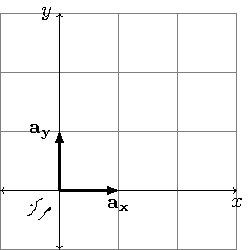
\includegraphics{unitVectorsInTwoDimensionalCartesianSpace}
\caption{اکائی سمتیہ}
%\label{شکل_سمتیہ_سر_دم_جوڑنا}
\end{subfigure}
%
\begin{subfigure}{0.5\textwidth}
\centering
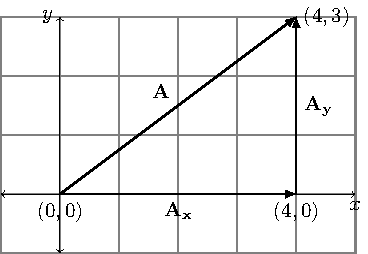
\includegraphics{vectorsRepresentationCartesianSpace}
\caption{اکائی سمتیات سے عمومی سمتیہ کا اظہار۔}
%\label{شکل_سمتیہ_متوازی_الاضلاع}
\end{subfigure}
\caption{اکائی سمتیات اور ان کا استعمال}
\label{شکل_سمتیہ_اکائی_سے_سمتیہ_کا_اظہار}
\end{figure}
%


زمین کی سطح کو لامحدود سیدھی سطح تصور کرتے ہوئے،  اس کے \اصطلاح{ہم سطحی}\فرہنگ{ہم سطحی}\حاشیہب{coplanar}\فرہنگ{coplanar} دو عمودی لکیریں کھینچتے ہوئے ایک لکیر کو \عددیء{x} محدد اور دوسری لکیر کو \عددیء{y} محدد تصور کیا جا سکتا ہے۔زمین کے ہم سطحی لکیر سے مراد ایسی لکیر ہے جس پر ہر نقطہ اس سطح کو چھوتا ہے۔\عددیء{x} محدد کے مثبت حصے  سے گھڑی کی الٹ سمت گھومتے ہوئے نوے درجے پر \عددیء{y} محدد کا مثبت حصہ رکھتے ہوئے اونچائی کو \عددیء{z} محدد کے مثبت حصے  سے ظاہر کیا جائے گا۔ اب اگر اونچائی صفر رکھتے ہوئے \عددیء{x} اور \عددیء{y} کو تبدیل کیا جائے تو ہم زمین کی سطح پر حرکت کریں گے۔اس طرح ہم دیکھتے ہیں کہ زمین کی سطح پر \عددیء{z=0} جبکہ اس پر \عددیء{x} اور \عددیء{y} آزاد متغیرات ہیں۔یوں زمین کی سطح کو \عددیء{z=0} سطح کہتے ہیں جسے
\begin{align*}
z=0, \quad  x\le \abs{\mp \infty}, \quad y \le \abs{\mp \infty}
\end{align*} 
لکھا جا سکتا ہے۔  شکل \حوالہ{شکل_سمتیہ_کارتیسی_نقطہ_اور_عمودی_سطحیں}-الف میں اس سطح کی نشاندہی کی گئی ہے۔ہم بالکل اسی طرح \عددیء{y=0} سطح اور \عددیء{x=0} سطح بھی بیان کر سکتے ہیں۔

\begin{figure}
\begin{subfigure}{0.4\textwidth}
\centering
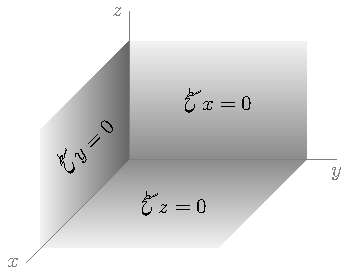
\includegraphics{figVectorPlaneSurfacesCartesian}
\caption{کارتیسی محدد میں عمودی سیدھی سطحیں۔}
\label{شکل_سمتیہ_کارتیسی_عمودی-تین_سطحیں}
\end{subfigure}%
%
\begin{subfigure}{0.4\textwidth}
\centering
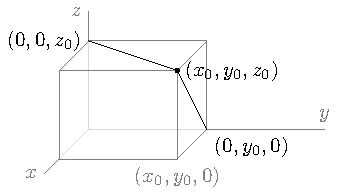
\includegraphics{figVectorPerpendicularsFromPointToCartesianAxis3D}
\caption{نقطے سے محدد پر عمود۔}
\label{شکل_سمتیہ_نقطے_سے_کارتیسی_محدد_پر_عمود}
\end{subfigure}%
\caption{کارتیسی نظام میں نقطہ اور تین عمودی سطحیں۔}
\label{شکل_سمتیہ_کارتیسی_نقطہ_اور_عمودی_سطحیں}
\end{figure}
شکل  \حوالہ{شکل_سمتیہ_کارتیسی_نقطہ_اور_عمودی_سطحیں}-ب  کو دیکھتے ہوئے آگے  پڑھیں۔ کارتیسی محدد میں کسی بھی نقطے کو \عددیء{(x_0,y_0,z_0)} لکھا جا سکتا ہے۔اس نقطے تک پہنچنے کی خاطر  کارتیسی محدد کے مرکز سے پہلے \عددیء{x} محدد کے متوازی \عددیء{x_0}  فاصلہ طے کرتے ہوئے \عددیء{(x_0,0,0)} تک پہنچیں۔اس کے بعد \عددیء{y} محدد کے متوازی \عددیء{y_0} فاصلہ طے کرتے ہوئے \عددیء{(x_0,y_0,0)} تک پہنچیں  اور آخرکار \عددیء{z} محدد کے متوازی \عددیء{z_0} فاصلہ طے کرتے ہوئے درکار نقطہ \عددیء{(x_0,y_0,z_0)} تک پہنچیں۔اس عمل میں یہ ضروری نہیں کہ پہلے \عددیء{x} محدد کے متوازی ہی چلا جائے۔آپ مرکز سے پہلے \عددیء{y} محدد کے متوازی \عددیء{y_0} فاصلہ طے کرنے کے بعد \عددیء{z} محدد کے متوازی \عددیء{z_0} اور آخرکار \عددیء{x} محدد کے متوازی \عددیء{x_0} فاصلہ طے کرتے ہوئے بھی اسی نقطے تک پہنچ سکتے ہیں۔تینوں فاصلوں کو کسی بھی ترتیب سے طے کیا جا سکتا ہے۔

 نقطہ \عددیء{(x_0,y_0,z_0)} سے \عددیء{x} محدد پر عمود بناتے ہوئے  \عددیء{(x_0,0,0)} حاصل ہوتا ہے۔اسی طرح اس نقطے سے \عددیء{y} محدد پر عمود \عددیء{(0,y_0,0)} اور \عددیء{z} محدد پر عمود \عددیء{(0,0,z_0)} دیتا ہے۔نقطہ \عددیء{(x_0,y_0,z_0)} سے \عددیء{y} محدد اور \عددیء{z} محدد پر عمودی لکیریں گہری سیاہی میں دکھائے گئے ہیں۔ اگر \عددیء{(x_0,y_0,z_0)} سے  شروع ہوتے ہوئے \عددیء{z} محدد کے متوازی یوں چلا جائے کہ آخرکار \عددیء{z=0} ہو جائے تو نقطہ \عددیء{(x_0,y_0,0)} حاصل ہو گا۔ اب اگر یہاں سے \عددیء{x} محدد کے متوازی یوں چلا جائے کہ آخرکار \عددیء{x=0} ہو جائے تو نقطہ \عددیء{(0,y_0,0)} حاصل ہو گا۔یہ وہی نقطہ ہے جو \عددیء{(x_0,y_0,z_0)} سے \عددیء{y} محدد پر عمودی لکیر بناتے ہوئے حاصل ہوتا ہے۔اس عمل میں ہم پہلے \عددیء{x} محدد کے متوازی چلتے ہوئے \عددیء{x=0} کرنے کے بعد \عددیء{z} محدد کے متوازی چلتے ہوئے \عددیء{z=0} کرتے ہوئے بھی نقطہ \عددیء{(0,y_0,0)} تک پہنچ سکتے تھے۔

نقطہ \عددیء{(x_0,y_0,z_0)} تک قدر مختلف انداز سے بھی پہنچا جا سکتا ہے جسے کارتیسی محدد میں سمجھنا زیادہ آسان ہے۔فرض کریں کہ \عددیء{x=x_0} پر لامحدود \عددیء{yz} سیدھی سطح بنائی جائے۔ایسی سطح کو \عددیء{x=x_0} سطح  کہتے ہیں۔اس سطح کو
\begin{align*}
x=x_0, \quad  y\le \abs{\mp \infty}, \quad z \le \abs{\mp \infty}
\end{align*} 
لکھا جا سکتا ہے۔اس مساوات میں \عددیء{x_0} مقررہ ہے جبکہ \عددیء{y} اور \عددیء{z} متغیرات ہیں۔دو متغیرات کی مساوات سطح کو ظاہر کرتی ہے۔اگر \عددیء{y=y_0} پر لامحدود \عددیء{xz} سیدھی سطح بنائی جائے تو یہ دو سطحے  آپس میں سیدھی لکیر پر ملیں گے۔یہ لکیر
\begin{align*}
x=x_0, \quad  y=y_0, \quad z \le \abs{\mp \infty}
\end{align*} 
لکھی جا سکتی ہے۔اس مساوات میں \عددیء{x_0} اور \عددیء{y_0} مقررہ ہیں جبکہ \عددیء{z} متغیرہ ہے۔ایک متغیرہ کی مساوات لکیر کو ظاہر کرتی ہے۔اب اگر \عددیء{z=z_0} پر لامحدود \عددیء{xy} سیدھی سطح بھی بنائی جائے تب یہ تینوں سطحے ایک نقطے \عددیء{N(x_0,y_0,z_0)} پر آپس کو چھوئنگے۔یہ صورت حال شکل \حوالہ{شکل_سمتیہ_تین_عمودی_سطحوں_سے_نقطہ} میں دکھائی گئی ہے جہاں لامحدود سطحوں کے کچھ حصے دکھائے گئے ہیں۔آپ دیکھیں گے کہ نقطے تک پہنچنے کا یہ طریقہ دیگر محدد میں استعمال کرنا لازمی ثابت ہو گا۔
\begin{figure}
\centering
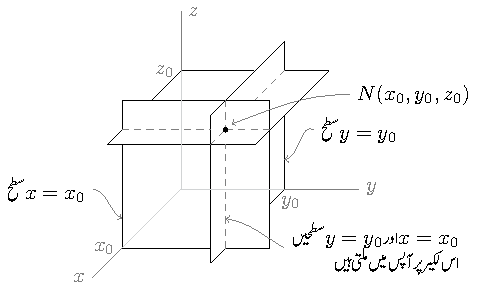
\includegraphics{figVectorLineAsSurfacesTouching}
\caption{تین عمودی سطحوں سے نقطے کا حصول۔}
\label{شکل_سمتیہ_تین_عمودی_سطحوں_سے_نقطہ}
\end{figure}

اگر سطح \عددیء{x=x_0}  کے متوازی \عددیء{x=x_0+\dif x} پر اور اسی طرح \عددیء{y=y_0} کے متوازی \عددیء{y=y_0+\dif y} اور \عددیء{z=z_0} کے متوازی \عددیء{z=z_0+\dif z} سطح رکھے جائیں تو یہ چھ سطحے ایک چھوٹی  مکعب نما حجم  کو گھیریں گی جسے شکل \حوالہ{شکل_سمتیہ_کارتیسی_چھوٹی_مکعب} میں دکھایا گیا ہے جبکہ یہ تین نئی سطحیں آپس میں نقطہ \عددیء{N'} پر ملیں گی ۔
\begin{figure}
\centering
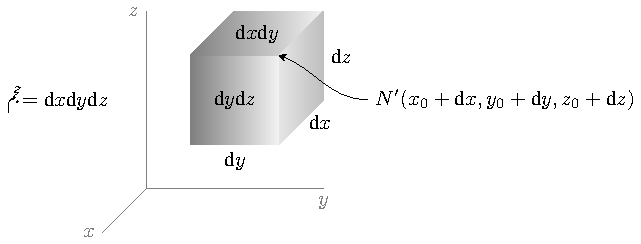
\includegraphics{figVectorCubeShaded}
\caption{چھ سطحے مکعب گھیرتی ہیں۔}
\label{شکل_سمتیہ_کارتیسی_چھوٹی_مکعب}
\end{figure}
اس مکعب نما کے اطراف \عددیء{\dif x}، \عددیء{\dif y} اور \عددیء{\dif z} ہیں۔ اس کی اوپر والی سطح کا رقبہ \عددیء{\dif x \dif y} ہے۔اسی طرح اس کی نچلی سطح کا رقبہ بھی \عددیء{\dif x \dif y} ہے۔سامنے سطح  اور پچھلی سطح دونوں \عددیء{\dif y \dif z} رقبے رکھتے ہیں جبکہ بائیں  اور دائیں سطحوں کے رقبے \عددیء{\dif x \dif z} کے برابر ہیں۔اس مکعب نما کی حجم \عددیء{\dif x \dif y \dif z} ہے۔نقطہ \عددیء{N'(x_0+\dif x,y_0+\dif y,z_0+\dif z)} شکل میں دکھایا گیا ہے جبکہ
 نقطہ \عددیء{N(x_0,y_0 ,z_0)} مکعب نما کا وہ واحد کونا ہے جسے شکل میں نہیں دکھایا گیا۔ان دو نقطوں کے درمیان فاصلہ \عددیء{NN'=\sqrt{\dif x^2+\dif y^2+\dif z^2}} ہے۔ 

کارتیسی محدد کے تینوں متغیرات تبدیل کرنے سے ہم \عددیء{N} سے \عددیء{N'} پہنچتے ہیں۔\عددیء{N} سے \عددیء{N'} تک کی سمتیہ

\begin{align}\label{مساوات_سمتیہ_کارتیسی_چھوٹا_فاصلہ}
\dif \kvec{L}=\dif x \ax+\dif y \ay+\dif z \az
\end{align}
لکھی جاتی ہے۔یہ مساوات کسی بھی دو قریبی نقطوں کے درمیان سمتی لمبائی دیتی ہے۔
%==================
\حصہ{اکائی سمتیات}
حصہ  \حوالہ{حصہ_سمتیہ_کارتیسی_محدد} کے شروع میں دو طرفہ کارتیسی نظام  میں سیدھی سطح پر کسی بھی سمتیہ کو دو سمتیات کی صورت میں لکھنا دکھایا گیا۔یہی طریقہ تین طرفہ کارتیسی نظام کے لئے بھی استعمال کیا جاتا ہے۔ تین طرفہ کارتیسی نظام کے تین اکائی سمتیات \عددیء{\ax}، \عددیء{\ay} اور \عددیء{\az} لکھے جاتے ہیں۔یہ تینوں سمتیات آپس میں عمودی ہیں۔کسی بھی اکائی سمتیہ کی طرح یہ تین اکائی سمتیات اکائی لمبائی رکھتے ہیں۔ \عددیء{\ax} کی سمت \عددیء{x} محدد کے بڑھتے جانب کو ہے۔اسی طرح \عددیء{\ay} کی سمت \عددیء{y} محدد کے بڑھتے جانب کو اور \عددیء{\az} کی سمت \عددیء{z} محدد کے بڑھتے جانب کو ہے۔شکل \حوالہ{شکل_سمتیہ_کارتیسی_تین_اکائی_سمتیات}-الف میں یہ تینوں اکائی سمتیات دکھائے گئے ہیں۔اسی شکل میں نقطہ \عددیء{(0,1,2)} پر سمتیہ دکھایا گیا ہے جس کی لمبائی دو کے برابر ہے جبکہ یہ اکائی سمتیہ \عددیء{\ay} کی سمت میں ہے۔اس سمتیہ کو \عددیء{2\ay} لکھا جا سکتا ہے۔یاد رہے کہ ایسے دو سمتیات برابر ہوتے ہیں جن کا طول برابر ہو اور جو ایک ہی سمت میں ہوں۔ یوں سمت تبدیل کئے بغیر سمتیہ کو کارتیسی محدد کے مرکز منتقل کرتے ہوئے اس کی قیمت نسبتاً آسانی سے لکھی جا سکتی ہے۔
\begin{figure}
\centering
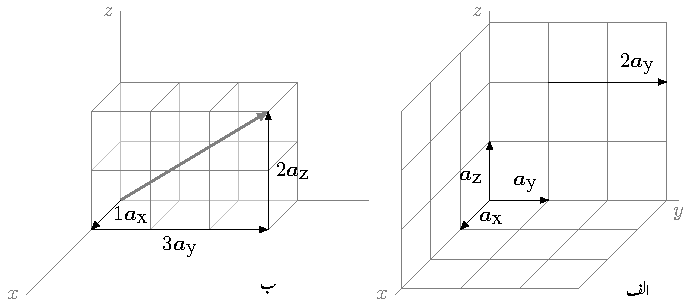
\includegraphics{figVector3DUnitVectors}
\caption{کارتیسی نظام کے اکائی سمتیات اور ان کا استعمال}
\label{شکل_سمتیہ_کارتیسی_تین_اکائی_سمتیات}
\end{figure}
%
\begin{figure}
\centering
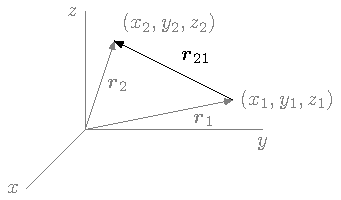
\includegraphics{figVector3DcartesianVectorEquation}
\caption{کارتیسی نظام میں سمتیہ کی مساوات کا حصول}
\label{شکل_سمتیہ_کارتیسی_سمتیہ_کی_مساوات}
\end{figure}
%
\begin{figure}
\centering
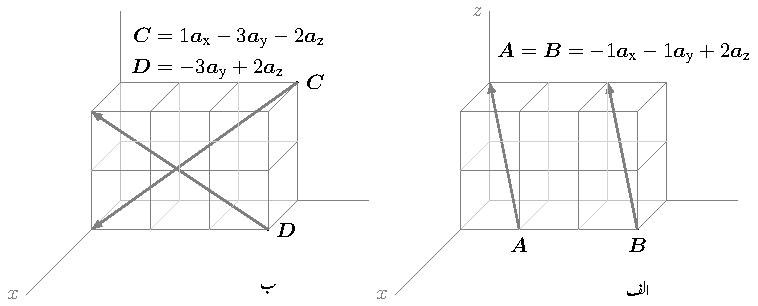
\includegraphics{figVector3DcartesianVectors}
\caption{کارتیسی نظام میں چند سمتیات۔}
\label{شکل_سمتیہ_کارتیسی_چند_سمتیات}
\end{figure}
%

شکل \حوالہ{شکل_سمتیہ_کارتیسی_سمتیہ_کی_مساوات} میں  مرکز سے \عددیء{(x_1,y_1,z_1)} تک سمتیہ \عددیء{\kvec{r}_1=x_1 \ax+y_1\ay+z_1\az} اور  مرکز سے \عددیء{(x_2,y_2,z_2)} تک سمتیہ \عددیء{\kvec{r}_2=x_2 \ax+y_2\ay+z_2\az} دکھائے گئے ہیں۔شکل میں سمتیہ \عددیء{\kvec{r}_{21}} بھی دکھائی گئی ہے جس کی دُم  \عددیء{(x_1,y_1,z_1)} اور  نوک \عددیء{(x_2,y_2,z_2)} پر ہے۔ سر سے دُم جوڑنے کے اصول کے استعمال سے \عددیء{\kvec{r}_2=\kvec{r}_{21}+\kvec{r}_1} لکھا جا سکتا ہے جس سے 
\begin{gather}
\begin{aligned}\label{مساوات_سمتیہ_کارتیسی_نظام_میں_قیمت}
\kvec{r}_{21}&=\kvec{r}_2-\kvec{r}_1\\
&=(x_2-x_1) \ax+(y_2-y_1)\ay+(z_2-z_1)\az
\end{aligned}
\end{gather}
حاصل ہوتا ہے۔اس مساوات کے استعمال سے سمتیہ کی مساوات باآسانی حاصل ہوتی ہے۔سمتیہ \عددیء{\kvec{r}_{21}} لکھتے ہوئے زیرنوشت میں سمتیہ کی نوک کو \عددیء{2} اور اس کی دُم  کو \عددیء{1} سے ظاہر کیا گیا ہے۔اس کتاب میں سمتیہ لکھتے ہوئے نوک اور دُم  کو اسی ترتیب سے زیرنوشت میں لکھا جائے گا۔یوں سمتیہ \عددیء{\kvec{r}_{21}} کو تین اجزاء \عددیء{(x_2-x_1)\ax}، \عددیء{(y_2-y_1)\ay} اور \عددیء{(z_2-z_1)\az} کے  مجموعے کی شکل میں لکھا جا سکتا ہے۔

شکل \حوالہ{شکل_سمتیہ_کارتیسی_تین_اکائی_سمتیات}-ب میں مرکز سے \عددیء{(1,3,2)} تک سمتیہ دکھایا گیا ہے۔آپ دیکھ سکتے ہیں کہ اس کو تین سمتیات کا مجموعہ لکھا جا سکتا ہے یعنی \عددیء{1\ax+3\ay+2\az} جہاں اکائی سمتیات استعمال کرتے ہوئے تینوں اجزاء کو لکھا گیا ہے۔ سمتیہ کی دُم \عددیء{(0,0,0)} اور اس کی نوک \عددیء{(1,3,2)} پر لیتے ہوئے  یہی جواب  مساوات \حوالہ{مساوات_سمتیہ_کارتیسی_نظام_میں_قیمت} سے بھی حاصل ہوتا ہے۔

شکل \حوالہ{شکل_سمتیہ_کارتیسی_چند_سمتیات}-الف میں دو متوازی سمتیات \عددیء{\kvec{A}} اور \عددیء{\kvec{B}} دکھائے ہیں جن کی لمبائی برابر ہے۔ چونکہ ان کی لمبائی برابر ہے اور یہ دونوں ایک ہی سمت میں ہیں لہٰذا \عددیء{\kvec{A}=\kvec{B}=-1\ax-1\ay+2\az} لکھا جائے گا۔شکل \حوالہ{شکل_سمتیہ_کارتیسی_چند_سمتیات}-ب میں \عددیء{\kvec{C}} کی دُم سے \عددیء{\ax} جانب ایک قدم اور یہاں سے \عددیء{-\ay} جانب تین قدم اور آخرکار \عددیء{-\az} جانب دو قدم چلنے سے اس کی نوک تک پہنچا جا سکتا ہے لہٰذا \عددیء{\kvec{C}=1\ax-3\ay-2\az} لکھا جائے گا۔ اسی طرح \عددیء{\kvec{D}} کی دُم سے  \عددیء{-\ay} جانب تین قدم اور پھر \عددیء{\az} جانب دو قدم چلتے ہوئےسمتیہ کی نوک تک پہنچا جایا سکتا ہے لہٰذا \عددیء{\kvec{D}=-3\ay+2\az} لکھا جائے گا۔سمتیہ \عددیء{\kvec{D}} کو دو اجزاء کی شکل میں لکھا گیا ہے چونکہ اس کے تیسرے جزو کی لمبائی صفر کے برابر ہے۔
%=====================
\ابتدا{مشق}
مساوات \حوالہ{مساوات_سمتیہ_کارتیسی_نظام_میں_قیمت} کے استعمال سے شکل \حوالہ{شکل_سمتیہ_کارتیسی_چند_سمتیات} میں تمام سمتیات لکھیں۔

جوابات:تمام جوابات شکل میں دئے گئے ہیں۔
\انتہا{مشق}
%======================
\begin{figure}
\centering
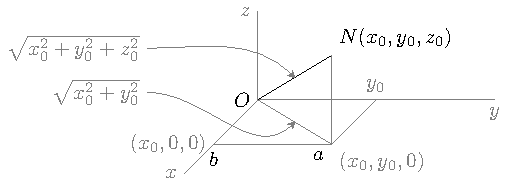
\includegraphics{figVectorCartesianAmplitudeFromPythagorousTheorem}
\caption{کارتیسی نظام میں سمتیہ کا طول۔}
\label{شکل_سمتیہ_کارتیسی_سمتیہ_طول}
\end{figure}

شکل \حوالہ{شکل_سمتیہ_کارتیسی_سمتیہ_طول} میں مرکز سے نقطہ \عددیء{N(x_0,y_0,z_0)} تک کا فاصلہ \عددیء{ON} مسئلہ \اصطلاح{فیثاغورث}\فرہنگ{فیثاغورث}\حاشیہب{Pythagoras theorem}\فرہنگ{Pythagoras theorem} سے حاصل کیا جا سکتا ہے۔اس نقطے سے \عددیء{z=0} سطح پر عمود سے نقطہ \عددیء{a} حاصل ہوتا ہے۔نقطہ \عددیء{a} سے \عددیء{x} محدد پر عمود نقطہ \عددیء{b} دیتا ہے۔تکون \عددیء{Oba} میں \عددیء{O} سے \عددیء{b} کا فاصلہ \عددیء{x_0} ہے جبکہ \عددیء{b} سے \عددیء{a} کا فاصلہ \عددیء{y_0} ہے۔یوں فاصلہ \عددیء{Oa} مسئلہ فیثاغورث کی مدد سے  \عددیء{\sqrt{x_0^2+y_0^2}} کے برابر ہو گا۔ تکون \عددیء{OaN} میں \عددیء{a} پر \عددیء{90^{\circ}} کا زاویہ پایا جاتا ہے۔یوں مسئلہ فیثاغورث کی مدد سے \عددیء{ON} کا فاصلہ \عددیء{\sqrt{x_0^2+y_0^2+z_0^2}} حاصل ہوتا ہے۔

مساوات \حوالہ{مساوات_سمتیہ_کارتیسی_نظام_میں_قیمت} سمتیہ کی عمومی مساوات ہے۔اس میں دئے سمتیہ \عددیء{\kvec{r}_{21}} کی دُم محدد کے مرکز پر رکھنے سے صاف ظاہر ہے کہ سمتیہ کی مقدار
\begin{align}
\abs{\kvec{r}_{21}}=r_{21}=\sqrt{(x_2-x_1)^2+(y_2-y_1)^2+(z_2-z_1)^2}
\end{align}
کے برابر ہے۔اگر سمتیہ کو اس کی مقدار سے تقسیم کیا جائے تو حاصل جواب کی مقدار اکائی ہو گی جبکہ اس کی سمت میں کوئی تبدیلی رونما نہیں ہو گی۔یوں  \عددیء{\kvec{r}_{21}} کو \عددیء{\abs{\kvec{r}_{21}}} سے تقسیم کرتے ہوئے \عددیء{\kvec{r}_{21}} کی سمت میں اکائی سمتیہ \عددیء{\kvec{a}_{r21}} حاصل کی جا سکتی ہے۔
\begin{align}
\kvec{a}_{r21}=\frac{\kvec{r}_{21}}{\abs{\kvec{r}_{21}}}=\frac{(x_2-x_1) \ax+(y_2-y_1)\ay+(z_2-z_1)\az}{\sqrt{(x_2-x_1)^2+(y_2-y_1)^2+(z_2-z_1)^2}}
\end{align}
یاد رہے کہ سمتیہ کی سمت اور طول تبدیل کئے بغیر اسے ایک مقام سے دوسری مقام منتقل کیا جا سکتا ہے۔البتہ وہ سمتیہ جو کسی نقطے کی مقام تعین کرتا ہو کو اگر کہیں اور منتقل کیا جائے تو ایسی صورت میں  سمتیہ کی نوک درکار نقطے پر نہیں رہے گی۔اسی حقیقت کی بنا پر میدان ظاہر کرنے والے سمتیہ کو اپنی جگہ سے نہیں ہٹایا جا سکتا۔میدانی سمتیہ کی دُم اس مقام پر پائی جاتی ہے جہاں میدان بیان کی جا رہی ہو۔  

سمتیات کے استعمال سے نقطہ \عددیء{(x,y,z)} کے مقام کو \عددیء{\kvec{r}=x\ax+y\ay+z\az} لکھا جاتا ہے۔کسی بھی سمتیہ مثلاً قوت \عددیء{\kvec{F}} کو بالکل اسی طرح  \عددیء{{\kvec{F}=F_x\ax+F_y\ay+F_z\az}} لکھا جاتا ہے جہاں \عددیء{F_x \ax}، \عددیء{F_y \ay} اور \عددیء{F_z\az} اس کے تین اجزاء اور
  \عددیء{\abs{\kvec{F}}=\sqrt{F_x^2+F_y^2+F_z^2}} قوت کی مقدار ہے۔
%======================
\ابتدا{مثال}
نقطہ \عددیء{(-5,2,-1)}  کا مقام ظاہر کرنے والا سمتیہ اور اس سمتیہ کا طول حاصل کریں۔اسی سمتیہ کی سمت میں اکائی سمتیہ حاصل کریں۔

حل:مرکز سے اس نقطے تک کا سمتیہ \عددیء{\kvec{r}=-5\ax+2\ay-1\az} ہے جبکہ اس سمتیہ  کا طول \عددیء{\abs{\kvec{r}}=\sqrt{5^2+2^2+1^1}=\sqrt{30}} ہے۔یوں اکائی سمتیہ \عددیء{\kvec{a}_r=\tfrac{-5\ax+2\ay-1\az}{\sqrt{30}}} ہو گا۔
\انتہا{مثال}
%=====================

\ابتدا{مثال}\شناخت{مثال_سمتیہ_نقطے_سے_درمیان_تک_سمتیہ}
شکل \حوالہ{شکل_سمتیہ_استعمال_سمتیہ_مثال} میں تین نقطے \عددیء{M(1,6,4)}، \عددیء{N(4,5,1)} اور \عددیء{P(1,2,2)} دئے گئے ہیں۔\عددیء{M} اور \عددیء{N} کے درمیان سیدھی لکیر پر \عددیء{M} سے کل فاصلے کے  \عددیء{\tfrac{1}{3}} پر نقطہ \عددیء{Q} پایا جاتا ہے۔\عددیء{Q} سے \عددیء{P} تک سمتیہ حاصل کرتے ہوئے ان دو نقطوں کے درمیان فاصلہ معلوم کریں۔
\begin{figure}
\centering
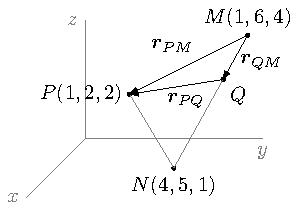
\includegraphics{figVectorExampleA}
\caption{سمتیوں کا استعمال}
\label{شکل_سمتیہ_استعمال_سمتیہ_مثال}
\end{figure}
حل:\عددیء{M} سے \عددیء{N} تک سمتیہ
\begin{align*}
\kvec{r}_{NM}&=(4-1)\ax+(5-6)\ay+(1-4)\az\\
&=3\ax-1\ay-3\az
\end{align*}
ہے۔\عددیء{M} سے \عددیء{Q} تک سمتیہ \عددیء{\kvec{r}_{QM}} اور \عددیء{\kvec{r}_{NM}} ایک ہی سمت میں ہیں جبکہ \عددیء{\abs{\kvec{r}_{QM}}=\tfrac{1}{3}\abs{\kvec{r}_{NM}}} کے برابر ہے۔یوں
\begin{align*}
\kvec{r}_{QM}=\frac{1}{3}\kvec{r}_{NM}=\frac{1}{3}(3\ax-1\ay-3\az)=1\ax-\frac{1}{3}\ay-1\az
\end{align*}
ہو گا۔\عددیء{M} سے \عددیء{P} تک سمتیہ
\begin{align*}
\kvec{r}_{PM}&=(1-1)\ax+(2-6)\ay+(2-4)\az\\
&=-4\ay-2\az
\end{align*}
ہے۔شکل کو دیکھتے ہوئے ہم لکھ سکتے ہیں \عددیء{\kvec{r}_{QM}+\kvec{r}_{PQ}=\kvec{r}_{PM}} لہٰذا
\begin{align*}
\kvec{r}_{PQ}&=\kvec{r}_{PM}-\kvec{r}_{QM}\\
&=(-4\ay-2\az)-(1\ax-\frac{1}{3}\ay-1\az)\\
&=-1\ax-\frac{11}{3}\ay-1\az
\end{align*}
ہو گا۔\عددیء{Q} سے \عددیء{P} تک فاصلہ \عددیء{\sqrt{1^1+\left(\tfrac{11}{3}\right)^2+1^2}=3.93} ہے۔
\انتہا{مثال}
%===================
\ابتدا{مشق}
مثال \حوالہ{مثال_سمتیہ_نقطے_سے_درمیان_تک_سمتیہ} میں دئے نقطوں کو استعمال کرتے ہوئے \عددیء{M} سے \عددیء{P} تک سمتیہ حاصل کریں۔اسی طرح \عددیء{P} سے \عددیء{N} تک سمتیہ اور \عددیء{M} سے \عددیء{N} تک سمتیہ حاصل کریں۔پہلے دو جوابات کو استعمال کرتے ہوئے \اصطلاح{سر سے دُم جوڑنے} کے اصول سے تیسرا سمتیہ دوبارہ حاصل کریں۔

جوابات:\عددیء{-5\ax-4\ay} ، \عددیء{-1\ax+4\ay+12\az} اور \عددیء{-6\ax+12\az}

\انتہا{مشق}
%============================================


\حصہ{سمتی رقبہ}
کسی بھی سطح کے دو اطراف ہوتے ہیں۔یوں سطح کے کسی بھی نقطے پر دو آپس میں الٹ سمتوں میں عمود بنائے جا سکتے ہیں۔سیدھی سطح جس کا رقبہ \عددیء{S} ہو کے ایک طرف پر اکائی عمود \عددیء{\kvec{a}_N} اور دوسری طرف پر اکائی عمود \عددیء{-\kvec{a}_N} بنائے جا سکتے ہیں۔اگر ان دو عمود میں سے ایک عمود مثلاً \عددیء{\kvec{a}_N} کو سطح کی سمت\حاشیہد{عمود سطح کے ساتھ نوے درجہ زاویہ بناتا ہے۔\عددیء{\kvec{a}_N} کے زیرنوشت میں \عددیء{N}، لفظ \موٹا{نوے} کے پہلے حرف کی آواز کو ظاہر کرتا ہے۔} تصور کیا جائے تب اس سطح کا \اصطلاح{سمتی رقبہ}\فرہنگ{سمتی رقبہ}\حاشیہب{vector area}\فرہنگ{vector area} \عددیء{S\kvec{a}_N} ہو گا۔بند سطح کے  بیرونی اکائی عمود کو سطح کی سمت تصور کیا جاتا ہے۔شکل \حوالہ{شکل_سمتیہ_سمتی_رقبہ} میں سمتی رقبے \عددیء{\kvec{A}_1} اور \عددیء{\kvec{A}_2} دکھائے گئے ہیں جہاں بند سطح کے بیرونی عمود کو ہی سطح کی سمت دکھایا گیا ہے۔
\begin{figure}
\centering
\includegraphics{figVectorVectorArea}
\caption{سمتی رقبہ}
\label{شکل_سمتیہ_سمتی_رقبہ}
\end{figure}


\حصہ{غیر سمتی ضرب}
دو سمتیات \عددیء{\kvec{A}} اور \عددیء{\kvec{B}} کے \اصطلاح{غیر سمتی ضرب}\فرہنگ{غیر سمتی ضرب}\فرہنگ{نقطہ ضرب}\فرہنگ{مقداری ضرب}\حاشیہب{scalar product}\فرہنگ{scalar product} سے مراد \عددیء{\kvec{A}} کی مقدار ضربِ  \عددیء{\kvec{B}} کی مقدار ضربِ سمتیوں کے مابین چھوٹے زاویے کا کوسائن ہے۔
\begin{align}\label{مساوات_سمتیہ_مقداری_ضرب}
\kvec{A} \cdot \kvec{B}=\abs{\kvec{A}} \abs{\kvec{B}} \cos \theta_{AB}
\end{align}

اگر دونوں سمتیات کی دُم ایک ہی جگہ پر نہ ہو تب ان کے مابین زاویہ دریافت کرنے کی  خاطر سمتیوں کی سمت تبدیل کئے بغیر انہیں ایک نقطے پر منتقل کیا جا سکتا ہے۔غیر سمتی ضرب دو سمتیوں کے مابین کیا جاتا ہے جبکہ اس کا حاصل جواب مقداری ہوتا ہے جس کی وجہ سے اسے  \اصطلاح{مقداری ضرب} بھی کہا جاتا ہے۔غیر سمتی ضرب کو سمتیوں کے درمیان نقطے سے ظاہر کیا جاتا ہے۔اسی وجہ سے اسے \اصطلاح{ضرب نقطہ}\حاشیہب{dot product}\فرہنگ{dot product} بھی کہا جاتا ہے۔ یوں \عددیء{\kvec{A} \cdot \kvec{B}} کو "\عددیء{\kvec{A}}نقطہ \عددیء{\kvec{B}}" پڑھا جاتا ہے۔بالکل سادہ ضرب کی طرح \عددیء{\kvec{A} \cdot \kvec{B}} کو \عددیء{\kvec{B} \cdot \kvec{A}} بھی لکھا جا سکتا ہے یعنی غیر سمتی ضرب میں متغیرات کی ترتیب اہمیت نہیں رکھتی۔

کارتیسی اکائی سمتیات \عددیء{\ax}، \عددیء{\ay} اور \عددیء{\az} آپس میں عمودی ہیں لہٰذا ان میں کسی بھی دو سمتیات کے درمیان \عددیء{\SI{90}{\degree}} زاویہ پایا جاتا ہے۔چونکہ \عددیء{\cos 90=0} کے برابر ہوتا ہے لہٰذا ان میں کسی بھی دو سمتیوں کا غیر سمتی ضرب صفر کے برابر ہوتا ہے یعنی
\begin{align}\label{مساوات_سمتیہ_عمودی_نقطہ_ضرب_برابر_صفر_اجزاء}
\ax \cdot \ay =0, \quad \ax \cdot \az=0, \quad \ay \cdot \az=0
\end{align}
ایک ہی سمت میں دو سمتیوں کے درمیان صفر زاویہ ہوتا ہے اور \عددیء{\cos 0=1} کے برابر ہے۔ اکائی سمتیہ کا طول بھی ایک کے برابر ہے لہٰذا مساوات \حوالہ{مساوات_سمتیہ_مقداری_ضرب} کے تحت \عددیء{\ax} اور \عددیء{\ax} کا غیر سمتی ضرب
\begin{align*}
\ax \cdot \ax=(\abs{\ax})(\abs{\ax})(\cos 0\degree)=(1)(1)(1)=1
\end{align*}
ہو گا۔بقایا دو کارتیسی اکائی سمتیات کا خود غیر سمتی ضرب بھی ایک کے برابر ہے۔
\begin{align}\label{مساوات_سمتیہ_عمودی_نقطہ_ضرب_برابر_ایک_اجزاء}
\ax \cdot \ax=1, \quad \ay \cdot \ay=1, \quad \az \cdot \az=1
\end{align}
مساوات \حوالہ{مساوات_سمتیہ_عمودی_نقطہ_ضرب_برابر_صفر_اجزاء} اور مساوات \حوالہ{مساوات_سمتیہ_عمودی_نقطہ_ضرب_برابر_ایک_اجزاء} کو \اصطلاح{کرونیکر ڈیلٹا}\فرہنگ{کرونیکر ڈیلٹا}\حاشیہد{یہ لیوپولڈ کرونیکر کے نام سے  منسوب ہے۔} \عددیء{\delta_{ij}} کی مدد سے ایک ہی مساوات کی مدد سے یوں لکھا جا سکتا ہے۔
\begin{align}
\kvec{a}_i \cdot \kvec{a}_j=\delta_{ij}
\end{align}
جہاں
\begin{align}
\delta_{ij}=
\begin{cases}
0 \quad  \quad  i\ne j \; \textup{ اگر}\\
1 \quad \quad i=j \; \textup{ اگر}
\end{cases}
\end{align}
کے برابر ہے یعنی \عددیء{i=j} کی صورت میں ہی \عددیء{\delta_{ij}} کی قیمت ایک  جبکہ \عددیء{i\ne j} کی صورت میں ہی \عددیء{\delta_{ij}} کی قیمت صفر کے برابر لی جاتی ہے۔یوں \عددیء{\ax \cdot \ay} کی صورت میں \عددیء{i=\ax} جبکہ \عددیء{j=\ay} کے برابر ہیں۔یوں \عددیء{i} اور \عددیء{j} برابر نہیں ہیں لہٰذا حاصل جواب صفر کے برابر ہو گا۔اس کے برعکس \عددیء{\az \cdot \az} کی صورت میں \عددیء{i=\az} اور \عددیء{j=\az} ہیں لہٰذا \عددیء{i=j} ہے اور یوں حاصل جواب ایک کے برابر ہے۔

کارتیسی تین عمودی اکائیوں کی مدد سے سمتیات کا غیر سمتی ضرب نہایت آسانی سے حاصل ہوتا ہے۔یوں اگر \عددیء{\kvec{A}=A_x\ax+A_y\ay+A_z\az} اور  \عددیء{\kvec{B}=B_x\ax+B_y\ay+B_z\az}  دو سمتیات ہوں تب ان کا غیر سمتی ضرب
\begin{align*}
\kvec{A} \cdot \kvec{B}&=(A_x\ax+A_y\ay+A_z\az) \cdot (B_x\ax+B_y\ay+B_z\az)\\
&=A_x B_x \ax \cdot \ax+A_x B_y \ax \cdot \ay+A_x B_z \ax \cdot \az\\
& \quad \quad +A_y B_x \ay \cdot \ax+A_y B_y \ay \cdot \ay+A_y B_z \ay \cdot \az \\
&\quad \quad +A_z B_x \az \cdot \ax+A_z B_y \az \cdot \ay+A_z B_z \az \cdot \az
\end{align*}
ہو گا۔مساوات \حوالہ{مساوات_سمتیہ_عمودی_نقطہ_ضرب_برابر_صفر_اجزاء} اور مساوات \حوالہ{مساوات_سمتیہ_عمودی_نقطہ_ضرب_برابر_ایک_اجزاء} کا سہارا لیتے ہوئے یوں
\begin{align}\label{مساوات_سمتیہ_نقطہ_ضرب_ با_مدد_اکائی_سمتیات}
\kvec{A} \cdot \kvec{B}=A_x B_x+A_y B_y+ A_z B_z
\end{align}
حاصل ہوتا ہے۔اس مساوات سے ہم دیکھتے ہیں کہ سمتیہ \عددیء{\kvec{A}} کا خود غیر سمتی ضرب 
\begin{align}
\kvec{A} \cdot \kvec{A} =A_x^2+A_y^2+ A_z^2=\abs{\kvec{A}}^2
\end{align}
اس کے طول کے مربع کے برابر ہے۔یہ انتہائی اہم نتیجہ ہے جسے عموماً استعمال کرتے ہوئے سمتیہ کا طول حاصل کیا جاتا ہے۔

مساوات \حوالہ{مساوات_سمتیہ_مقداری_ضرب} اور مساوات \حوالہ{مساوات_سمتیہ_نقطہ_ضرب_ با_مدد_اکائی_سمتیات} کی مدد سے دو سمتیوں کے مابین زاویہ معلوم کیا جا سکتا ہے یعنی
\begin{align}
\theta_{AB}=\cos^{-1}\left(\frac{\kvec{A} \cdot \kvec{B}}{(\kvec{A} \cdot \kvec{A})(\kvec{B} \cdot \kvec{B})}\right)=\cos^{-1} \left(\frac{A_x B_x+A_y B_y+ A_z B_z}{\sqrt{A_x^2+A_y^2+A_z^2} \sqrt{B_x^2+B_y^2+B_z^2}} \right)
\end{align}
%==================
\ابتدا{مثال}
شکل \حوالہ{شکل_سمتیہ_استعمال_سمتیہ_مثال} میں تکون دکھایا گیا ہے جس کے نوک  \عددیء{M(1,6,4)}، \عددیء{N(4,5,1)} اور \عددیء{P(1,2,2)}  ہیں۔\عددیء{M} پر زاویہ حاصل کریں۔

حل:مثال  \حوالہ{مثال_سمتیہ_نقطے_سے_درمیان_تک_سمتیہ} میں  \عددیء{\kvec{r}_{NM}=3\ax-1\ay-3\az} اور \عددیء{\kvec{r}_{PM}=0\ax-4\ay-2\az} حاصل کئے گئے۔\عددیء{\abs{\kvec{r}_{NM}}=\sqrt{3^2+1^2+3^2}=\sqrt{19}}  اور \عددیء{\abs{\kvec{r}_{PM}}=\sqrt{4^2+2^2}=\sqrt{20}} ہیں جبکہ
\begin{align*}
\kvec{r}_{NM} \cdot \kvec{r}_{PM}=0+4+6=10
\end{align*}
کے برابر ہے۔یوں ان سمتیوں کے مابین زاویہ
\begin{align*}
\theta=\cos^{-1} \left(\frac{10}{\sqrt{19} \sqrt{20}} \right)=1.0321 \quad \si{\radian}
\end{align*}
یا \عددیء{59.137^\circ} ہے۔
\انتہا{مثال}
%======================
\begin{figure}
\centering
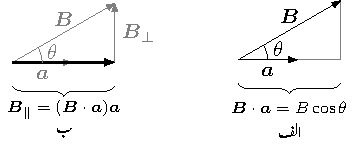
\includegraphics{figVectorComponentAlongUnitVector}
\caption{کسی بھی سمت میں سمتیہ کے جزو کا حصول۔}
\label{شکل_سمتیہ_کسی_سمت_میں_جزو}
\end{figure}
شکل \حوالہ{شکل_سمتیہ_کسی_سمت_میں_جزو}-الف میں سمتیہ \عددیء{\kvec{B}} اور اکائی سمتیہ \عددیء{\kvec{a}}  دکھائے گئے ہیں۔ان کا غیر سمتی ضرب
\begin{align*}
\kvec{B} \cdot \kvec{a} = \abs{\kvec{B}} \abs{\kvec{a}} \cos \theta=B \cos \theta
\end{align*}
کے برابر ہے۔شکل سے واضح ہے کہ یہی \عددیء{\kvec{a}} کی سمت میں \عددیء{\kvec{B}} کے جزو کا طول \عددیء{B_{\parallel}}\حاشیہد{\عددیء{B_{\parallel}} لکھتے ہوئے زیرنوشت میں دو متوازی لکیریں  یہ بتلاتی ہیں کہ \عددیء{\kvec{B}} کا یہ وہ حصہ ہے جو \عددیء{\kvec{a}} کے متوازی ہے۔اسی طرح عمودی مقدار کو عموماً \عددیء{\perp} کی علامت سے ظاہر کیا جاتا ہے۔} ہے۔یوں کسی بھی سمت میں \عددیء{\kvec{B}} کے جزو کا طول حاصل کرنے کی خاطر \عددیء{\kvec{B}} اور اس سمت کی اکائی سمتیہ کا غیر سمتی ضرب حاصل کریں۔یوں حاصل طول کا اکائی سمتیہ کے ساتھ ضرب یعنی \عددیء{(\kvec{B} \cdot \kvec{a}) \kvec{a}} سے اکائی سمتیہ کی سمت میں \عددیء{\kvec{B}} کا سمتی جزو  حاصل ہوتا ہے۔ شکل \حوالہ{شکل_سمتیہ_کسی_سمت_میں_جزو}-ب میں \عددیء{\kvec{a}} کی سمت میں \عددیء{\kvec{B}} کا سمتی جزو \عددیء{\kvec{B}_\parallel} دکھایا گیا ہے۔شکل سے واضح ہے کہ \عددیء{\kvec{B}} سے \عددیء{B_{\parallel} \kvec{a}} منفی کرنے سے  \عددیء{B_\perp} حاصل ہوتا ہے جو \عددیء{\kvec{B}} کا وہ جزو ہے جو \عددیء{\kvec{a}} کے عمودی ہے۔

غیر سمتی ضرب کا حاصل جواب دو صورتوں میں صفر کے برابر ہوتا ہے۔پہلی صورت وہ ہے جب دونوں سمتیوں میں سے کم از کم ایک سمتیہ کا طول صفر کے برابر ہو۔دوسری صورت وہ ہے جب دونوں سمتیات آپس میں عمودی ہوں۔عمودی ہونے کی صورت میں ان کے مابین نوے درجے کا زاویہ ہو گا اور \عددیء{\cos 90=0} کے برابر ہوتا ہے۔یوں دو سمتیوں کے نقطہ ضرب صفر کے برابر ہونے  سے اخذ کیا جاتا ہے کہ یہ آپس میں عمودی ہیں۔ 
%=================

\ابتدا{مثال}
شکل \حوالہ{شکل_سمتیہ_مثال_عمودی_سمتیات_کا_نقطہ_ضرب_صفر} میں تین نقطے \عددیء{M(1,5,6)}، \عددیء{N(4,3,1)} اور \عددیء{P(1,1,4)} دئے گئے ہیں۔\عددیء{M}  اور \عددیء{N} سے گزرتی سیدھی لکیر سے \عددیء{P} کا عمودی فاصلہ حاصل کریں۔ 
\begin{figure}
\centering
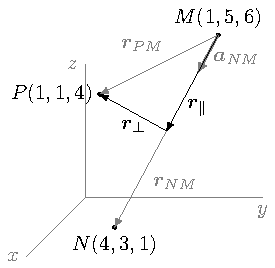
\includegraphics{figVectorExampleOrthognalVectorsHaveZeroDotProdcut}
\caption{متوازی اور عمودی اجزاء۔}
\label{شکل_سمتیہ_مثال_عمودی_سمتیات_کا_نقطہ_ضرب_صفر}
\end{figure}

حل:\عددیء{M} سے \عددیء{N} تک سمتیہ \عددیء{\kvec{r}_{NM}=3\ax-2\ay-5\az} ہے جس کا طول \عددیء{\abs{\kvec{r}_{NM}}=\sqrt{38}} ہے۔یوں اس سمت میں اکائی سمتیہ \عددیء{\kvec{a}_{NM}=\tfrac{3\ax-2\ay-5\az}{\sqrt{38}}} ہو گا۔ اسی طرح \عددیء{M} سے \عددیء{P} تک سمتیہ \عددیء{\kvec{r}_{PM}=-4\ay-2\az} ہے۔\عددیء{\kvec{a}_{NM}} کی سمت میں \عددیء{\kvec{r}_{PM}} کا طول
\begin{align*}
r_{\parallel}=\kvec{r}_{PM} \cdot \kvec{a}_{NM}&=(-4\ay-2\az) \cdot \left(\frac{3\ax-2\ay-5\az}{\sqrt{38}}\right) \\
&=\frac{0+8+10}{\sqrt{38}}=\frac{18}{\sqrt{38}}
\end{align*}
ہے یوں \عددیء{\kvec{a}_{NM}} سمت میں \عددیء{\kvec{r}_{PM}} کا سمتی جزو
\begin{align*}
\kvec{r}_{\parallel}=r_{\parallel} \kvec{a}_{NM}=\frac{18}{\sqrt{38}}\left(\frac{3\ax-2\ay-5\az}{\sqrt{38}}\right)=\frac{18}{38} (3\ax-2\ay-5\az)
\end{align*}
ہے۔\عددیء{\kvec{r}_{PM}} سے \عددیء{\kvec{r}_{\parallel}} منفی کرنے سے لکیر سے \عددیء{P} تک عمودی سمتیہ \عددیء{\kvec{r}_\perp} حاصل ہوتا ہے
\begin{align*}
\kvec{r}_{\perp}=\kvec{r}_{PM}-\kvec{r}_{\parallel}&=(-4\ay-2\az)-\frac{18}{38} (3\ax-2\ay-5\az)\\
&=\frac{-27\ax-58\ay+7\az}{19}
\end{align*}
جس کا طول \عددیء{\tfrac{\sqrt{27^2+58^2+7^2}}{19}=3.3873} ہے۔یوں \عددیء{P} کا لکیر سے عمودی فاصلہ \عددیء{3.3873} ہے۔

\عددیء{\kvec{r}_{\parallel}} اور \عددیء{\kvec{r}_\perp} آپس میں عمودی ہیں لہٰذا ان  کا نقطہ ضرب
\begin{align*}
\kvec{r}_\parallel \cdot \kvec{r}_\perp&=\frac{18}{38} (3\ax-2\ay-5\az) \cdot \left(\frac{-27\ax-58\ay+7\az}{19}\right)=\frac{18}{722}(-81+116-35)=0
\end{align*}
صفر کے برابر ہے۔
\انتہا{مثال}
%===================

شکل \حوالہ{شکل_سمتیہ_مثال_عمودی_سمتیات_کا_نقطہ_ضرب_صفر} میں اگر \عددیء{M} پر \عددیء{\kvec{r}_{NM}} کی دُم رکھی جائے تب  \عددیء{\kvec{r}_{NM}} کی نوک \عددیء{N} کا مقام تعین کرتا ہے۔عموماً کسی بھی نقطے کا مقام محدد کے مرکز \عددیء{(0,0,0)} کی نسبت سے طے کیا جاتا ہے۔ایسا سمتیہ جس کی دُم مرکز پر رکھتے ہوئے اس کی نوک نقطے کا مقام طے کرے  \اصطلاح{مقام تعین کنندہ} سمتیہ\فرہنگ{مقام تعین کنندہ!سمتیہ}\حاشیہب{displacement vector}\فرہنگ{displacement vector} کہلاتا ہے۔اگر تعین کنندہ سمتیہ کو مرکز سے ہٹایا جائے تب ظاہر ہے اس کی نوک اصل مقام طے کرنے سے قاصر ہو گی۔
%=======================================
\ابتدا{مثال}
شکل \حوالہ{شکل_سمتیہ_مثال_عمودی_سمتیات_کا_نقطہ_ضرب_صفر} میں \عددیء{M} سے شروع ہوتے اور  \عددیء{N} جانب بڑھتی سیدھی لکیر پر کسی بھی نقطے کا مقام تعین کرتے تعین کنندہ سمتیہ حاصل کریں۔

حل:مرکز \عددیء{(0,0,0)} سے  نقطہ \عددیء{M} تک کا سمتیہ \عددیء{\kvec{r}_M=1\ax+5\ay+6\az} ہے جبکہ \عددیء{M} سے \عددیء{N} جانب اکائی سمتیہ \عددیء{\kvec{a}_{NM}} گزشتہ مثال میں حاصل کیا گیا۔اکائی سمتیہ \عددیء{\kvec{a}_{NM}} کی سمت میں  \عددیء{M} سے \عددیء{s} فاصلے پر نقطہ \عددیء{Q} تک کا سمتیہ \عددیء{s\kvec{a}_{NM}} ہے۔یوں مرکز سے  \عددیء{Q} تک سمتیہ \عددیء{\kvec{r}_Q=\kvec{r}_M+s\kvec{a}_{NM}} ہو گا۔
\begin{align*}
\kvec{r}_Q=(1\ax+5\ay+6\az) +s \left(\frac{3\ax-2\ay-5\az}{\sqrt{38}}\right)
\end{align*}   
اس مساوات میں \عددیء{s} متغیرہ ہے جسے تبدیل کرتے ہوئے سیدھی لکیر پر کسی بھی نقطہ \عددیء{Q} تک پہنچا جا سکتا ہے۔
\انتہا{مثال}
%==========================
\ابتدا{مثال}
\عددیء{z=z_0} پر \عددیء{1\az} کے عمودی سیدھی سطح کی مساوات حاصل کریں جہاں \عددیء{z_0} مستقل ہے۔ 

حل:نقطہ \عددیء{N_1(0,0,z_0)} سے کسی بھی نقطہ \عددیء{N_2(x,y,z)} تک کا سمتیہ \عددیء{\kvec{r}_{21}=x\ax+y\ay+(z-z_0)\az} ہے۔سطح پر کسی بھی سمتیہ اور سطح کے عمودی سمتیہ آپس میں نوے درجے زاویہ پر پائے جاتے ہیں لہٰذا ان کا غیر سمتی ضرب صفر کے برابر ہو گا۔یوں اگر \عددیء{N_2} اسی عمودی سطح پر پایا جائے تب
\begin{align*}
1\az \cdot [x\ax+y\ay+(z-z_0)\az]=z-z_0=0
\end{align*}
ہو گا جس سے اس سطح کی مساوات \عددیء{z=z_0} حاصل ہوتی ہے۔

اس قیمت کو \عددیء{\kvec{r}_{21}} میں پُر کرتے ہوئے \عددیء{\kvec{r}_{21}=x\ax+y\ay} حاصل ہوتا ہے جہاں \عددیء{x} اور \عددیء{y} آزاد متغیرات ہیں۔چونکہ مرکز سے \عددیء{N_1} کا تعین کنندہ سمتیہ \عددیء{\kvec{r}_{10}=z_0\az} ہے لہٰذا \عددیء{z=z_0} سطح پر کسی بھی نقطہ \عددیء{N_2} کا تعین کنندہ سمتیہ یعنی سطح کی سمتی مساوات  \عددیء{\kvec{r}_{20}=x\ax+y\ay+z_0\az} ہو گی۔
\انتہا{مثال}
%==========
\ابتدا{مشق}
مرکز سے \عددیء{(2,1,3)} تک کی سمتیہ ایک سیدھی سطح کی عمودی سمتیہ ہے۔اس سطح کی  مساوات حاصل کریں۔

جواب:\عددیء{2x+y+3z=14}
\انتہا{مشق}
%============
\حصہ{سمتی ضرب یا صلیبی ضرب}

دو سمتیات \عددیء{\kvec{A}} اور \عددیء{\kvec{B}} کے \اصطلاح{سمتی ضرب}\فرہنگ{سمتی ضرب}\فرہنگ{صلیبی ضرب}\حاشیہب{vector product}\فرہنگ{vector product} کا حاصل جواب سمتیہ ہوتا ہے جس کا طول \عددیء{\kvec{A}} کی مقدار ضربِ  \عددیء{\kvec{B}} کی مقدار ضربِ سمتیوں کے مابین چھوٹے زاویے کے سائن کے برابر ہے۔حاصل سمتیہ \عددیء{\kvec{A}} اور \عددیء{\kvec{B}} سمتیات کی عمودی سمت  میں ہوتا ہے جسے اکائی عمودی سمتیہ \عددیء{\kvec{a}_N} سے ظاہر کیا جائیگا۔
\begin{align}\label{مساوات_سمتیہ_سمتی_ضرب}
\kvec{A} \times \kvec{B}=\abs{\kvec{A}} \abs{\kvec{B}} \sin \theta_{AB} \kvec{a}_N
\end{align}
جس سیدھی سطح پر \عددیء{\kvec{A}} اور \عددیء{\kvec{B}} دونوں پائے جائیں، \عددیء{\kvec{a}_N} اس سطح کے دو عمودی سمتیات میں سے ایک ہے۔\عددیء{\kvec{a}_N} کو \اصطلاح{دائیں ہاتھ کے قانون}\فرہنگ{دائیں ہاتھ!قانون}\حاشیہب{right hand rule}\فرہنگ{right hand rule} سے یوں حاصل کیا جا سکتا ہے۔

\ابتدا{قانون}\شناخت{قانون_سمتیہ_دائیں_ہاتھ_قانون}
دائیں ہاتھ کی ہتھیلی  سیدھی اور انگوٹھے کو بقایا چار انگلیوں کے عمود میں رکھتے ہوئے پہلی انگلی کو \عددیء{\kvec{A}} اور  دوسری انگلی کو \عددیء{\kvec{B}} کی سمت میں رکھیں۔اس صورت میں انگوٹھا \عددیء{\kvec{a}_N} کی سمت میں ہو گا۔  
\انتہا{قانون}

اگر دونوں سمتیات کی دُم ایک ہی جگہ پر نہ ہو تب ان کے مابین زاویہ دریافت کرنے کی  خاطر سمتیوں کی سمت تبدیل کئے بغیر انہیں ایک نقطے پر منتقل کیا جا سکتا ہے۔سمتی ضرب کو سمتیوں کے درمیان صلیبی نشان \عددیء{\times} سے ظاہر کیا جاتا ہے۔اسی وجہ سے اسے \اصطلاح{صلیبی ضرب}\حاشیہب{cross product}\فرہنگ{cross product} بھی کہا جاتا ہے اور \عددیء{\kvec{A} \times \kvec{B}} کو "\عددیء{\kvec{A}} صلیب \عددیء{\kvec{B}}" پڑھا جاتا ہے۔سمتی ضرب میں سمتیوں کی ترتیب نہایت اہم ہے اور انہیں الٹانے سے حاصل جواب کی سمت الٹی ہو جاتی ہے۔
\begin{align}\label{مساوات_سمتیہ_صلیبی_ضرب_ترتیب_الٹاتے_منفی_سمت}
\kvec{A} \times \kvec{B}=- \kvec{B} \times \kvec{A}
\end{align}

اکائی سمتیات \عددیء{\ax} اور \عددیء{\ay} کے مابین نوے درجے کا زاویہ ہے  اور \عددیء{\sin 90\degree=1} کے برابر ہے جبکہ دائیں ہاتھ کے قانون سے ان کے صلیبی ضرب کی سمت \عددیء{\az} حاصل ہوتی ہے۔یوں \عددیء{\ax \times \ay=\az} کے برابر ہے۔اسی طرح \عددیء{\ay \times \az=\ax} اور \عددیء{\az \times \ax=\ay} کے برابر حاصل ہوتے ہیں۔مساوات \حوالہ{مساوات_سمتیہ_صلیبی_ضرب_ترتیب_الٹاتے_منفی_سمت} کے تحت یوں \عددیء{\ay \times \ax=-\az}، \عددیء{\az \times \ay=-\ax} اور \عددیء{\ax \times \az=-\ay} لکھے جا سکتے ہیں۔دو متوازی سمتیوں کے درمیان صفر درجے کا زاویہ ہوتا ہے اور \عددیء{\sin 0 =0} کے برابر ہے لہٰذا \عددیء{\ax \times \ax=0} کے برابر ہے۔اسی طرح \عددیء{\ay \times \ay=0} اور \عددیء{\az \times \az=0} کے برابر ہیں۔ان تمام جوابات کو ایک جگہ لکھتے ہیں۔
\begin{gather}
\begin{aligned}\label{مساوات_سمتیہ_کارتیسی_اکائی_سمتیات_صلیبی_ضرب}
\ax \times \ay &=\az & \ay \times \az&=\ax & \az \times \ax&=\ay\\
\ax \times \ax&=0 & \ay \times \ay&=0 & \az \times \az&=0
\end{aligned}
\end{gather}
%=================

یہی جوابات شکل \حوالہ{شکل_سمتیہ_صلیبی_ضرب_مثبت_دائرہ} کی مدد سے حاصل کئے جا سکتے ہیں۔اس شکل میں گھڑی کی الٹ سمت مثبت سمت ہے۔یوں اگر \عددیء{\ax \times \ay} حاصل کرنا ہو تو شکل میں \عددیء{\ax} سے شروع ہو کر \عددیء{\ay} کی جانب کم راستے پر چلتے ہوئے  \عددیء{\az} حاصل ہوتا ہے۔ساتھ ہی ساتھ چونکہ \عددیء{\ax} سے \عددیء{\ay} جانے کی خاطر  مثبت راستہ اختیار کیا گیا لہٰذا جواب مثبت یعنی \عددیء{+\az} ہو گا۔اس کے برعکس \عددیء{\az \times \ay} حاصل کرنے کی خاطر \عددیء{\az} سے \عددیء{\ay} جانب کم راستے پر چلتے ہوئے \عددیء{\ax} حاصل ہوتا ہے البتہ یہ راستہ گھڑی کے الٹ سمت یعنی منفی سمت میں ہے لہٰذا جواب \عددیء{-\ax} ہو گا۔ 
\begin{figure}
\centering
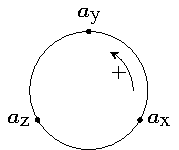
\includegraphics{figVectorCartesianRightHandCircle}
\caption{صلیبی ضرب کا حصول۔}
\label{شکل_سمتیہ_صلیبی_ضرب_مثبت_دائرہ}
\end{figure}

مساوات \حوالہ{مساوات_سمتیہ_کارتیسی_اکائی_سمتیات_صلیبی_ضرب} کی  مدد سے \عددیء{\kvec{A}=A_x\ax+A_y\ay+A_z\az} اور \عددیء{\kvec{B}=B_x\ax+B_y\ay+B_z\az} کی صلیبی ضرب
\begin{align*}
\kvec{A} \times \kvec{B}&=(A_x\ax+A_y\ay+A_z\az) \times (B_x\ax+B_y\ay+B_z\az)\\
&=A_x B_x \ax \times \ax+A_x B_y \ax \times \ay+A_x B_z \ax \times \az\\
& \quad \quad +A_y B_x \ay \times \ax+A_y B_y \ay \times \ay+A_y B_z \ay \times \az \\
&\quad \quad +A_z B_x \az \times \ax+A_z B_y \az \times \ay+A_z B_z \az \times \az
\end{align*}
کو
\begin{align}
\kvec{A} \times \kvec{B}=(A_y B_z-A_z B_y)\ax+(A_z B_x-A_x B_z)\ay+(A_x B_y-A_y B_x)\az
\end{align}
لکھا جا سکتا ہے۔اس جواب کو قالب کے حتمی قیمت کی شکل میں یوں لکھا جا سکتا ہے۔
\begin{align}\label{مساوات_سمتیات_سمتی_ضرب_قالب_شکل}
\kvec{A} \times \kvec{B}=\begin{vmatrix}
\ax & \ay & \az\\
A_x & A_y & A_z\\
B_x & B_y & B_z
\end{vmatrix}
\end{align}
مندرجہ بالا قالب کو کتاب کے آخر میں صفحہ \حوالہصفحہ{ضمیمہ_خطی_الجبرا} پر ضمیمے میں آپ کے آسانی کے لئے دوبارہ پیش کیا گیا ہے۔اس ضمیمے کو ایک مرتبہ دیکھ لیں۔
یوں اگر \عددیء{\kvec{A}=2\ax-3\ay+1\az} اور \عددیء{\kvec{B}=6\ax+5\ay-4\az} ہوں تب
\begin{align*}
\kvec{A} \times \kvec{B}&=\begin{vmatrix*}[r]
\ax & \ay & \az\\
2 & -3 & 1\\
6 & 5 & -4
\end{vmatrix*}\\
&=[(-3)(-4)-(1)(5)]\ax-[(2)(-4)-(1)(6)]\ay+[(2)(5)-(-3)(6)]\az\\
&=7\ax+14\ay+28\az
\end{align*}
ہو گا۔
%===========
\ابتدا{مثال}
\عددیء{N_1(2,3,1)}، \عددیء{N_2(1,6,5)} اور \عددیء{N_3(-2,-3,2)} سیدھی سطح پر پائے جاتے ہیں۔اس سطح کی مساوات حاصل کریں۔

حل:
\begin{align*}
\kvec{r}_{21}&=(1-2)\ax+(6-3)\ay+(5-1)\az=-1\ax+3\ay+4\az\\
\kvec{r}_{31}&=(-2-2)\ax+(-3-3)\ay+(2-1)\az=-4\ax-6\ay+1\az
\end{align*}
کے سمتی ضرب سے ان کا عمودی سمتیہ حاصل ہو گا۔
\begin{align*}
\kvec{r}_N&=(-1\ax+3\ay+4\az) \times (-4\ax-6\ay+1\az)\\
&=6\az+1\ay+12\az+3\ax-16\ay+24\ax\\
&=27\ax-15\ay+18\az
\end{align*}
سطح پر دئے گئے تین نقطوں سے سطح پر کسی بھی نقطہ \عددیء{N_4(x,y,z)} تک کا سمتیہ اس عمودی سمتیہ کے نوے درجے زاویہ پر ہو گا اور یوں ان کا غیر سمتی ضرب صفر کے برابر ہو گا۔\عددیء{N_1} سے \عددیء{N_4} تک سمتیہ \عددیء{\kvec{r}_{41}=(x-2)\ax+(y-3)\ay+(z-1)\az} کے استعمال سے
\begin{align*}
\kvec{r}_{41} \cdot \kvec{r}_{N}=[(x-2)\ax+(y-3)\ay+(z-1)\az] \cdot (27\ax-15\ay+18\az)=0
\end{align*}
لکھ کر
\begin{align*}
27(x-2)-15(y-3)+18(z-1)=0
\end{align*}
سے
\begin{align*}
27x-15y+18z=27
\end{align*}
سیدھی سطح کی مساوات حاصل ہوتی ہے۔ایسی مساوات میں \عددیء{x}، \عددیء{y} اور \عددیء{z} کے مخفف عمودی سمتیہ میں \عددیء{\ax}، \عددیء{\ay} اور \عددیء{\az} کے مخفف \عددیء{27}، \عددیء{-15} اور \عددیء{18} ہوتے ہیں۔

سطح کی مساوات سے \عددیء{z=\tfrac{9-9x+5y}{6}} لکھا جا سکتا ہے۔سطح پر \عددیء{N_4} کی تعین کنندہ مساوات \عددیء{\kvec{r}=x\ax+y\ay+z\az} میں \عددیء{z} کی قیمت پُر کرتے ہوئے  سطح کی سمتی مساوات 
\begin{align*}
\kvec{r}=x\ax+y\ay+\left(\frac{9-9x+5y}{6}\right)\az
\end{align*}
لکھی جا سکتی ہے جہاں \عددیء{x} اور \عددیء{y} آزاد متغیرات ہیں جبکہ \عددیء{z} کو بطور تابع متغیرہ لکھا گیا ہے۔
\انتہا{مثال}
%=========

\ابتدا{مشق}
\عددیء{\kvec{A}=1\ax+3\ay-2\az} اور \عددیء{\kvec{B}=5\ax-2\ay-3\az} کی صورت میں \عددیء{\kvec{A} \times \kvec{B}}، \عددیء{\kvec{B}\times \kvec{A}}، \عددیء{\kvec{A} \times \kvec{A}}، \عددیء{\kvec{a}_B \times \kvec{A}} اور \عددیء{\az \times (\ay \times \kvec{B})} حاصل کریں۔ 
\انتہا{مشق}
%========================

خلاء میں کسی بھی نقطے کا مقام کارتیسی محدد کے علاوہ دیگر طرز کے محدد سے بھی تعین کیا جا سکتا ہے۔ماہرین طبیعیات  تقریباً ایک درجن اقسام کے محددی نظام استعمال کرتے ہیں۔ہم اس کتاب میں کارتیسی نظام کے علاوہ دو مزید اقسام کے محددی نظام استعمال کریں گے۔آئیں انہیں پر غور کریں۔ 

\حصہ{گول نلکی محدد}
کارتیسی نظام میں کسی بھی نقطے کا مقام مرکز سے \عددیء{x}، \عددیء{y} اور \عددیء{z} سمتوں میں فاصلوں سے طے کیا جاتا ہے۔آئیں اب ایسا نظام دیکھیں جس میں ایک عدد زاویہ اور دو عدد فاصلے استعمال کرتے ہوئے کسی بھی نقطے کا مقام طے ہو۔
 \begin{figure}
\centering
\begin{subfigure}{0.4\textwidth}
\centering
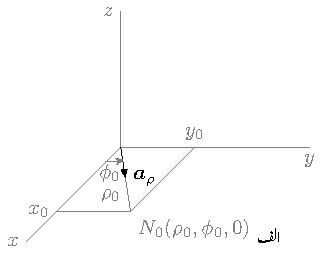
\includegraphics{figVector2and3Dcylindrical}
\end{subfigure}%
%
\begin{subfigure}{0.4\textwidth}
\centering
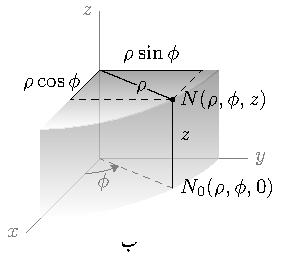
\includegraphics{figVectorCylindricalToCartesian}
\end{subfigure}%
\caption{نلکی محدد}
\label{شکل_سمتیہ_نلکی_محدد}
\end{figure}

شکل \حوالہ{شکل_سمتیہ_نلکی_محدد}-الف میں \عددیء{z=0} سطح پر نقطہ \عددیء{N_0} دکھایا گیا ہے جسے کارتیسی محدد میں \عددیء{N_0(x_0,y_0,0)} لکھا جائے گا۔اگر مرکز سے \عددیء{N_0} تک سیدھی لکیر کی لمبائی \عددیء{\rho_0} اور \عددیء{x} محدد سے اس لکیر کا زاویہ \عددیء{\phi_0} ہو تب اسی نقطے
 کو \اصطلاح{گول نلکی محدد}\فرہنگ{نلکی!محدد}\حاشیہب{cylindrical coordinate system}\فرہنگ{cylindrical!coordinates} کے نظام میں \عددیء{N_0(\rho_0,\phi_0,0)} لکھا جاتا ہے۔اس کتاب میں گول نلکی محدد کا نام چھوٹا کر کے اسے \اصطلاح{نلکی محدد} پکارا جائے گا۔ اگر \عددیء{z=0} سطح پر مرکز سے نقطے کی جانب اکائی سمتیہ \عددیء{\arho} ہو تب مرکز سے نقطے تک سمتیہ کو
\begin{align}
\kvec{\rho}=\rho_0 \arho \quad \quad (\phi=\phi_0, \quad   z=0 )
\end{align}
   لکھا جا سکتا ہے۔نلکی  اور کارتیسی نظام میں  \عددیء{z} محدد یکساں ہیں۔

شکل \حوالہ{شکل_سمتیہ_نلکی_محدد} سے کارتیسی اور نلکی محدد کے تعلق اخذ کئے جا سکتے ہیں۔یوں نلکی محدد کے متغیرات \عددیء{(\rho,\phi,z)} سے کارتیسی متغیرات \عددیء{(x,y,z)} یوں حاصل ہوتے ہیں۔
\begin{gather}
\begin{aligned}
x&=\rho \cos \phi\\
y&=\rho \sin \phi\\
z&=z
\end{aligned}
\end{gather}
اسی طرح \عددیء{(x,y,z)} سے  \عددیء{(\rho,\phi,z)} یوں حاصل کئے جاتے ہیں۔
\begin{gather}
\begin{aligned}
\rho&=\sqrt{x^2+y^2} \quad \quad (\rho \ge 0)\\
\phi&=\tan^{-1} \frac{y}{x}\\
z&=z
\end{aligned}
\end{gather}
%
درج بالا دونوں تعلقات کو کتاب کے آخر میں صفحہ \حوالہصفحہ{ضمیمہ_محددی_تعلق} پر ضمیمے میں دوبارہ پیش کیا گیا ہے۔
\begin{figure}
\centering
\begin{subfigure}{0.4\textwidth}
\centering
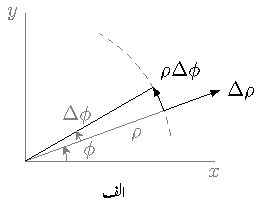
\includegraphics{figVectorCylindricalRadiusAngle}
\end{subfigure}%
%
\begin{subfigure}{0.4\textwidth}
\centering
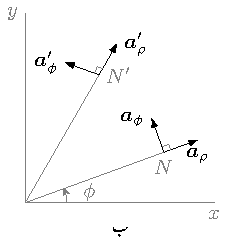
\includegraphics{figVectorCylindricalUnitVectors}
\end{subfigure}%
\caption{نلکی محدد میں متغیرات کے تبدیلی سے فاصلے کا حصول اور اکائی سمتیات۔}
\label{شکل_سمتیہ_نلکی_تبدیلی_متغیرات}
\end{figure}
مندرجہ بالا مساوات میں رداس کی صرف مثبت قیمت لی گئی۔ہم  رداس کی قیمت مثبت ہی لیتے ہیں۔

شکل \حوالہ{شکل_سمتیہ_نلکی_تبدیلی_متغیرات}-الف میں \عددیء{\phi} زاویہ پر \عددیء{\rho} رداس کا ہلکی سیاہی میں دکھایا سمتیہ نقطہ \عددیء{N} ہے۔
اس شکل میں \عددیء{\phi} اور \عددیء{z} تبدیل کئے بغیر \عددیء{\rho} کو \عددیء{\Delta \rho} بڑھتا دکھایا گیا ہے۔اس صورت میں سمتیہ کی نوک \عددیء{\Delta \rho} فاصلہ طے کرتی ہے۔نقطہ \عددیء{N} سے \عددیء{\Delta \rho} کی سمت میں اکائی سمتیہ جسے \عددیء{\arho} لکھا جاتا ہے، نلکی محدد کی  بنیادی اکائی سمتیہ ہے۔اس سمتیہ کو شکل \حوالہ{شکل_سمتیہ_نلکی_تبدیلی_متغیرات}-ب میں دکھایا گیا ہے۔

شکل \حوالہ{شکل_سمتیہ_نلکی_تبدیلی_متغیرات}-الف میں   \عددیء{\rho} اور \عددیء{z} تبدیل کئے بغیر \عددیء{\phi} کو \عددیء{\Delta \phi} بڑھا کر اسی سمتیہ کو گاڑھی سیاہی میں دوبارہ دکھایا گیا ہے۔آپ دیکھ سکتے ہیں کہ  سمتیہ کی نوک نے \عددیء{\rho} رداس کے گول دائرے پر حرکت کرتے ہوئے  \عددیء{\rho \Delta \phi} فاصلہ طے کیا۔یوں اگر زاویہ کو \عددیء{0} تا \عددیء{2\pi} ریڈیئن تبدیل کیا جائے  تو سمتیہ کی نوک گول دائرے پر ایک مکمل چکر کاٹے گی۔جیسے جیسے \عددیء{\Delta \phi} کو کم سے کم کیا جائے ویسے ویسے  \عددیء{\rho \Delta \phi}  گول دائرے کے مماس کی صورت اختیار کرے گی حتٰی کہ \عددیء{\dif \phi} کی صورت میں \عددیء{\rho \dif \phi} گول دائرے کا مماس ہو گا۔نقطہ \عددیء{N} پر بڑھتے \عددیء{\phi} جانب مماس کی سمت میں اکائی سمتیہ کو \عددیء{\aphi} لکھا جاتا ہے۔ اس سمتیہ کو شکل \حوالہ{شکل_سمتیہ_نلکی_تبدیلی_متغیرات}-ب میں دکھایا گیا ہے۔

اسی طرح اگر نقطہ \عددیء{N} پر صرف \عددیء{z} کو \عددیء{\Delta z} تبدیل کیا جائے تب سمتیہ کی نوک \عددیء{\Delta z} فاصلہ طے کرے گی۔ \عددیء{\Delta z} کی سمت میں اکائی سمتیہ جسے \عددیء{\az} لکھا جاتا ہے، نلکی محدد کی تیسری اور آخری بنیادی اکائی سمتیہ ہے۔نلکی محدد کے تین اکائی سمتیات \عددیء{\arho}، \عددیء{\aphi} اور \عددیء{\az} مل کر دائیں ہاتھ کا عمودی  نظام دیتے ہیں۔نقطہ \عددیء{(\rho_1,\phi_1,z_1)} پر نلکی محدد کے اکائی سمتیات کو شکل \حوالہ{شکل_سمتیہ_نلکی_اکائی_سمتیات_عمومی} میں دکھایا گیا ہے۔\عددیء{\arho} گول سطح \عددیء{\rho=\rho_1} کے عمودی ہے۔یہ \عددیء{\phi=\phi_1} اور \عددیء{z=z_1} سطحوں پر پایا جاتا ہے۔اسی طرح \عددیء{\aphi} سیدھی سطح  \عددیء{\phi=\phi_1} کے عمودی ہے۔ یہ \عددیء{z=z_1} سطح پر پایا جاتا ہے اور \عددیء{\rho=\rho_1} نلکی سطح کا مماس ہے۔\عددیء{\az} اکائی سمتیہ \عددیء{z=z_1} سطح کے عمودی ہے۔یہ \عددیء{\rho=\rho_1} اور \عددیء{\phi=\phi_1} سطحوں پر پایا جاتا ہے۔ 
\begin{figure}
\centering
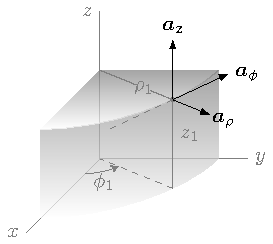
\includegraphics{figVectorCylindricalUnitVectorDirectionsInThreeD}
\caption{نلکی محدد کے اکائی سمتیات۔}
\label{شکل_سمتیہ_نلکی_اکائی_سمتیات_عمومی}
\end{figure}

دائیں ہاتھ کے عمودی نظام میں سمتی ضرب کا حاصل جواب صفحہ \حوالہصفحہ{قانون_سمتیہ_دائیں_ہاتھ_قانون} پر دئے گئے دائیں ہاتھ کے قانون کی مدد سے حاصل کیا جاتا ہے ۔ یوں
\begin{align}\label{مساوات_سمتیات_نلکی_اکائی_سمتیات_کا_سمتی_ضرب}
\arho \times \aphi=\az, \quad \aphi \times \az=\arho, \quad \az \times \arho=\aphi
\end{align}
لکھا جا سکتا ہے۔یہی جوابات شکل \حوالہ{شکل_سمتیہ_نلکی_صلیبی_ضرب_مثبت_دائرہ} سے بھی اخذ کئے جا سکتے ہیں۔
\begin{figure}
\centering
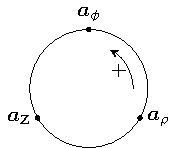
\includegraphics{figVectorCylindricalRightHandCircle}
\caption{صلیبی ضرب کی حاصل اکائی سمتیہ۔}
\label{شکل_سمتیہ_نلکی_صلیبی_ضرب_مثبت_دائرہ}
\end{figure}

کسی سمتیہ کا خود سمتی ضرب صفر کے برابر ہوتا ہے لہٰذا
\begin{align}\label{مساوات_سمتیات_نلکی_اکائی_سمتیات_کا_سمتی_ضرب_ب}
\arho \times \arho=0, \quad \aphi \times \aphi =0, \quad \az \times \az=0
\end{align}
لکھا جا سکتا ہے جبکہ کسی بھی اکائی سمتیہ کا خود غیر سمتی ضرب ایک کے برابر ہوتا ہے لہٰذا 
\begin{align}
\arho \cdot \arho=1, \quad \aphi \cdot \aphi =1, \quad \az \cdot \az =1
\end{align}
لکھا جا سکتا ہے۔اسی طرح کسی بھی دو عمودی سمتیات  کا غیر سمتی ضرب صفر کے برابر ہوتا ہے یعنی
\begin{align}
\arho \cdot \aphi=0, \quad \aphi \cdot \az =0, \quad \az \cdot \arho =0
\end{align}

غیر سمتی ضرب کو  \اصطلاح{کرونیکر ڈیلٹا} کی مدد سے یوں لکھا جا سکتا ہے۔
\begin{align}
\kvec{a}_i \cdot \kvec{a}_j=\delta_{ij}
\end{align}
جہاں
\begin{align}
\delta_{ij}=
\begin{cases}
0 \quad  \quad  i\ne j \; \textup{ اگر}\\
1 \quad \quad i=j \; \textup{ اگر}
\end{cases}
\end{align}
کے برابر ہے۔

آپ دیکھتے ہیں کہ کسی بھی نقطہ \عددیء{N(\rho,\phi,z)} پر  اکائی سمتیات حاصل کرنے کی خاطر محدد کے متغیرات \عددیء{\rho}، \عددیء{\phi} اور \عددیء{z} کو  باری باری انتہائی کم بڑھایا جاتا ہے۔جس سمت میں نقطہ حرکت کرے، اسی سمت میں اکائی سمتیہ ہو گی۔شکل \حوالہ{شکل_سمتیہ_نلکی_تبدیلی_متغیرات}-ب میں دو مختلف نقاط \عددیء{N} اور \عددیء{N'} پر نلکی محدد کے عمودی اکائی سمتیات دکھائے گئے ہیں۔آپ دیکھ سکتے ہیں کہ نلکی محدد کے عمودی اکائی سمتیات کی سمت کا دارومدار اس نقطے پر ہے جہاں انہیں حاصل کیا جائے۔آپ جانتے ہیں کہ کارتیسی نظام میں نقطے کا مقام تبدیل کرنے سے کارتیسی اکائی سمتیات تبدیل نہیں ہوتے۔یوں نلکی محدد کے اکائی سمتیات اٹل نہیں ہیں۔یہ ایک انتہائی اہم حقیقت ہے جو تکمل لیتے وقت پیچیدگیاں پیدا کرتا ہے۔تکمل لیتے وقت کارتیسی اکائی سمتیات اٹل ہونے کی بنا پر تکمل کے باہر لے جائے جا سکتے ہیں جبکہ نلکی محدد کے  \عددیء{\arho} اور \عددیء{\aphi} اکائی سمتیات کو تکمل کے باہر نہیں لے جایا جا سکتا۔یاد رہے کہ کسی بھی نقطہ \عددیء{N} پر حاصل کئے گئے \عددیء{\arho}، \عددیء{\aphi} اور \عددیء{\az} آپس میں عمودی ہوں گے جبکہ کسی اور نقطہ \عددیء{N'} پر حاصل کئے گئے \عددیء{\arho'}، \عددیء{\aphi'} اور \عددیء{\az} آپس میں عمودی ہوں گے۔

\جزوحصہ{نلکی اکائی سمتیات کا کارتیسی اکائی سمتیات کے ساتھ غیر سمتی ضرب}
شکل \حوالہ{شکل_سمتیہ_نلکی_کارتیسی_اکائی_غیر_سمتی_ضرب}-الف میں نقطہ \عددیء{N} پر اکائی سمتیات \عددیء{\arho}، \عددیء{\ax} اور \عددیء{\ay} دکھائے گئے ہیں۔\عددیء{\arho} اور  \عددیء{\ax} کے مابین زاویہ \عددیء{\phi} ہے جبکہ اکائی سمتیات کی لمبائی ایک ہوتی ہے لہٰذا
\begin{align}
\arho \cdot \ax=(1)(1)(\cos \phi)=\cos \phi
\end{align}
ہے۔\عددیء{\arho} اور  \عددیء{\ay} کے مابین زاویہ \عددیء{(90^\circ-\phi)} ہے  لہٰذا
\begin{align}
\arho \cdot \ay=(1)(1)[\cos (90^\circ-\phi)]=\sin \phi
\end{align}
کے برابر ہے۔اس مساوات میں \عددیء{\cos(\alpha-\beta)=\cos \alpha \cos \beta+\sin \alpha \sin \beta} کو استعمال کرتے ہوئے \عددیء{\cos(90^\circ-\phi)=\sin \phi} لکھا گیا ہے۔شکل \حوالہ{شکل_سمتیہ_نلکی_کارتیسی_اکائی_غیر_سمتی_ضرب}-ب میں نقطہ \عددیء{N} پر اکائی سمتیات \عددیء{\aphi}، \عددیء{\ax} اور \عددیء{\ay} دکھائے گئے ہیں۔\عددیء{\aphi} اور  \عددیء{\ax} کے مابین زاویہ \عددیء{(90^\circ+\phi)} ہے  لہٰذا
\begin{align}
\aphi \cdot \ax=(1)(1)[\cos (90^\circ+\phi)]=-\sin \phi
\end{align}
ہے۔\عددیء{\aphi} اور  \عددیء{\ay} کے مابین زاویہ \عددیء{\phi} ہے  لہٰذا
\begin{align}
\aphi \cdot \ay=(1)(1)(\cos \phi)=\cos \phi
\end{align}
کے برابر ہے۔\عددیء{\az} کا \عددیء{\ax} اور \عددیء{\ay} کے ساتھ غیر سمتی ضرب صفر کے برابر ہے۔اس کی وجہ ان کے مابین نوے درجے کا زاویہ ہے۔ان تمام غیر سمتی ضرب کو جدول \حوالہ{جدول_سمتیہ_نلکی_کارتیسی_اکائی_غیر-سمتی_ضرب} میں یکجا کیا گیا ہے۔
\begin{figure}
\centering
\begin{subfigure}{0.4\textwidth}
\centering
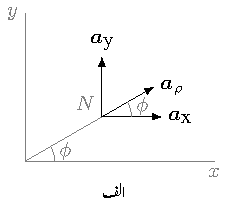
\includegraphics{figVectorCylindricalXandRhoDotProduct}
\end{subfigure}%
%
\begin{subfigure}{0.4\textwidth}
\centering
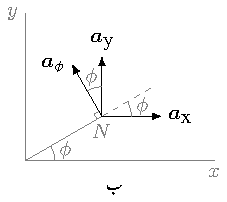
\includegraphics{figVectorCylindricalXandPhiDotProduct}
\end{subfigure}%
\caption{نلکی اکائی سمتیات کا کارتیسی اکائی سمتیات کے ساتھ غیر سمتی ضرب۔}
\label{شکل_سمتیہ_نلکی_کارتیسی_اکائی_غیر_سمتی_ضرب}
\end{figure}%
%
%
\begin{table}
\caption{نلکی اکائی سمتیات کا کارتیسی اکائی سمتیات کے ساتھ غیر سمتی ضرب۔}
\centering
\begin{tabular}{l | r r r}
 & $\ax$ & $\ay$ & $\az$ \\
\hline
$\arho$ & $\cos \phi$ & $\sin \phi $& $0$\\
$\aphi$ &$-\sin \phi$ &$ \cos \phi$ &$ 0$\\
$\az$ & $0$ &$ 0$ &$1$
\end{tabular}
\label{جدول_سمتیہ_نلکی_کارتیسی_اکائی_غیر-سمتی_ضرب}
\end{table}
%
\begin{figure}
\centering
\begin{subfigure}{0.4\textwidth}
\centering
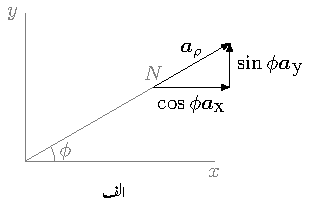
\includegraphics{figVectorCylindricalRhoToCartesianConversion}
\end{subfigure}%
%
\begin{subfigure}{0.4\textwidth}
\centering
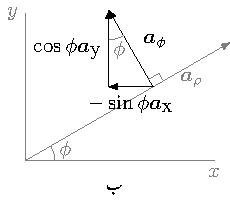
\includegraphics{figVectorCylindricalPhiToCartesianConversion}
\end{subfigure}%
\caption{\عددیء{\arho} اور \عددیء{\aphi} کا کارتیسی نظام میں تبادلہ۔}
\label{شکل_سمتیہ_کارتیسی_نظام_میں_نلکی_رداس_اکائی}
\end{figure}%

\جزوحصہ{نلکی اور کارتیسی اکائی سمتیات کا تعلق}
شکل \حوالہ{شکل_سمتیہ_کارتیسی_نظام_میں_نلکی_رداس_اکائی}-الف میں نقطہ \عددیء{N} پر اکائی سمتیہ \عددیء{\arho} دکھایا گیا ہے۔آپ دیکھ سکتے ہیں کہ کارتیسی محدد میں اسی اکائی سمتیہ کو دو عدد سمتیات کی مدد سے لکھا جا سکتا ہے۔\عددیء{\arho} کی لمبائی ایک کے برابر ہے۔یوں مسئلہ فیثاغورث کی مدد سے
\begin{gather}
\begin{aligned}\label{مساوات_سمتیہ_اکائی_رداس_کارتیسی_میں}
\arho&=\cos \phi \ax+\sin \phi \ay\\
&=\frac{x}{\sqrt{x^2+y^2}} \ax+\frac{y}{\sqrt{x^2+y^2}} \ay
\end{aligned}
\end{gather}
 لکھا جا سکتا ہے جہاں دوسرے قدم پر تمام نلکی محدد کے متغیرات کو کارتیسی متغیرات کی شکل میں لکھا گیا ہے۔شکل \حوالہ{شکل_سمتیہ_کارتیسی_نظام_میں_نلکی_رداس_اکائی}-ب میں نقطہ \عددیء{N} پر اکائی سمتیہ \عددیء{\aphi} دکھایا گیا ہے۔آپ دیکھ سکتے ہیں کہ کارتیسی محدد میں اسی اکائی سمتیہ کو دو عدد سمتیات کی مدد سے یوں  لکھا جا سکتا ہے
\begin{gather}
\begin{aligned}\label{مساوات_سمتیہ_اکائی_زاویہ_کارتیسی_میں}
\aphi&=-\sin \phi \ax+\cos \phi \ay\\
&=-\frac{y}{\sqrt{x^2+y^2}} \ax+\frac{x}{\sqrt{x^2+y^2}} \ay
\end{aligned}
\end{gather}
جہاں دوسرے قدم پر تمام نلکی محدد کے متغیرات کو کارتیسی متغیرات کی شکل میں لکھا گیا ہے۔
%
\begin{figure}
\centering
\begin{subfigure}{0.4\textwidth}
\centering
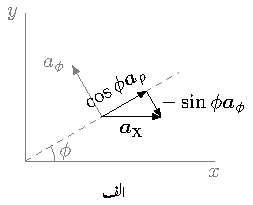
\includegraphics{figVectorCartesianXtoCylindricalConversion}
\end{subfigure}%
%
\begin{subfigure}{0.4\textwidth}
\centering
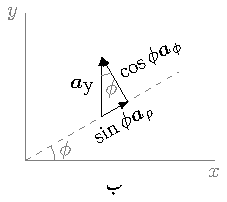
\includegraphics{figVectorCartesianYtoCylindricalConversion}
\end{subfigure}%
\caption{\عددیء{\ax} اور \عددیء{\ay} کا نلکی محدد میں تبادلہ۔}
\label{شکل_سمتیہ_نلکی_محدد_میں_کارتیسی_اکائی_سمتیات}
\end{figure}%

شکل \حوالہ{شکل_سمتیہ_نلکی_محدد_میں_کارتیسی_اکائی_سمتیات}-الف میں \عددیء{\ax} کا نلکی محدد میں تبادلہ دکھایا گیا ہے۔جس نقطے پر ایسا درکار ہو، اس نقطے پر \عددیء{\ax} کی دُم رکھیں۔مرکز سے نقطے تک نقطہ دار سیدھی لکیر کھینچتے ہوئے اسے مزید آگے بڑھائیں۔اس نقطے پر \عددیء{\arho} اسی لکیر کی سمت میں ہو گا جبکہ \عددیء{\aphi} لکیر کے ساتھ نوے درجے کا زاویہ بنائے گا۔شکل میں \عددیء{\aphi} دکھایا گیا ہے۔جیسا شکل میں دکھایا گیا ہے، \عددیء{\ax} کی نوک سے نقطہ دار لکیر پر عمود بنائیں۔صاف ظاہر ہے کہ \عددیء{\ax} کو دو عدد سمتیات کی مدد سے لکھا جا سکتا ہے۔ان میں سے ایک سمتیہ \عددیء{\arho} کی سمت میں اور دوسرا سمتیہ \عددیء{\aphi} کی الٹ جانب کو ہو گا۔یوں
\begin{align}\label{مساوات_سمتیہ_اکائی_ایکس_نلکی_میں}
\ax=\cos \phi \arho-\sin \phi \aphi
\end{align}
لکھا جا سکتا ہے۔شکل \حوالہ{شکل_سمتیہ_نلکی_محدد_میں_کارتیسی_اکائی_سمتیات}-ب میں \عددیء{\ay} کا نلکی محدد میں تبادلہ دکھایا گیا ہے۔یہاں نقطہ پر \عددیء{\ay} کی دُم رکھتے ہوئے اس کی نوک سے نقطہ دار لکیر پر عمود کھینچا گیا ہے۔یوں
\begin{align}\label{مساوات_سمتیہ_اکائی_وائے_نلکی_میں}
\ay=\sin \phi \arho+\cos \phi \aphi
\end{align}
لکھا جا سکتا ہے۔

آئیں مساوات \حوالہ{مساوات_سمتیہ_اکائی_رداس_کارتیسی_میں} تا مساوات \حوالہ{مساوات_سمتیہ_اکائی_وائے_نلکی_میں} کو جدول \حوالہ{جدول_سمتیہ_نلکی_کارتیسی_اکائی_غیر-سمتی_ضرب} کی مدد سے حاصل کریں۔کسی بھی سمتیہ \عددیء{\kvec{A}} کو کارتیسی یا نلکی محدد میں لکھا جا سکتا ہے۔یوں
\begin{gather}
\begin{aligned}\label{مساوات_سمتیہ_سمتیہ_نلکی_کارتیسی_اشکال}
\kvec{A}&=A_x \ax+A_y \ay+A_z\az\\
&=A_\rho \arho+A_\phi \aphi+A_z \az
\end{aligned}
\end{gather}
لکھا جا سکتا ہے۔ان میں پہلی مساوات کا باری باری \عددیء{\ax}، \عددیء{\ay} اور \عددیء{\az} کے ساتھ غیر سمتی ضرب لیتے ہوئے 
\begin{gather}
\begin{aligned}\label{مساوات_سمتیہ_کارتیسی_اجزاء}
\ax \cdot \kvec{A}&=A_x \ax \cdot \ax+A_y \ax \cdot \ay+A_z \ax \cdot \az=A_x\\
\ay \cdot \kvec{A}&=A_x \ay \cdot \ax+A_y \ay \cdot \ay+A_z \ay \cdot \az=A_y\\
\az \cdot \kvec{A}&=A_x \az \cdot \ax+A_y \az \cdot \ay+A_z \az \cdot \az=A_z
\end{aligned}
\end{gather}
حاصل ہوتے ہیں۔\عددیء{\kvec{A}} کو کارتیسی نظام میں لکھنے کی خاطر \عددیء{A_x}، \عددیء{A_y} اور \عددیء{A_z} درکار ہوتے ہیں جنہیں مندرجہ بالا مساوات سے حاصل کیا جا سکتا ہے۔اسی طرح مساوات \حوالہ{مساوات_سمتیہ_سمتیہ_نلکی_کارتیسی_اشکال} کے نچلے حصے کا باری باری \عددیء{\arho}، \عددیء{\aphi} اور \عددیء{\az} کے ساتھ غیر سمتی ضرب لیتے ہوئے
\begin{gather}
\begin{aligned}\label{مساوات_سمتیہ_نلکی_اجزاء}
\arho \cdot \kvec{A}&=A_\rho \arho \cdot \arho +A_\phi \arho \cdot \aphi +A_z \arho \cdot \az=A_\rho\\
\aphi \cdot \kvec{A}&=A_\rho \aphi \cdot \arho +A_\phi \aphi \cdot \aphi +A_z \aphi \cdot \az=A_\phi \\
\az \cdot \kvec{A}&=A_\rho \az \cdot \arho +A_\phi \az \cdot \aphi +A_z \az \cdot \az=A_z
\end{aligned}
\end{gather}
حاصل ہوتے ہیں۔یوں \عددیء{\kvec{A}} کو نلکی نظام میں لکھنے کی خاطر \عددیء{A_\rho}، \عددیء{A_\phi} اور \عددیء{A_z} کو مندرجہ بالا مساوات کی مدد سے حاصل کیا جا سکتا ہے۔

آئیں \عددیء{\arho} کو کارتیسی نظام میں لکھیں۔یوں \عددیء{\kvec{A}=\arho} کو  کارتیسی نظام میں لکھنا مطلوب ہے۔مساوات \حوالہ{مساوات_سمتیہ_کارتیسی_اجزاء} کے مطابق  \عددیء{A_x} حاصل کرنے کی خاطر \عددیء{\ax \cdot \kvec{A}} لینا ہو گا۔جدول \حوالہ{جدول_سمتیہ_نلکی_کارتیسی_اکائی_غیر-سمتی_ضرب} کے استعمال سے
\begin{align*}
A_x=\ax \cdot \kvec{A}=\ax \cdot \arho=\cos \phi
\end{align*}  
حاصل ہوتا ہے۔اسی طرح جدول کو استعمال کرتے ہوئے
\begin{align*}
A_y=\ay \cdot \kvec{A}=\ay \cdot \arho=\sin \phi
\end{align*}
اور 
\begin{align*}
A_z=\az \cdot \kvec{A}=\az \cdot \arho=0
\end{align*}
حاصل کرتے  ہیں۔یوں کارتیسی نظام میں \عددیء{\kvec{A}=A_x\ax+A_y\ay+A_z\az} لکھتے ہوئے
\begin{align*}
\arho = \cos \phi \ax +\sin \phi \ay
\end{align*}
لکھا جائے گا۔ یہی جواب مساوات \حوالہ{مساوات_سمتیہ_اکائی_رداس_کارتیسی_میں} میں بھی حاصل کیا گیا تھا۔

\عددیء{\aphi} کو بھی اسی طرح کارتیسی نظام میں لکھا جا سکتا ہے۔ایسا کرنے کی خاطر جدول \حوالہ{جدول_سمتیہ_نلکی_کارتیسی_اکائی_غیر-سمتی_ضرب} کی مدد سے  اس سمتیہ کا باری باری \عددیء{\ax}، \عددیء{\ay} اور \عددیء{\az} کے ساتھ غیر سمتی ضرب لیتے ہیں۔
\begin{align*}
A_x&=\ax \cdot \aphi=-\sin \phi\\
A_y&=\ay \cdot \aphi=\cos \phi\\
A_z&=\az \cdot \aphi=0
\end{align*}
یوں
\begin{align*}
\aphi=A_x \ax+A_y \ay+A_z \az = -\sin \phi \ax+\cos \phi \ay
\end{align*}
حاصل ہوتا ہے۔یہی جواب مساوات \حوالہ{مساوات_سمتیہ_اکائی_زاویہ_کارتیسی_میں} بھی دیتا ہے۔

آپ سے گزارش ہے کہ جدول \حوالہ{مساوات_سمتیہ_اکائی_زاویہ_کارتیسی_میں} کو یاد کرنے کی کوشش نہ کریں۔اپنے آپ میں یہ صلاحیت پیدا کریں کہ ان جوابات کو آپ جلد اخذ کر سکیں۔

\ابتدا{مشق}
\عددیء{\ax}، \عددیء{\ay} اور \عددیء{\az} کو جدول \حوالہ{جدول_سمتیہ_نلکی_کارتیسی_اکائی_غیر-سمتی_ضرب} کی مدد سے  نلکی محدد میں لکھیں۔

جوابات:
\begin{align*}
\ax&=\cos \phi \arho-\sin \phi \aphi\\
\ay&=\sin \phi \arho+\cos \phi \aphi\\
\az&=\az
\end{align*}
\انتہا{مشق}
%
\begin{figure}
\centering
\begin{subfigure}{0.4\textwidth}
\centering
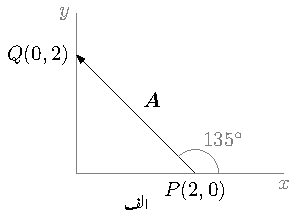
\includegraphics{figVectorVectorInCartesianAndCylindricalA}
\end{subfigure}%
%
\begin{subfigure}{0.4\textwidth}
\centering
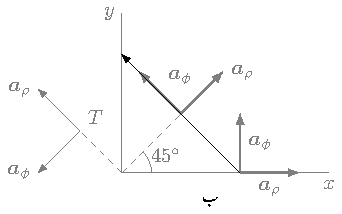
\includegraphics{figVectorVectorInCartesianAndCylindricalB}
\end{subfigure}%
\caption{کارتیسی اور نلکی محدد میں سمتیہ۔}
\label{شکل_سمتیہ_کارتیسی_نلکی_مساوات}
\end{figure}

شکل \حوالہ{شکل_سمتیہ_کارتیسی_نلکی_مساوات} میں \عددیء{P(2,0)} سے \عددیء{Q(0,2)} تک سمتیہ \عددیء{\kvec{A}} دکھایا گیا ہے۔کارتیسی نظام میں 
\begin{align}\label{مساوات_سمتیہ_کارتیسی_نظام_سمتیہ_مثال}
\kvec{A}&=-2\ax+2\ay
\end{align}
لکھا جا سکتا ہے۔اس سمتیہ کی حتمی قیمت
\begin{align*}
\abs{\kvec{A}}= \sqrt{\kvec{A} \cdot \kvec{A}}=\sqrt{(-2\ax+2\ay) \cdot (-2\ax+2\ay)}=\sqrt{8}
\end{align*}
ہے۔آئیں اسی سمتیہ کو نلکی محدد میں لکھیں۔ایسا کرنے کی خاطر \عددیء{A_\rho} اور \عددیء{A_\phi} درکار ہوں گے جنہیں حاصل کرنے کی خاطر جدول \حوالہ{جدول_سمتیہ_نلکی_کارتیسی_اکائی_غیر-سمتی_ضرب}  کی مدد سے \عددیء{\arho \cdot \kvec{A}} اور \عددیء{\aphi \cdot \kvec{A}} حاصل کرتے ہیں۔
\begin{align*}
A_\rho&=\arho \cdot (-2\ax+2\ay)=-2 \cos \phi +2 \sin \phi\\
A_\phi&=\aphi \cdot  (-2\ax+2\ay)=2 \sin \phi +2 \cos \phi
\end{align*}
یوں
\begin{align}\label{مساوات_سمتیہ_نلکی_نظام_سمتیہ_مثال}
\kvec{A}=2(- \cos \phi + \sin \phi) \arho +2( \sin \phi + \cos \phi)\aphi
\end{align}
لکھا جا سکتا ہے۔آئیں دیکھیں کہ اس کی حتمی قیمت کیا حاصل ہوتی ہے۔اکائی سمتیات کا غیر سمتی ضرب \عددیء{\arho \cdot \arho=1}، \عددیء{\aphi \cdot \aphi=1} اور \عددیء{\arho \cdot \aphi=0} استعمال کرتے ہوئے
\begin{align*}
\abs{\kvec{A}}&=\sqrt{\kvec{A} \cdot \kvec{A}}\\
&=\sqrt{2^2(- \cos \phi + \sin \phi)^2+2^2( \sin \phi + \cos \phi)^2 }\\
&=\sqrt{4(\cos^2 \phi +\sin^2 \phi -2 \cos \phi \sin \phi)+4(\cos^2 \phi +\sin^2 \phi +2 \cos \phi \sin \phi)}\\
&=\sqrt{8(\cos^2 \phi+\sin^2 \phi)}\\
&=\sqrt{8}
\end{align*}
حاصل ہوتا ہے جہاں آخری قدم پر \عددیء{\cos^2 \alpha+\sin^2 \alpha=1} کا استعمال کیا گیا ہے۔یقیناً سمتیہ کی حتمی قیمت محدد کے نظام پر منحصر نہیں۔

مساوات \حوالہ{مساوات_سمتیہ_کارتیسی_نظام_سمتیہ_مثال} اور مساوات \حوالہ{مساوات_سمتیہ_نلکی_نظام_سمتیہ_مثال} ایک ہی سمتیہ کو لکھنے کے دو طریقے ہیں۔یہاں کارتیسی نظام کا استعمال نہایت آسان ثابت ہوا۔ آگے چل کر آپ دیکھیں گے کہ کہیں مسئلوں میں نلکی محدد کا استعمال زیادہ آسان ہو گا۔آئیں مساوات \حوالہ{مساوات_سمتیہ_کارتیسی_نظام_سمتیہ_مثال} پر مزید غور کریں۔اس مساوات میں اکائی سمتیات از خود اٹل نہیں ہیں۔ان کی سمتوں کا دارومدار زاویہ \عددیء{\phi} پر ہے۔شکل  \حوالہ{شکل_سمتیہ_کارتیسی_نلکی_مساوات}-ب میں \عددیء{\phi=0^\circ}، \عددیء{\phi=45^\circ} اور \عددیء{\phi=135^\circ} پر \عددیء{\arho} اور \عددیء{\aphi} دکھائے گئے ہیں۔نقطہ \عددیء{P} یعنی \عددیء{\phi=0^\circ} پر مساوات \حوالہ{مساوات_سمتیہ_نلکی_نظام_سمتیہ_مثال} 
\begin{align*}
\kvec{A}_{ \phi=0^\circ}&=2(- \cos 0^\circ + \sin 0^\circ ) \arho +2( \sin 0^\circ  + \cos 0^\circ )\aphi\\
&=-2\arho+2\aphi 
\end{align*} 
صورت اختیار کر لیتی ہے۔اس مساوات کے مطابق \عددیء{\phi=0^\circ} پر \عددیء{\kvec{A}} کو دو عدد سمتیات کے مجموعہ کی صورت میں لکھا جا سکتا ہے جن میں پہلی سمتیہ \عددیء{\arho} کے الٹ سمت میں ہے اور اس کی لمبائی دو کے برابر ہے جبکہ دوسری سمتیہ کی مقدار دو اور اس کی سمت \عددیء{\aphi} کی سمت میں ہی ہے۔\حوالہ{شکل_سمتیہ_کارتیسی_نلکی_مساوات}-ب میں نقطہ \عددیء{P} پر \عددیء{\kvec{A}} کی سمت واقع بڑھتی \عددیء{\aphi} اور گھٹتی \عددیء{\arho} کی سمت میں ہے۔یاد رہے کہ اس مساوات میں \عددیء{\arho} اور \عددیء{\aphi} کو \عددیء{\phi=0^\circ} پر حاصل کیا گیا ہے۔\عددیء{\phi=0^\circ} پر \عددیء{\arho} اور \عددیء{\ax} برابر ہوتے ہیں اور اسی طرح \عددیء{\aphi} اور \عددیء{\ay} برابر ہوتے ہیں۔یہی وجہ ہے کہ مساوات \حوالہ{مساوات_سمتیہ_کارتیسی_نظام_سمتیہ_مثال} میں \عددیء{\ax} کی جگہ \عددیء{\arho} اور \عددیء{\ay} کی جگہ \عددیء{\aphi} پُر کرنے سے مندرجہ بالا مساوات لکھی جا سکتی ہے۔

\عددیء{\phi=45^\circ} پر مساوات \حوالہ{مساوات_سمتیہ_نلکی_نظام_سمتیہ_مثال}
\begin{align*}
\kvec{A}_{\phi=45^\circ}&=2(- \cos 45^\circ + \sin 45^\circ ) \arho +2( \sin 45^\circ  + \cos 45^\circ )\aphi\\
&=2(- \frac{1}{\sqrt{2}} +\frac{1}{\sqrt{2}} ) \arho +2( \frac{1}{\sqrt{2}}  + \frac{1}{\sqrt{2}} )\aphi\\
&=\sqrt{8} \aphi
\end{align*} 
صورت اختیار کر لیتی ہے۔اس مساوات کے مطابق \عددیء{\phi=45^\circ} پر \عددیء{\kvec{A}} صرف اور صرف \عددیء{\aphi} کی سمت میں ہے اور اس کی لمبائی \عددیء{\sqrt{8}} ہے۔شکل \حوالہ{شکل_سمتیہ_کارتیسی_نلکی_مساوات}-ب میں یہ حقیقت واضح ہے کہ \عددیء{\phi=45^\circ}  پر \عددیء{\kvec{A}} کی سمت \عددیء{\aphi} ہی ہے۔یاد رہے کہ اس مساوات میں \عددیء{\arho} اور \عددیء{\aphi} کو \عددیء{\phi=45^\circ} پر حاصل کیا گیا ہے۔شکل میں اکائی سمتیات کو عین \عددیء{\kvec{A}} کے اوپر کھینچا گیا ہے تا کہ سمتیات کی سمتوں کا موازنہ آسانی سے کیا جا سکے۔

آپ نے دیکھا کہ نلکی محدد میں سمتیہ کی مساوات کا دارومدار اس نقطے پر ہے جس نقطے کے اکائی سمتیات استعمال کئے جائیں۔آئیں دیکھیں کہ \عددیء{\phi=135^\circ} پر پائے جانے والے  نقطہ \عددیء{T} کے اکائی سمتیات استعمال کرتے ہوئے \عددیء{\kvec{A}} کیسا لکھا جائے گا۔مساوات \حوالہ{مساوات_سمتیہ_نلکی_نظام_سمتیہ_مثال} میں \عددیء{\phi=135^\circ} پُر کرنے سے
\begin{align*}
\kvec{A}_{\phi=135^\circ}&=2(- \cos 135^\circ + \sin 135^\circ) \arho +2( \sin 135^\circ + \cos 135^\circ)\aphi\\
&=2(\frac{1}{\sqrt{2}}+\frac{1}{\sqrt{2}})\arho+2(\frac{1}{\sqrt{2}}-\frac{1}{\sqrt{2}})\aphi\\
&=\sqrt{8}\arho
\end{align*}
حاصل ہوتا ہے۔اس مساوات کے مطابق \عددیء{\phi=135^\circ} کے اکائی سمتیات استعمال کرتے ہوئے \عددیء{\kvec{A}} کو \عددیء{\arho} کی سمت میں \عددیء{\sqrt{8}} لمبائی کا سمتیہ لکھا جا سکتا ہے۔شکل سے یہ حقیقت واضح ہے۔ 

\begin{figure}
\centering
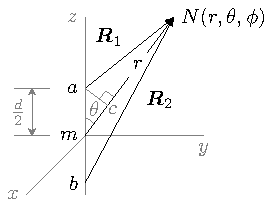
\includegraphics{figVectorDipole}
\caption{جفت قطب کے برقی بار سے دور نقطے تک فاصلے۔}
\label{شکل_سمتیہ_جفت_قطب}
\end{figure}
%================
\ابتدا{مثال}\شناخت{مثال_سمتیہ_جفت_قطب}
شکل \حوالہ{شکل_سمتیہ_جفت_قطب} میں \عددیء{z} محدد پر نقطہ \عددیء{a(0,0,\tfrac{d}{2})} پر مثبت \اصطلاح{برقی بار}\فرہنگ{برقی بار}\فرہنگ{بار!برقی}\فرہنگ{برق}\حاشیہب{electric charge}\فرہنگ{charge} \عددیء{+Q} اور نقطہ \عددیء{b(0,0,-\tfrac{d}{2})} پر منفی برقی بار  \عددیء{-Q} پائے جاتے ہیں۔ایسے دو برابر لیکن الٹ علامت کے دو قریب قریب پائے جانے والے برقی باروں کے جوڑی کو \اصطلاح{جفت قطب}\فرہنگ{جفت قطب}\حاشیہب{dipole}\فرہنگ{dipole} کہتے ہیں۔دکھائے گئے سمتی فاصلوں \عددیء{\kvec{R}_1} اور \عددیء{\kvec{R}_2} کو کروی محدد میں لکھیں۔ 

حل:\عددیء{m} سے \عددیء{N} تک فاصلہ \عددیء{r} ہے اور اس سمت میں اکائی سمتیہ \عددیء{\ar} ہے۔نقطہ \عددیء{a} سے  \عددیء{r} پر عمودی لکیر لگائی گئی ہے جو اسے \عددیء{c} پر ملتی ہے۔یوں \عددیء{ac} کی سمت کروی محدد کے اکائی سمتیہ \عددیء{\atheta} کی سمت میں ہے۔شکل کو دیکھتے ہوئے \عددیء{mc=\tfrac{d}{2} \cos \theta} اور \عددیء{ac=\tfrac{d}{2} \sin \theta} لکھے جا سکتے ہیں۔یوں \عددیء{\kvec{R}_1} کو ہم \عددیء{a} سے \عددیء{c} تک سمتیہ \عددیء{\tfrac{d}{2} \sin \theta \atheta} اور \عددیء{c} سے \عددیء{N} تک سمتیہ \عددیء{(r-\tfrac{d}{2}\cos \theta)\ar} کے مجموعے کی شکل میں 
\begin{align}
\kvec{R}_1=\frac{d}{2}\sin\theta \atheta+(r-\frac{d}{2}\cos\theta)\ar
\end{align}
 لکھ سکتے ہیں۔ہم اسی طرح شکل \حوالہ{شکل_سمتیہ_جفت_قطب} میں \عددیء{N} سے \عددیء{m} تک لکیر کو \عددیء{m} سے آگے بڑھا کر \عددیء{b} سے اس پر عمودی لکیر کھینچ کر شکل کو دیکھتے ہوئے  \عددیء{\kvec{R}_2} کی مساوات بھی لکھ سکتے ہیں البتہ ایسا کرنے کی بجائے آئیں \عددیء{\kvec{R}_2} کی مساوات تحلیلی طریقے سے حاصل کریں۔شکل کو دیکھتے ہوئے
\begin{align*}
\kvec{R}_2=\frac{d}{2} \az+r\ar
\end{align*}
لکھا جا سکتا ہے جہاں کارتیسی محدد کی اکائی سمتیہ \عددیء{\az} اور کروی محدد کی اکائی سمتیہ \عددیء{\ar} استعمال کئے گئے۔کروی محدد میں کسی بھی لکیر کی طرح 
\begin{align*}
\kvec{R}_2=A_r \ar+A_\theta \atheta+A_\phi \aphi
\end{align*}
لکھا جا سکتا ہے۔آئیں \عددیء{A_r=\kvec{R}_2 \cdot \ar} سے حاصل کریں۔
\begin{align*}
A_r =\left(\frac{d}{2} \az+r\ar \right) \cdot \ar=\frac{d}{2}\cos \theta+r
\end{align*}
اسی طرح \عددیء{A_\theta=\kvec{R}_2 \cdot \atheta} سے حاصل کرتے ہیں۔
\begin{align*}
A_\theta =\left(\frac{d}{2} \az+r\ar \right) \cdot \atheta=-\frac{d}{2}\sin \theta
\end{align*}
اسی طرح \عددیء{A_\phi=\kvec{R}_2 \cdot \aphi} لکھتے ہوئے \عددیء{A_\phi=0} حاصل ہوتا ہے۔یوں
\begin{align}
\kvec{R}_2=\left(\frac{d}{2}\cos \theta+r \right)\ar-\frac{d}{2}\sin \theta \atheta
\end{align}
لکھا جا سکتا ہے۔
\انتہا{مثال}
%
\begin{figure}
\centering
\begin{subfigure}{0.5\textwidth}
\centering
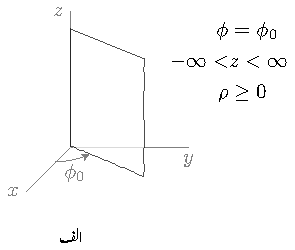
\includegraphics{figVectorCylindricalFixedAngleSurface}
\end{subfigure}%
%
\begin{subfigure}{0.5\textwidth}
\centering
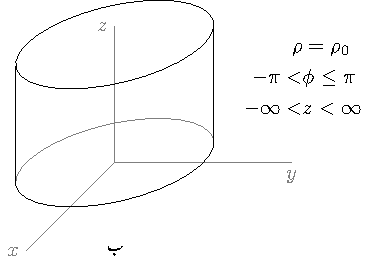
\includegraphics{figVectorCylindricalFixedRadiusSurface}
\end{subfigure}%
\caption{$\phi=\phi_0$ اور $\rho=\rho_0$ سطحیں۔}
\label{شکل_سمتیہ_نلکی_قطعی_زاویہ_سطح}
\end{figure}
\جزوحصہ{نلکی لامحدود سطحیں}
شکل \حوالہ{شکل_سمتیہ_نلکی_قطعی_زاویہ_سطح}-الف میں \عددیء{\phi} تبدیل کئے بغیر \عددیء{\rho} اور \عددیء{z} کی قیمتیں تبدیل کرتے ہوئے \عددیء{\phi=\phi_0} سطح کا حصول دکھایا گیا ہے۔یہ سطح نلکی شکل رکھتی ہے  جس کا اوپر والا منہ اور نچلا منہ کھلے ہیں یعنی ان پر ڈھکن نہیں۔شکل-ب میں \عددیء{\rho} تبدیل کئے بغیر \عددیء{\phi} اور \عددیء{z} کو تبدیل کرتے ہوئے \عددیء{\rho=\rho_0} سطح کا حصول دکھایا گیا ہے۔ان دونوں لامحدود سطحوں کے کچھ حصے ان  اشکال میں  دکھائے گئے ہیں۔ شکل-الف میں \عددیء{\rho} کی قیمت صرف مثبت جبکہ \عددیء{z} کی قیمت مثبت یا منفی ممکن ہے۔شکل-ب میں زاویہ کُل \عددیء{2\pi} ریڈیئن تبدیل ہو سکتا ہے۔یوں زاویے کا مثبت حد \عددیء{\pi} ریڈیئن یعنی \عددیء{180} درجہ ہے جبکہ اس کا منفی\حاشیہد{حقیقت میں منفی حد \عددیء{-180^\circ} کو نہیں چھوتا۔اگر منفی حد \عددیء{-180^\circ} کو چھوئے تب منفی \عددیء{x} محدد دو مرتبہ شامل ہوتا ہے۔} حد \عددیء{-\pi} یعنی \عددیء{-180} درجے ہے۔نلکی محدد اور کارتیسی نظام دونوں میں \عددیء{z=z_0}  سطح یکساں بنتی ہے۔

جیسے شکل \حوالہ{شکل_سمتیہ_نلکی_تین_سطحیں} میں دکھایا گیا ہے، \عددیء{\rho=\rho_1} اور \عددیء{\phi=\phi_1}  سطحیں \عددیء{\az} کی سیدھ میں سیدھی لکیر پر ملتے ہیں۔اسی طرح \عددیء{\rho=\rho_1} اور \عددیء{z=z_1} سطحیں ایک گول دائرے پر ملتے ہیں جبکہ \عددیء{\phi=\phi_1} اور \عددیء{z=z_1} سطحیں \عددیء{\arho} کی سیدھ میں سیدھی لکیر پر ملتے ہیں۔\عددیء{\rho=\rho_1}، \عددیء{\phi=\phi_1} اور \عددیء{z=z_1} سطحیں صرف اور صرف ایک ہی نقطہ \عددیء{N} پر اکٹھے ملتے ہیں۔نلکی محدد میں کسی بھی نقطے  کا مقام اسی طرح تین سطحوں کے  متقاطع نقطہ سے حاصل کیا جاتا ہے البتہ \عددیء{(0,0,z)} تک پہنچنے کی خاطر ایسا کرنے کی ضرورت نہیں ہوتی۔

\begin{figure}
\centering
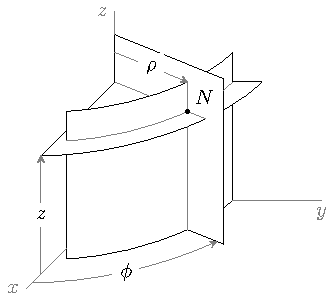
\includegraphics{figVectorCylindricalIntersectingSurfaces}
\caption{نلکی محدد کے تین سطحیں۔}
\label{شکل_سمتیہ_نلکی_تین_سطحیں}
\end{figure}
کسی بھی نقطہ \عددیء{N(\rho_1,\phi_1,z_1)} پر \عددیء{\rho=\rho_1}، \عددیء{\phi=\phi_1} اور \عددیء{z=z_1} سطحیں  بنانے کے بعد اگر نلکی محدد کے متغیرات کو \عددیء{\dif \rho}، \عددیء{\dif \phi} اور \عددیء{\dif z} بڑھا کر مزید تین سطحیں کھینچے جائیں تو یہ چھ سطحیں مل کر منحرف مکعب کو گھیریں گے جسے شکل \حوالہ{شکل_سمتیہ_نلکی_چھوٹی_حجم}-الف میں دکھایا گیا ہے۔رداسی سمت میں اس منحرف مکعب کے اطراف کی لمبائی \عددیء{\dif \rho} جبکہ \عددیء{\az}  سمت کے اطراف کی لمبائی \عددیء{\dif z} ہے۔ \عددیء{\aphi} سمت میں \عددیء{z} محدد کے قریبی  گول طرف کی لمبائی \عددیء{\rho \dif \phi} جبکہ محدد سے دور طرف کی گول لمبائی \عددیء{(\rho+\dif \rho)\dif \phi} ہے۔جیسے جیسے اس منحرف مکعب کو چھوٹا کیا جائے ویسے ویسے یہ ایک درست مکعب کی صورت اختیار کرتا ہے لہٰذا نہایت چھوٹے حجم کو مکعب تصور کرتے ہوئے اس کا حجم \عددیء{\rho \dif \rho \dif \phi \dif z} لکھا جا سکتا ہے۔
\begin{figure}
\centering
\begin{subfigure}{0.5\textwidth}
\centering
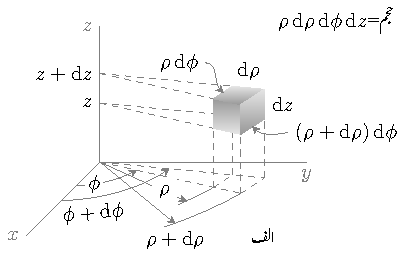
\includegraphics{figVectorCylindricalDifferentialVolume}
\end{subfigure}%
%
\begin{subfigure}{0.5\textwidth}
\centering
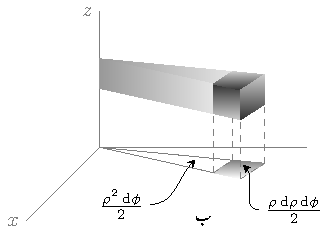
\includegraphics{figVectorCylindricalDifferentialTrapezium}
\end{subfigure}%
\caption{نلکی محدد میں انتہائی چھوٹی حجم۔}
\label{شکل_سمتیہ_نلکی_چھوٹی_حجم}
\end{figure}  

شکل \حوالہ{شکل_سمتیہ_نلکی_چھوٹی_حجم}-ب میں چھوٹے منحرف مکعب کو رداسی سمت میں \عددیء{z} محدد تک بڑھا کر پچر یا فانہ کی شکل میں دکھایا گیا ہے۔\عددیء{z=0} سطح پر اس کا عمودی سایہ بھی دکھایا گیا ہے۔\عددیء{\rho} رداس کے گول دائرے  کے مرکز سے  \عددیء{\dif \phi} زاویے پر دو لکیریں دائرے تک کھینچنے سے  \عددیء{\tfrac{\rho^2 \dif \phi}{2}} رقبہ گھیرا جاتا ہے۔اگر رداس \عددیء{\rho+\dif \rho} ہو تب رقبہ \عددیء{\tfrac{(\rho+\dif \rho)^2 \dif \phi}{2}} ہو گا۔یوں شکل-ب میں چھوٹے مکعب کے سایہ  کا رقبہ \عددیء{\dif S}
\begin{align*}
\dif S&=\frac{(\rho+\dif \rho)^2 \dif \phi}{2} - \frac{\rho^2 \dif \phi}{2}\\
&=\frac{\rho^2 \dif \phi +2 \rho \dif \rho \dif \phi+(\dif \rho)^2 \dif \phi}{2}-\frac{\rho^2 \dif \phi}{2}\\
&=\rho \dif \rho \dif \phi+\frac{(\dif \rho)^2 \dif \phi}{2}\\
&\approx \rho \dif \rho \dif \phi
\end{align*}
ہو گا۔یہاں آخری قدم پر \عددیء{\dif} کی علامت، مجموعہ کے پہلے رکن میں دو مرتبہ  جبکہ دوسرے رکن میں تین مرتبہ ہے۔یوں دوسرے اور پہلے رکن کی نسبت
  \عددیء{\tfrac{0.5(\dif \rho)^2 \dif \phi}{\rho \dif \rho \dif \phi}=\tfrac{\dif \rho}{2\rho}} ہو گی۔\عددیء{\dif \rho} کو کم سے کم\حاشیہد{کسی بھی متغیرہ مثلاً \عددیء{\rho} میں چھوٹی سی تبدیلی کو \عددیء{\Delta \rho} لکھا جاتا ہے جبکہ اس میں کم سے کم تبدیلی کو \عددیء{\dif \rho} لکھا 
جاتا ہے۔\عددیء{\dif \rho} کو تقریباً صفر سمجھا جا سکتا ہے یعنی \عددیء{\dif \rho \to 0} ہوتا ہے۔} کرتے ہوئے دوسرے رکن کو قابل نظر انداز بناتے ہوئے نظرانداز کیا گیا ہے۔یوں \عددیء{\rho \dif \rho \dif \phi} رقبہ اور \عددیء{\dif z} بلندی کے مکعب کا حجم \عددیء{\rho \dif \rho \dif \phi \dif z} ہو گا۔

شکل \حوالہ{شکل_سمتیہ_نلکی_چھوٹی_حجم} کو درست مکعب تصور کرتے ہوئے، اس کے اطراف کی لمبائی \عددیء{\rho \dif \phi}، \عددیء{\dif \rho} اور \عددیء{\dif z} لی جاتی ہے۔یوں مکعب کے نچلی اور اوپر سطح کا رقبہ مستطیل کے اطراف کو ضرب دیتے ہوئے  \عددیء{\rho \dif \rho \dif \phi} لکھا جا سکتا ہے۔اسی طرح سامنے اور پیچھے سطحوں  کا رقبہ \عددیء{\dif \rho \dif z} جبکہ بائیں اور دائیں سطحوں کا رقبہ \عددیء{\rho \dif \phi \dif z} لکھا جا سکتا ہے۔


شکل \حوالہ{شکل_سمتیہ_نلکی_چھوٹی_حجم}-الف میں نلکی محدد کے تینوں متغیرات تبدیل کرتے ہوئے ہم چھوٹے مکعب کے  \عددیء{N(\rho, \phi,z)} کونے سے \عددیء{N'(\rho+\dif \rho,\phi+\dif \phi,z+\dif z)} کونے پہنچتے ہیں۔\عددیء{N} سے \عددیء{N'} تک سمتیہ کو
\begin{align}\label{مساوات_سمتیہ_نلکی_چھوٹا_فاصلہ}
\dif \kvec{L}=\dif \rho \arho+\rho \dif \phi \aphi+\dif z \az
\end{align}
لکھا جاتا ہے۔یہ مساوات کسی بھی دو قریبی نقطوں کے مابین سمتی فاصلے کو ظاہر کرتی ہے۔

\حصہ{کروی محدد}
سیدھی لکیروں اور سیدھی سطحوں کو کارتیسی محدد میں زیادہ آسانی سے ظاہر کیا جا سکتا ہے جبکہ نلکی سطحوں کو ظاہر کرنے کے لئے نلکی محدد بہتر ثابت ہوتا ہے۔اسی طرح کرہ اشکال کے سطحوں کو کروی محدد میں باآسانی لکھا جا سکتا ہے۔آئیں کروی نظام پر غور کریں۔

شکل \حوالہ{شکل_سمتیہ_کروی_محدد_متغیرات}-الف میں کروی محدد کے متغیرات \عددیء{r}، \عددیء{\theta} اور \عددیء{\phi} دکھائے گئے ہیں۔محدد کے مرکز سے نقطہ \عددیء{N} تک کے فاصلے \عددیء{r} کو کروی رداس پکارا جاتا ہے جبکہ \عددیء{z} محدد سے کروی رداس تک زاویے کو \عددیء{\theta} لکھا جاتا ہے۔\عددیء{x} محدد سے رداس کے عمودی سائے تک زاویہ \عددیء{\phi} ہے۔کروی اور نلکی نظام میں \عددیء{\phi} یکساں بیان کیا جاتا ہے۔رداس کی  قیمت مثبت لی جاتی ہے۔یوں \عددیء{r \ge 0} ممکن ہے۔\عددیء{\theta} کی کم سے کم قیمت \عددیء{0^\circ} اور  زیادہ سے زیادہ  قیمت \عددیء{180^\circ} ہے جبکہ \عددیء{\phi} کی کم سے کم قیمت \عددیء{0^\circ} اور زیادہ سے زیادہ قیمت \عددیء{360^\circ} ہے۔

\begin{figure}
\centering
\begin{subfigure}{0.4\textwidth}
\centering
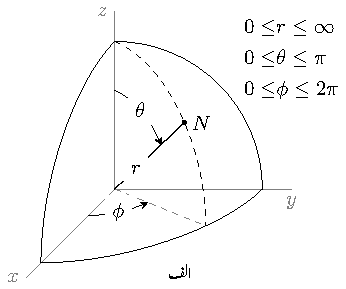
\includegraphics{figVectorSphericalRadiusThetaPhi}
\end{subfigure}%
%
\begin{subfigure}{0.4\textwidth}
\centering
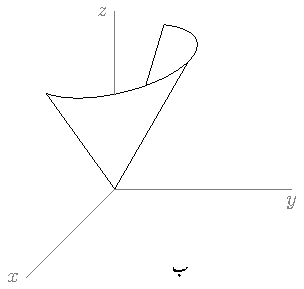
\includegraphics{figVectorSphericalThetaSurface}
\end{subfigure}%
\caption{(الف) کروی محدد کے متغیرات۔ (ب) \عددیء{\theta=\theta_0} سطح  کا کچھ حصہ۔}
\label{شکل_سمتیہ_کروی_محدد_متغیرات}
\end{figure}
%
\عددیء{r} اور \عددیء{\phi} تبدیل کئے بغیر \عددیء{\theta} کو \عددیء{0} سے بڑھاتے ہوئے \عددیء{\pi} ریڈیئن  کرنے سے نقطہ \عددیء{N}  شکل \حوالہ{شکل_سمتیہ_کروی_محدد_متغیرات}-الف میں نقطہ دار لکیر پر چلتے ہوئے  مثبت \عددیء{z} محدد سے شروع ہو کر  منفی \عددیء{z} محدد پر پہنچتا ہے۔اسے  نقطہ دار لکیر کو  کرہ ارض کے \اصطلاح{خط طول بلد}\فرہنگ{خط!طول بلد}\حاشیہب{longitude}\فرہنگ{longitude} تصور  کیا جا سکتا ہے۔  شکل-الف میں \عددیء{\theta} کا \عددیء{0^\circ} تا \عددیء{90^\circ} تبدیل ہوتا دکھایا گیا ہے۔اسی طرح \عددیء{r} اور \عددیء{\theta} تبدیل کئے بغیر \عددیء{\phi} کو \عددیء{0^\circ} تا \عددیء{360^\circ} تبدیل کرنے سے  نقطہ \عددیء{N} گول دائرے پر \عددیء{z} محدد کے گرد ایک چکر کاٹے گا۔یہ حرکت کرہ ارض کے \اصطلاح{خط عرض بلد}\فرہنگ{خط!عرض بلد}\حاشیہب{latitude}\فرہنگ{latitude} پر چلنے کے  مانند ہے۔\عددیء{\theta} اور \عددیء{\phi} تبدیل کئے بغیر \عددیء{r} کو تبدیل کرنے سے نقطہ \عددیء{N} مرکز سے  سیدھی باہر نکلتی لکیر پر حرکت کرتا ہے۔ 

\begin{figure}
\centering
\begin{subfigure}{0.5\textwidth}
\centering
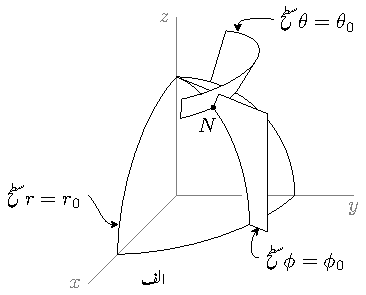
\includegraphics{figVectorSphericalIntersectingSurface}
\end{subfigure}%
%
\begin{subfigure}{0.5\textwidth}
\centering
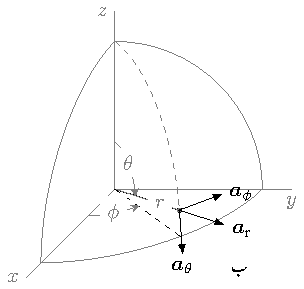
\includegraphics{figVectorSphericalUnitVectors}
\end{subfigure}%
\caption{(الف) تین عمودی سطحوں کے ملاپ سے نقطہ \عددیء{N} کا حصول۔ (ب) کروی محدد کے تین عمودی اکائی سمتیات۔}
\label{شکل_سمتیہ_کروی_تین_سطحوں_کا_ملاپ}
\end{figure}

\عددیء{r} تبدیل کئے بغیر \عددیء{\theta} کو \عددیء{0^\circ} تا \عددیء{180^\circ} اور \عددیء{\phi} کو \عددیء{0^\circ} تا \عددیء{360^\circ} تبدیل کرنے سے  نقطہ \عددیء{N} کروی \عددیء{r=r_0} سطح  پر حرکت کرے گا۔ اس کروی سطح کا رداس \عددیء{r} ہو گا۔شکل \حوالہ{شکل_سمتیہ_کروی_محدد_متغیرات}-الف  میں \عددیء{\theta} کو \عددیء{0^\circ} تا \عددیء{90^\circ} اور \عددیء{\phi} کو \عددیء{0^\circ} تا \عددیء{90^\circ} تبدیل کرنے سے حاصل سطح  دکھائی گئی ہے۔شکل \حوالہ{شکل_سمتیہ_کروی_محدد_متغیرات}-ب میں \عددیء{\theta} تبدیل کئے بغیر \عددیء{r} اور \عددیء{\phi} تبدیل کرنے سے پیدا مخروط\فرہنگ{مخروط}\حاشیہب{cone}\فرہنگ{cone}  \عددیء{\theta=\theta_0}  کروی سطح دکھائی گئی ہے۔\عددیء{\phi} تبدیل کئے بغیر \عددیء{r} اور \عددیء{\theta} تبدیل کرنے سے  نلکی محدد کی طرح \عددیء{\phi=\phi_0} سطح حاصل ہوتی ہے۔ شکل \حوالہ{شکل_سمتیہ_کروی_تین_سطحوں_کا_ملاپ}-الف میں ان تینوں سطحوں کو دکھایا گیا ہے۔بالکل کارتیسی اور نلکی محدد کی طرح، کسی بھی نقطہ \عددیء{N(r_0,\theta_0,\phi_0)} کا مقام ان تین سطحوں کے نقطہ ملاپ سے اخذ کیا جاتا ہے۔کسی بھی نقطہ \عددیء{N(r_0,\theta_0,\phi_0)} پر \عددیء{r=r_0}، \عددیء{\theta=\theta_0} اور \عددیء{\phi=\phi_0} سطحیں آپس میں عمودی ہوتی ہے اور یہ صرف اور صرف اسی نقطے پر اکٹھے ملتی ہیں۔

شکل \حوالہ{شکل_سمتیہ_کروی_تین_سطحوں_کا_ملاپ}-ب میں کروی نظام کے تین عمودی اکائی سمتیات \عددیء{\ar}، \عددیء{\atheta} اور \عددیء{\aphi} دکھائے گئے ہیں۔نلکی محدد کی طرح کروی محدد کے عمودی اکائی سمتیات بھی مقام تبدیل کرنے سے تبدیل ہوتے ہیں۔کسی بھی نقطہ \عددیء{N(r_0,\theta_0,\phi_0)} پر \عددیء{\theta} اور \عددیء{\phi} تبدیل کئے بغیر \عددیء{r} کے بڑھتے جانب اکائی سمتیہ \عددیء{\ar} ہو گی۔اسی طرح \عددیء{\theta} بڑھانے سے نقطہ \عددیء{N} اکائی سمتیہ \عددیء{\atheta} کی جانب حرکت کرے گا جبکہ \عددیء{\phi} بڑھانے سے نقطہ \عددیء{\aphi} کی جانب حرکت کرے گا۔کارتیسی اور نلکی محدد کی طرح کروی محدد کے اکائی سمتیات کو بھی محددی نظام کے متغیرات کو کم سے کم بڑھاتے ہوئے  نقطے کی حرکت کی جانب اکائی سمتیہ کھینچنے سے حاصل کیا جاتا ہے۔

شکل \حوالہ{شکل_سمتیہ_کروی_تین_سطحوں_کا_ملاپ}-الف سے واضح ہے کہ \عددیء{\ar} سمتیہ \عددیء{r=r_0} سطح کے عمودی جبکہ \عددیء{\theta=\theta_0} اور \عددیء{\phi=\phi_0} سطحوں کے متوازی ہے۔اسی طرح \عددیء{\atheta} سمتیہ \عددیء{\theta=\theta_0} سطح کے عمودی اور \عددیء{\phi=\phi_0} سطح کے متوازی پایا جاتا ہے جبکہ \عددیء{r=r_0} سطح کے ساتھ مماس بناتا ہے۔\عددیء{\aphi} سمتیہ \عددیء{\phi=\phi_0} سطح کے عمودی جبکہ \عددیء{r=r_0} اور \عددیء{\theta=\theta_0} سطحوں کے ساتھ مماس بناتا ہے۔

 
\عددیء{\ar}، \عددیء{\atheta} اور \عددیء{\aphi} کروی نظام  کے اکائی سمتیات ہیں۔\عددیء{\ar \times \atheta=\aphi} لکھنے سے  دائیں ہاتھ کا کروی نظام حاصل ہوتا ہے۔دائیں ہاتھ کے قانون میں دائیں ہاتھ کا انگوٹھا  \عددیء{r} جبکہ پہلی انگلی \عددیء{\theta}  اور دوسری انگلی \عددیء{\phi} بڑھانے سے پیدا حرکت کی سمتوں کو ظاہر کرتے ہیں۔نلکی محدد میں یہ انگلیاں \عددیء{\rho}، \عددیء{\phi} اور \عددیء{z} جبکہ کارتیسی محدد میں \عددیء{x}، \عددیء{y} اور \عددیء{z} بڑھانے سے پیدا حرکت کی سمتوں کو ظاہر کرتی ہیں۔

دائیں ہاتھ کے قانون  یا شکل \حوالہ{شکل_سمتیہ_کروی_صلیبی_ضرب_اکائی_سمتیات} کی مدد سے یوں اکائی سمتیات کے صلیبی ضرب
\begin{figure}
\centering
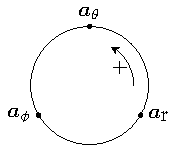
\includegraphics{figVectorSphericalRightHandCircle}
\caption{کروی نظام میں اکائی سمتیات کی صلیبی ضرب۔}
\label{شکل_سمتیہ_کروی_صلیبی_ضرب_اکائی_سمتیات}
\end{figure}

\begin{align}
\ar \times \atheta=\aphi \,\, , \quad \atheta \times \aphi=\ar \, \, , \quad \aphi \times \ar =\atheta
\end{align}

لکھے جا سکتے ہیں۔اسی طرح
\begin{align}
\ar \cdot \ar=1 \,\, , \quad \atheta \cdot \atheta=1 \,\, , \quad \aphi \cdot \aphi=1
\end{align}
اور
\begin{align}
\ar \cdot \atheta=0 \,\, , \quad \atheta \cdot \aphi=0 \,\, , \quad \aphi \cdot \ar=0
\end{align}
بھی لکھے جا سکتے ہیں۔

\begin{figure}
\centering
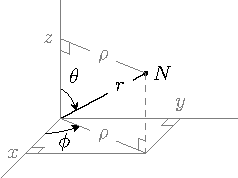
\includegraphics{figVectorSphericalToCylindricalAndCartesian}
\caption{کروی، نلکی اور کارتیسی متغیرات کا تبادلہ۔}
\label{شکل_سمتیہ_کروی_نلکی_متغیرات_تبادلہ}
\end{figure}

نقطہ \عددیء{N} کا \عددیء{z} محدد سے فاصلہ  \عددیء{\rho} ہے جو نلکی محدد کا رداس ہے۔اسے شکل \حوالہ{شکل_سمتیہ_کروی_نلکی_متغیرات_تبادلہ} میں دکھایا گیا ہے جہاں سے واضح ہے کہ \عددیء{\rho=r \sin \theta} کے برابر ہے۔اسی طرح \عددیء{z=0} سطح سے \عددیء{N} کی اونچائی \عددیء{z} ہے جو شکل کو دیکھتے ہوئے \عددیء{z=r\cos \theta}  لکھی جا سکتی ہے۔نقطہ \عددیء{N} کا عمودی سایہ \عددیء{z=0} سطح پر دکھایا گیا ہے جہاں سے واضح ہے کہ \عددیء{x=\rho \cos \phi} اور \عددیء{y=\rho \sin \phi} لکھے جا سکتے ہیں۔\عددیء{\rho=r \sin \theta} پُر کرنے سے درج ذیل لکھے جا سکتے ہیں
\begin{gather}
\begin{aligned}\label{مساوات_سمتیہ_کروی_سے_کارتیسی}
x&=r \sin \theta \cos \phi\\
y&=r \sin \theta \sin \phi\\
z&=r \cos \theta
\end{aligned}
\end{gather}
جہاں \عددیء{z} کی مساوات بھی ساتھ ہی لکھی  گئی ہے۔مساوات \حوالہ{مساوات_سمتیہ_کروی_سے_کارتیسی} کروی سے کارتیسی متغیرات دیتا ہے۔ اسی شکل کو دیکھتے ہوئے مسئلہ فیثاغورث کی مدد سے 
\begin{gather}
\begin{aligned}
r^2&=\rho^2+z^2\\
\rho^2&=x^2+y^2
\end{aligned}
\end{gather}
لکھتے ہوئے
\begin{align}\label{مساوات_سمتیہ_کروی_رداس}
r^2=x^2+y^2+z^2
\end{align}
حاصل ہوتا ہے۔مساوات \حوالہ{مساوات_سمتیہ_کروی_سے_کارتیسی} میں \عددیء{z} کی مساوات سے
\begin{align}\label{مساوات_سمتیہ_کروی_تھیٹا}
\theta = \cos^{-1} \frac{z}{r}=\cos^{-1}\frac{z}{\sqrt{x^2+y^2+z^2}}
\end{align}
 لکھا جا سکتا ہے۔اسی طرح  مساوات \حوالہ{مساوات_سمتیہ_کروی_سے_کارتیسی} کے \عددیء{y} کو \عددیء{x} سے تقسیم کرتے ہوئے
\begin{align}\label{مساوات_سمتیہ_کروی_فائے}
\phi = \tan^{-1} \frac{y}{x}
\end{align}
حاصل ہوتا ہے۔مساوات \حوالہ{مساوات_سمتیہ_کروی_رداس}، مساوات \حوالہ{مساوات_سمتیہ_کروی_تھیٹا} اور مساوات \حوالہ{مساوات_سمتیہ_کروی_فائے} کارتیسی سے کروی متغیرات دیتے ہیں۔
\begin{figure}
\centering
\begin{subfigure}{0.4\textwidth}
\centering
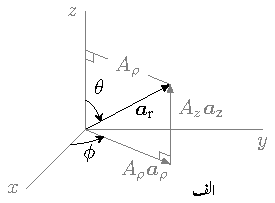
\includegraphics{figVectorSphericalUnitRadial}
\end{subfigure}%
%
\begin{subfigure}{0.4\textwidth}
\centering
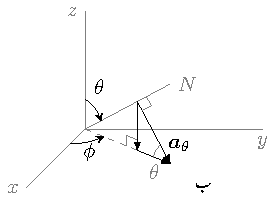
\includegraphics{figVectorSphericalUnitTheta}
\end{subfigure}%
\caption{کروی اکائی سمتیات کا کارتیسی نظام میں تبادلہ۔}
\label{شکل_سمتیہ_کروی_اکائی_رداسی_سمتیہ_کارتیسی}
\end{figure}

شکل \حوالہ{شکل_سمتیہ_کروی_تین_سطحوں_کا_ملاپ}-ب میں نقطہ \عددیء{N} پر اکائی سمتیات دکھائے گئے ہیں۔\عددیء{\ar} کی سمت تبدیل کئے بغیر اسے محدد کے مرکز پر منتقل کرتے ہوئے شکل \حوالہ{شکل_سمتیہ_کروی_اکائی_رداسی_سمتیہ_کارتیسی}-الف  میں دکھایا گیا ہے جہاں سے ظاہر ہے کہ اسے نلکی محدد کے اکائی سمتیات کی مدد سے
\begin{align}
\ar=A_\rho \arho+A_z \az
\end{align}
لکھا جا سکتا ہے۔شکل \حوالہ{شکل_سمتیہ_کروی_اکائی_رداسی_سمتیہ_کارتیسی}-الف  میں \عددیء{\ar} کی لمبائی ایک لیتے ہوئے  \عددیء{A_\rho=\sin \theta} اور \عددیء{A_z=\cos \theta} لکھا جا سکتا ہے۔یوں
\begin{align}\label{مساوات_سمتیہ_کروی_اکائی_نلکی_منتقل}
\ar=\sin \theta \arho+\cos \theta \az
\end{align}
حاصل ہوتا ہے۔اس مساوات کا باری باری \عددیء{\arho}، \عددیء{\aphi} اور \عددیء{\az} کے ساتھ غیر سمتی ضرب لیتے ہوئے
\begin{gather}
\begin{aligned}\label{مساوات_سمتیہ_کروی_رداس_نلکی_اکائی_غیر_سمتی_ضرب}
\ar \cdot \arho&=(\sin \theta \arho+\cos \theta \az) \cdot \arho=\sin \theta\\
\ar \cdot \aphi&=(\sin \theta \arho+\cos \theta \az) \cdot \aphi=0\\
\ar \cdot \az&=(\sin \theta \arho+\cos \theta \az) \cdot \az=\cos \theta
\end{aligned}
\end{gather}
حاصل ہوتا ہے جہاں \عددیء{\arho \cdot \arho=1}، \عددیء{\az \cdot \arho=0} وغیرہ کا استعمال کیا گیا۔یہ مساوات کروی رداسی اکائی سمتیے اور نلکی نظام کے اکائی سمتیات کے تمام ممکنہ غیر سمتی ضرب دیتا ہے۔اسی طرح جدول \حوالہ{جدول_سمتیہ_نلکی_کارتیسی_اکائی_غیر-سمتی_ضرب} استعمال کرتے ہوئے  مساوات  \حوالہ{مساوات_سمتیہ_کروی_اکائی_نلکی_منتقل} کا باری باری \عددیء{\ax} اور \عددیء{\ay} کے ساتھ غیر سمتی ضرب لیتے ہوئے
\begin{gather}
\begin{aligned}\label{مساوات_سمتیہ_کروی_رداس_کے_کارتیسی_اجزاء}
\ar \cdot \ax&=(\sin \theta \arho+\cos \theta \az) \cdot \ax=\sin \theta \cos \phi\\
\ar \cdot \ay&=(\sin \theta \arho+\cos \theta \az) \cdot \ay=\sin \theta \sin \phi\\
\ar \cdot \az&=(\sin \theta \arho+\cos \theta \az) \cdot \az=\cos \theta
\end{aligned}
\end{gather}
حاصل ہوتا ہے۔مکمل نتائج ایک جگہ لکھنے کی خاطر  مندرجہ بالا مساوات میں  \عددیء{\ar \cdot \az} کو بھی شامل کیا گیا ہے۔ یہ مساوات کروی اکائی رداسی  سمتیے  اور کارتیسی اکائی سمتیات کے تمام ممکنہ غیر سمتی ضرب دیتا ہے۔

\عددیء{\ar} کو کارتیسی نظام میں لکھنے کی خاطر \عددیء{\ar=\kvec{A}=A_x \ax+A_y \ay+A_z \az} لکھتے ہیں۔مساوات \حوالہ{مساوات_سمتیہ_کارتیسی_اجزاء} کے مطابق \عددیء{A_x=\ax \cdot \ar} جبکہ \عددیء{A_y=\ay \cdot \ar} اور \عددیء{A_z=\az \cdot \ar} ہوں گے۔یہ تمام  مساوات \حوالہ{مساوات_سمتیہ_کروی_رداس_کے_کارتیسی_اجزاء} میں دئے گئے ہیں۔ یوں 
\begin{align}
\ar=\sin \theta \cos \phi \ax+\sin \theta \sin \phi \ay+\cos \theta \az
\end{align}
لکھا جا سکتا ہے۔

شکل \حوالہ{شکل_سمتیہ_کروی_تین_سطحوں_کا_ملاپ}-ب میں دکھائے \عددیء{\atheta} کو \عددیء{\phi=\phi_0} سطح پر حرکت دیتے ہوئے  مرکز کے اتنے قریب لا کر شکل \حوالہ{شکل_سمتیہ_کروی_اکائی_رداسی_سمتیہ_کارتیسی}-ب میں دکھایا گیا ہے کہ اس کی نوک \عددیء{x=0} سطح کو چھوتی ہے۔جیسا شکل \حوالہ{شکل_سمتیہ_کروی_تین_سطحوں_کا_ملاپ}-الف سے واضح ہے،  \عددیء{\phi=\phi_0} سطح پر \عددیء{\atheta} کو حرکت دینے سے اس سمتیہ کی سمت تبدیل نہیں ہوتی۔شکل \حوالہ{شکل_سمتیہ_کروی_اکائی_رداسی_سمتیہ_کارتیسی}-ب کو دیکھتے ہوئے \عددیء{\atheta=B_\rho \arho-B_z \az} لکھا جا سکتا ہے۔یہاں رک کر  تسلی کر لیں کہ \عددیء{B_\rho \arho} اور \عددیء{\atheta} کے مابین زاویہ \عددیء{\theta} ہے۔\عددیء{\atheta}، \عددیء{B_\rho \arho} اور \عددیء{-B_z \az} مل کر تکون بناتے ہیں جسے دیکھتے ہوئے مسئلہ فیثاغورث کی مدد سے
\begin{align*}
B_\rho&=\cos \theta\\
B_z&=\sin \theta
\end{align*}
لکھا جا سکتا ہے۔یوں
\begin{align}\label{مساوات_سمتیہ_کروی_اکائی_تھیٹا}
\atheta=\cos \theta \arho-\sin \theta \az
\end{align}
کے برابر ہے۔اس مساوات کا باری باری \عددیء{\arho}، \عددیء{\aphi} اور \عددیء{\az} کے ساتھ غیر سمتی ضرب لینے سے
\begin{gather}
\begin{aligned}\label{مساوات_سمتیہ_کروی_تھیٹا_نلکی_اکائی_غیر_سمتی_ضرب}
\atheta \cdot \arho&=(\cos \theta \arho-\sin \theta \az) \cdot \arho=\cos \theta\\
\atheta \cdot \aphi&=(\cos \theta \arho-\sin \theta \az) \cdot \aphi=0\\
\atheta \cdot \az&=(\cos \theta \arho-\sin \theta \az) \cdot \az=-\sin \theta
\end{aligned}
\end{gather}
\عددیء{\atheta} اور نلکی اکائی سمتیات کے  تمام غیر سمتی ضرب حاصل ہوتے ہیں۔اسی طرح مساوات \حوالہ{مساوات_سمتیہ_کروی_اکائی_تھیٹا} کا باری باری \عددیء{ax}، \عددیء{\ay} اور \عددیء{\az} کے ساتھ غیر سمتی ضرب لینے سے
\begin{gather}
\begin{aligned}\label{مساوات_سمتیہ_کروی_تھیٹا_کے_کارتیسی_اجزاء}
\atheta \cdot \ax&=(\cos \theta \arho-\sin \theta \az) \cdot \ax=\cos \theta \arho \cdot \ax=\cos \theta \cos \phi\\
\atheta \cdot \ay&=(\cos \theta \arho-\sin \theta \az) \cdot \ay=\cos \theta \arho \cdot \ay=\cos \theta \sin \phi \\
\atheta \cdot \az&=(\cos \theta \arho-\sin \theta \az) \cdot \az=-\sin \theta \az \cdot \az=-\sin \theta
\end{aligned}
\end{gather}
حاصل ہوتے ہیں۔یہ مساوات \عددیء{\atheta} اور کارتیسی اکائی سمتیات کے تمام غیر سمتی ضرب دیتا ہے۔

\عددیء{\atheta} کو کارتیسی نظام میں لکھنے کی خاطر \عددیء{\atheta=\kvec{A}=A_x \ax+A_y\ay+A_z\az} لکھتے ہیں۔مساوات \حوالہ{مساوات_سمتیہ_کارتیسی_اجزاء} کے مطابق \عددیء{A_x=\ax \cdot \atheta} جبکہ \عددیء{A_y=\ay \cdot \atheta} اور \عددیء{A_z=\az \cdot \atheta} ہوں گے۔یہ تمام  مساوات \حوالہ{مساوات_سمتیہ_کروی_تھیٹا_کے_کارتیسی_اجزاء} میں دئے گئے ہیں۔ یوں
\begin{align}
\atheta=\cos \theta \cos \phi \ax+\cos \theta \sin \phi\ay-\sin \theta\az
\end{align}  
لکھا جا سکتا ہے۔

کروی  محدد کا \عددیء{\aphi} اور نلکی محدد کا \عددیء{\aphi} یکساں ہیں۔اسے کارتیسی نظام میں
\begin{align}
\aphi=-\sin \phi \ax+\cos \phi \ay
\end{align} 
لکھا جاتا ہے۔اس مساوات کا \عددیء{\ax}، \عددیء{\ay} اور \عددیء{\az} کے ساتھ غیر سمتی ضرب لیتے ہوئے
\begin{gather}
\begin{aligned}
\aphi \cdot \ax&=-\sin \phi\\
\aphi \cdot \ay&=\cos \phi\\
\aphi \cdot \az&=0
\end{aligned}
\end{gather}
لکھا جا سکتا ہے۔

مساوات \حوالہ{مساوات_سمتیہ_کروی_رداس_نلکی_اکائی_غیر_سمتی_ضرب} اور مساوات \حوالہ{مساوات_سمتیہ_کروی_تھیٹا_نلکی_اکائی_غیر_سمتی_ضرب} کے نتائج کے ساتھ \عددیء{\aphi} کے مختلف غیر سمتی ضربوں کو جدول \حوالہ{جدول_سمتیہ_کروی_نلکی_اکائی_غیر-سمتی_ضرب} میں یکجا کیا گیا ہے۔

\begin{table}
\caption{کروی  اکائی سمتیات کا نلکی اکائی سمتیات کے ساتھ غیر سمتی ضرب۔}
\centering
\begin{tabular}{l | r r r}
 & $\arho$ & $\aphi$ & $\az$ \\
\hline
$\ar$ & $\sin \theta$ & $0$& $\cos \theta$\\
$\atheta$ &$\cos \theta$ &$ 0$ &$ -\sin \theta$\\
$\aphi$ & $0$ &$ 1$ &$0$
\end{tabular}
\label{جدول_سمتیہ_کروی_نلکی_اکائی_غیر-سمتی_ضرب}
\end{table}
%

مساوات  \حوالہ{مساوات_سمتیہ_کروی_رداس_کے_کارتیسی_اجزاء} اور مساوات  \حوالہ{مساوات_سمتیہ_کروی_تھیٹا_کے_کارتیسی_اجزاء} کے نتائج جدول \حوالہ{جدول_سمتیہ_کروی_کارتیسی_اکائی_غیر-سمتی_ضرب} میں یکجا کئے گئے ہیں۔ 
\begin{table}
\caption{کروی  اکائی سمتیات کا کارتیسی اکائی سمتیات کے ساتھ غیر سمتی ضرب۔}
\centering
\begin{tabular}{l | r r r}
 & $\ax$ & $\ay$ & $\az$ \\
\hline
$\ar$ & $\sin \theta \cos \phi$ & $\sin \theta \sin \phi$& $\cos \theta$\\
$\atheta$ &$\cos \theta \cos \phi$ &$ \cos \theta \sin \phi$ &$ -\sin \theta$\\
$\aphi$ & $-\sin \phi$ &$ \cos \phi$ &$0$
\end{tabular}
\label{جدول_سمتیہ_کروی_کارتیسی_اکائی_غیر-سمتی_ضرب}
\end{table}
%
\begin{figure}
\centering
\begin{subfigure}{0.4\textwidth}
\centering
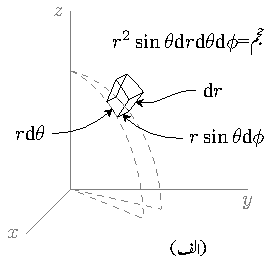
\includegraphics{figVectorSphericalDifferentialVolume}
\end{subfigure}%
%
\begin{subfigure}{0.4\textwidth}
\centering
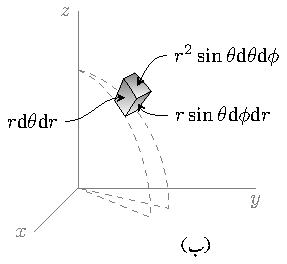
\includegraphics{figVectorSphericalDifferentialSurfaces}
\end{subfigure}%
\caption{(الف) کروی نظام میں  چھوٹی لمبائیاں اور چھوٹی حجم۔ (ب) کروی محدد میں چھوٹی سطحیں۔}
\label{شکل_سمتیہ_کروی_چھوٹی_حجم}
\end{figure}

شکل \حوالہ{شکل_سمتیہ_کروی_تین_سطحوں_کا_ملاپ} میں \عددیء{N(r,\theta,\phi)} پر تین عمودی سطحیں دکھائی گئی ہیں۔اگر کروی محدد کے متغیرات \عددیء{\dif r}، \عددیء{\dif \theta} اور \عددیء{\dif \phi} بڑھا کر دوبارہ تین عمودی سطحیں کھینچی جائیں تو یہ چھ سطحیں مل کر چھوٹا منحرف مکعب نما حجم گھیریں گی جسے شکل \حوالہ{شکل_سمتیہ_کروی_چھوٹی_حجم} میں دکھایا گیا ہے۔\عددیء{\ar} سمت میں مکعب کے چار اطراف کی لمبائیاں \عددیء{\dif r} ہے۔\عددیء{\atheta} سمت میں \عددیء{z} محدد کے قریبی دو اطراف کی لمبائیاں \عددیء{r \dif \theta} جبکہ دو دور اطراف کی لمبائیاں \عددیء{(r+\dif r)\dif \theta} ہے جسے دو اجزاء کی صورت میں یوں  \عددیء{r \dif \theta +\dif r \dif \theta} لکھا جا سکتا ہے۔دور اطراف کے لمبائی کا پہلا جزو ہوبہو قریبی اطراف کی لمبائی ہے جبکہ اس کا دوسرا جزو دور اور قریبی اطراف کے لمبائیوں میں فرق کو ظاہر کرتی ہے۔ان دو اجزاء کی نسبت \عددیء{\tfrac{\dif r \dif \theta}{r \dif \theta}=\tfrac{\dif r}{r}}  کے برابر ہے۔\عددیء{\dif r} کو کم سے کم\حاشیہد{کسی بھی متغیرہ مثلاً \عددیء{r} میں چھوٹی سی تبدیلی کو \عددیء{\Delta r} لکھا جاتا ہے جبکہ اس میں کم سے کم تبدیلی کو \عددیء{\dif r} لکھا جاتا ہے۔\عددیء{\dif r} کو تقریباً صفر سمجھا جا سکتا ہے یعنی \عددیء{\dif r \to 0} ہوتا ہے۔} کرتے ہوئے اس نسبت کو کم سے کم کیا جا سکتا  ہے۔ایسا ہی کرتے ہوئے ہم \عددیء{\dif r \dif \theta} کو رد کرتے ہوئے ان چاروں اطراف کی لمبائیاں \عددیء{r \dif \theta} ہی لیتے ہیں۔اسی طریقہ کار سے  \عددیء{\aphi} اطراف کی لمبائیاں  \عددیء{r \sin \theta \dif \phi} لکھی جا سکتی ہے۔منحرف مکعب نما کے اطراف میں معمولی فرق کو نظرانداز کرتے ہوئے اسے مکعب نما تصور کیا جا سکتا ہے جس کے \عددیء{r=r_0} سطحوں کا رقبہ \عددیء{r^2 \sin \theta \dif \theta \dif \phi} جبکہ \عددیء{\theta=\theta_0} سطحوں کا رقبہ \عددیء{r \sin \theta \dif r \dif \phi} اور \عددیء{\phi=\phi_0} سطحوں کا رقبہ   \عددیء{r \dif r \dif \theta} ہو گا۔اس مکعب کا حجم \عددیء{r^2 \sin \theta \dif r \dif \theta \dif \phi} ہو گا۔


شکل \حوالہ{شکل_سمتیہ_کروی_چھوٹی_حجم} میں کروی محدد کے تینوں متغیرات تبدیل کرتے ہوئے ہم چھوٹے مکعب کے  \عددیء{N(r,\theta,\phi)} کونے سے
 \عددیء{N'(r+\dif r,\theta+\dif \theta,\phi+\dif \phi)} کونے پہنچتے ہیں۔\عددیء{N} سے \عددیء{N'} تک سمتیہ کو
\begin{align}\label{مساوات_سمتیہ_کروی_چھوٹا_فاصلہ}
\dif \kvec{L}=\dif r \ar+r \dif \theta \atheta+r\sin \theta \dif \phi \aphi
\end{align}
لکھا جاتا ہے۔یہ مساوات کسی بھی دو قریبی نقطوں کے درمیان سمتی فاصلہ دیتا ہے۔

کسی بھی مکمل بند سطح کی  سمت، سطح کے عمودی باہر جانب لی جاتی ہے۔شکل \حوالہ{شکل_سمتیہ_کروی_چھوٹی_حجم} میں \عددیء{r=r_0} سطح  مرکز کا قریبی سطح ہے۔اس سطح کے دو آپس میں الٹ عمودی اطراف \عددیء{\mp \ar} ہیں جن میں \عددیء{-\ar} بند سطح کی بیرونی سمت کو ظاہر کرتا ہے لہٰذا یہی اس سطح کی درست سمت ہے۔اس کے برعکس \عددیء{r=r_0+\dif r} سطح مرکز سے دور تر ہے۔اس سطح کے بھی دو آپس میں الٹ عمودی سمتیں \عددیء{\mp \ar} ہیں جن میں \عددیء{\ar} سطح کی درست سمت ہے۔یوں  \عددیء{r=r_0} سطح کا سمتی رقبہ \عددیء{-r^2 \sin \theta \dif \theta \dif \phi \ar} جبکہ \عددیء{r=r_0+\dif r} سطح کا سمتی رقبہ \عددیء{\عددیء{r^2 \sin \theta \dif \theta \dif \phi \ar}} ہے۔اسی طرح \عددیء{\theta=\theta_0} سطح کا سمتی رقبہ \عددیء{-r \sin \theta \dif r \dif \phi\atheta} جبکہ \عددیء{\theta=\theta_0+\dif \theta} سطح کا سمتی رقبہ\عددی{r \sin \theta \dif r \dif \phi\atheta} ہو گا۔\عددیء{\phi=\phi_0} سطح کا \عددیء{-r \dif r \dif \theta \aphi} اور \عددیء{\phi=\phi_0+\dif \phi} سطح کا سمتی رقبہ \عددیء{r \dif r \dif \theta \aphi} ہو گا۔

%===================
\ابتدا{مشق}
شکل \حوالہ{شکل_سمتیہ_کروی_چھوٹی_حجم} میں \عددیء{} سمت میں مرکز کے قریبی اور دور اطراف کی لمبائیاں لکھیں۔

جوابات:\عددیء{r \sin \theta \dif \phi}، \عددیء{r \sin(\theta+\dif \theta) \dif \phi}، \عددیء{(r+\dif r) \sin \theta \dif \phi} اور \عددیء{(r+\dif r) \sin(\theta+\dif \theta) \dif \phi}
\انتہا{مشق}
%=======================
\ابتدا{مثال}\شناخت{مثال_سمتیہ_نلکی_کارتیسی_غیر_سمتی_اکائی_ضرب}
دو اکائی سمتیات \عددیء{\kvec{a}_1} اور \عددیء{\kvec{a}_2} کا غیر سمتی ضرب \عددیء{\kvec{a}_1 \cdot \kvec{a}_2=(1)(1) \cos \alpha_{12}} یعنی ان کے مابین زاویے \عددیء{\alpha_{12}} کے کوسائن کے برابر ہوتا ہے۔غیر سمتی ضرب کے اس تعریف کو استعمال کرتے ہوئے \عددیء{\ax \cdot \arho}، \عددیء{\ay \cdot \arho}، \عددیء{\ax \cdot \aphi} اور \عددیء{\ay \cdot \aphi} حاصل کریں۔
\begin{figure}
\centering
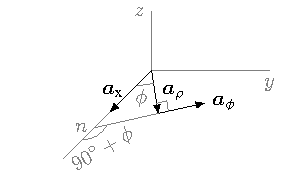
\includegraphics{figVectorDotProductUnitCartesianAndCylindrical}
\caption{کارتیسی اور نلکی اکائی سمتیات کا غیر سمتی ضرب۔}
\label{شکل_سمتیہ_غیر_سمتی_ضرب_بذریعہ_تعریف}
\end{figure}

حل:شکل \حوالہ{شکل_سمتیہ_غیر_سمتی_ضرب_بذریعہ_تعریف} میں \عددیء{\ax} اور \عددیء{\arho} کے درمیان زاویہ \عددیء{\phi} جبکہ \عددیء{\ay} اور \عددیء{\arho} کے درمیان زاویہ \عددیء{90^\circ-\phi} پایا جاتا ہے لہٰذا \عددیء{\ax \cdot \arho=\cos \phi} اور \عددیء{\ay \cdot \arho=\cos (90^\circ-\phi)=\sin \phi} کے برابر ہیں۔\عددیء{\ax} اور \عددیء{\aphi} کی سمتیں تبدیل کئے بغیر اگر انہیں یوں ہلایا جائے کہ ان کی دُم نقطہ \عددیء{n} پر آ ٹھرے تو شکل سے ظاہر ہے کہ ان کے مابین زاویہ \عددیء{90^\circ+\phi} ہے۔یوں \عددیء{\ax \cdot \aphi=\cos (90^\circ+\phi)=-\sin \phi} کے برابر ہے۔اسی طرح \عددیء{\ay} اور \عددیء{\aphi} کے درمیان \عددیء{\phi} زاویہ ہونے کی بنا پر \عددیء{\ay \cdot \aphi=\cos \phi} کے برابر ہے۔چونکہ \عددیء{\az} ان دونوں نلکی اکائی سمتیات کے عمودی ہے لہٰذا ان کا غیر سمتی ضرب صفر کے برابر ہو گا۔  
\انتہا{مثال}
%============
\begin{figure}
\centering
\begin{subfigure}{0.4\textwidth}
\centering
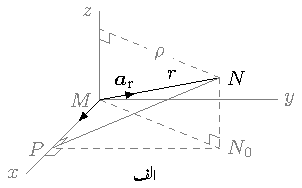
\includegraphics{figVectorSphericalUnitRadialDotWithCartesian}
\end{subfigure}%
%
\begin{subfigure}{0.4\textwidth}
\centering
\includegraphics{figVectorSphericalUnitThetaDotWithCartesian}
\end{subfigure}%
\caption{کروی اور کارتیسی اکائی سمتیات کا غیر سمتی ضرب۔}
\label{شکل_سمتیہ_کروی_کارتیسی_اکائی_غیر_سمتی_ضرب}
\end{figure}

\ابتدا{مثال}
مثال \حوالہ{مثال_سمتیہ_نلکی_کارتیسی_غیر_سمتی_اکائی_ضرب} کے طرز پر \عددیء{\ar}  کا \عددیء{\ax}، \عددیء{\ay} اور \عددیء{\az} کے ساتھ غیر سمتی ضرب حاصل کریں۔

حل: شکل \حوالہ{شکل_سمتیہ_کروی_کارتیسی_اکائی_غیر_سمتی_ضرب}-الف میں نقطہ \عددیء{N(r,\theta,\phi)} دکھایا گیا ہے جسے \عددیء{N(x,y,z)} بھی لکھا جا سکتا ہے۔شکل میں \عددیء{\ax} اور \عددیء{\ar} بھی دکھائے گئے ہیں۔شکل سے ظاہر ہے کہ \عددیء{\ax \cdot \ar=\cos \phase{NMP}} کے برابر ہے جہاں \عددیء{N} اور \عددیء{P} سے \عددیء{M} تک لکیریں کھینچنے سے زاویہ \عددیء{\phase{NMP}} بنتا ہے۔\عددیء{N} سے \عددیء{z=0} سطح پر عمود نقطہ \عددیء{N_0} دیتا ہے۔\عددیء{N_0} سے \عددیء{x} محدد پر عمود نقطہ \عددیء{P} دیتا ہے۔\عددیء{N} سے \عددیء{N_0} اور یہاں سے \عددیء{P} منتقل ہوتے ہوئے \عددیء{\ax} سمت میں کسی قسم کی حرکت نہیں کی جاتی لہٰذا اگر کارتیسی نظام میں \عددیء{N(x,y,z)} لکھا جائے تو اسی نظام میں \عددیء{N_0(x,y,0)} اور  \عددیء{P(x,0,0)} لکھے جائیں گے۔ہم \عددیء{N} سے \عددیء{x} محدد پر عمود بناتے ہوئے بھی \عددیء{P} تک پہنچ سکتے ہیں۔ تکون \عددیء{NMP} میں \عددیء{M} سے \عددیء{N} تک کا فاصلہ \عددیء{\overline{MN}=r} جبکہ \عددیء{M} سے \عددیء{P} تک کا فاصلہ \عددیء{\overline{MP}=x} اور زاویہ \عددیء{\phase{NPM}=90^\circ} ہیں لہٰذا \عددیء{\cos \phase{NMP}=\tfrac{x}{r}} ہو گا۔یہی  \عددیء{\ax} اور \عددیء{\ar} کے غیر سمتی ضرب  کے برابر ہے۔\عددیء{N} سے \عددیء{y} محدد پر عمود بناتے ہوئے یوں \عددیء{\ay \cdot \ar=\tfrac{y}{r}} اور \عددیء{N} سے \عددیء{z} محدد پر عمود سے \عددیء{\az \cdot \ar=\tfrac{z}{r}} لکھے جا سکتے ہیں۔چونکہ \عددیء{x=r\sin \theta \cos \phi}، \عددیء{y=r\sin \theta \sin \phi} اور \عددیء{z=r\cos \theta} کے برابر  ہیں لہٰذا ہم
\begin{align*}
\ar \cdot \ax&=\frac{x}{r}=\sin \theta \cos \phi\\
\ar \cdot \ay&=\frac{y}{r}=\sin \theta \sin \phi\\
\ar \cdot \az&=\frac{z}{r}=\cos \theta
\end{align*}
لکھ سکتے ہیں۔
\انتہا{مثال}
%=======================
\ابتدا{مثال}
مثال \حوالہ{مثال_سمتیہ_نلکی_کارتیسی_غیر_سمتی_اکائی_ضرب} کے طرز پر \عددیء{\atheta}  کا \عددیء{\ax} کے ساتھ غیر سمتی ضرب حاصل کریں۔

حل: شکل \حوالہ{شکل_سمتیہ_کروی_کارتیسی_اکائی_غیر_سمتی_ضرب}-ب میں نقطہ \عددیء{N} پر اکائی سمتیہ \عددیء{\atheta} جبکہ محدد کے مرکز \عددیء{M} پر \عددیء{\ax} دکھائے گئے ہیں۔\عددیء{\atheta \cdot \ax} حاصل کرنے کی خاطر سمتیات کی سمت تبدیل کئے بغیر انہیں \عددیء{z} محدد پر نقطہ \عددیء{B} منتقل کرتے ہوئے دوبارہ دکھایا گیا ہے جہاں سے واضح ہے کہ \عددیء{\atheta \cdot \ax=\cos \phase{ABC}} کے برابر ہے۔اس شکل میں \عددیء{\phase{DMC}=\phi} اور \عددیء{\phase{BMN}=\theta} کروی محدد کے زاویے ہیں۔تکون \عددیء{\Delta BMN} میں زاویہ \عددیء{\phase{MNB}} نوے درجے کا ہے۔یوں \عددیء{\phase{NBM}=90^\circ-\theta} ہو گا۔شکل سے واضح ہے کہ  \عددیء{\phase{NBM}=\phase{CBM}} ہیں۔اس طرح تکون \عددیء{\Delta BMC} میں \عددیء{\phase{BMC}=90^\circ} جبکہ \عددیء{\phase{CBM}=90^\circ-\theta} ہونے کی بنا پر \عددیء{\phase{MCB}=\theta} ہو گا۔

شکل-ب میں \عددیء{\overline{BM}=l} لیتے ہوئے تکون \عددیء{\Delta BMC}   کو دیکھتے ہوئے
\begin{align*}
\overline{BC}&=\frac{l}{\sin \theta}   \\
\overline{MC}&=\frac{l}{\tan \theta} 
\end{align*}
لکھا جا سکتا ہے۔تکون \عددیء{\Delta MDC} سے
\begin{align*}
\overline{MD}&=\overline{MC} \cos \phi=\frac{l \cos \phi}{\tan \theta} 
\end{align*} 
لکھا جا سکتا ہے۔شکل سے واضح ہے کہ \عددیء{\overline{MD}} اور \عددیء{\overline{AB}} برابر ہیں یعنی \عددیء{\overline{AB}=\overline{MD}}-یوں تکون \عددیء{\Delta BAC} سے
\begin{align*}
\cos \phase{ABC}&=\frac{\overline{AB}}{\overline{BC}}=\frac{\left(\frac{l \cos \phi}{\tan \theta}\right)}{\left(\frac{l}{\sin \theta}\right)}=\cos \theta \cos \phi
\end{align*}
حاصل ہوتا ہے۔یوں \عددیء{\ar \cdot \ax=\cos \theta \cos \phi} لکھا جا سکتا ہے۔
\انتہا{مثال}
%============

\ابتدا{مشق}
شکل \حوالہ{شکل_سمتیہ_کروی_کارتیسی_اکائی_غیر_سمتی_ضرب}-ب کے طرز پر شکل بناتے ہوئے \عددیء{\atheta \cdot \ay} اور \عددیء{\atheta \cdot \ay} حاصل کریں۔

جوابات:\عددیء{\cos \theta \sin \phi} اور \عددیء{-\sin \theta}
\انتہا{مشق}
%============

\newpage

\حصہء{سوالات}

\ابتدا{سوال}
سمتیہ \عددی{\kvec{A}=-2\ax+1\ay+7\az} اور \عددی{\kvec{B}=3\ax+5\ay-2\az} ہیں۔مندرجہ ذیل حاصل کریں: (الف) \عددی{2\kvec{A}-3\kvec{B}} اور اسی کی سمت میں اکائی سمتیہ؛ (ب) \عددی{2 \kvec{A}-5\kvec{B}+3\ax}؛ (پ) \عددی{\abs{3\kvec{A}}\abs{2\kvec{B}}(\kvec{B}-\kvec{A})}

جوابات: \عددی{-13\ax-13\ay+8\az}، \عددی{-0.648\ax-0.648\ay-0.399\az}، \عددی{28.3}، \عددی{1359\ax+1087\ay+1359\az}
\انتہا{سوال}

%=============================
\ابتدا{سوال}
نقطہ \عددی{A(1,-2,3)}، \عددی{B(3,-1,2)} اور \عددی{C(7,5,-4)} دیے گئے ہیں۔(الف) محدد کے مرکز سے \عددی{A} تک سمتیہ لکھیں؛ (ب) مرکز سے لکیر \عددی{AB} کے وسط تک سمتیہ لکھیں؛ (پ) اسی سمت میں اکائی سمتیہ لکھیں؛ (ت) تکون \عددی{ABC} کا احاطہ دریافت کریں۔

جوابات: \عددی{\ax-2\ay+3\az}، \عددی{2\ax-1.5\ay+2.5\az}، \عددی{0.566\ax-0.424\ay-0.707\az}، \عددی{23.4} 
\انتہا{سوال}
%==========================
\ابتدا{سوال}
مرکز سے نقطہ \عددیء{A} تک سمتیہ \عددیء{2\ax+\ay+3\az} ہے جبکہ مرکز سے \عددیء{\tfrac{2}{3}\ax-\tfrac{2}{3}\ay+\tfrac{1}{3}\az} اکائی سمتیہ کی سمت میں نقطہ \عددیء{B} پایا جاتا ہے۔دونوں نقطوں کے درمیان \عددیء{4} فاصلہ  ہونے کی صورت میں نقطہ \عددیء{B} دریافت کریں۔

جوابات:\عددیء{(2.57,-2.57,1.28)}
\انتہا{سوال}
%===============================
\ابتدا{سوال}
سمتی میدان \عددیء{\kvec{M}=(x+y^2)\ax+2(xy+3)\ay+4z^2\az} دیا گیا ہے۔نقطہ \عددیء{A(2,-3,1)} پر اس میدان کی قیمت حاصل کریں۔اسی نقطے پر میدان کی سمت میں اکائی سمتیہ دریافت کریں۔ایسی سطح جس پر \عددی{\abs{\kvec{M}}=5} ہو کی مساوات حاصل کریں۔اس سطح پر \عددیء{y=2} اور \عددیء{z=-1} ہونے کی صورت میں حاصل لکیر کی مساوات حاصل کریں۔

جوابات:\عددی{\kvec{M}=11\ax-6\ay+4\az}، \عددی{(0.836\ax-0.456\ay+0.304\az)}، \\ \عددی{x^2+y^2+2xy^2+4x^2y^2+24xy+16z^4-11=0}، \عددی{17x^2+56x+9=0}
\انتہا{سوال}
%===============================
\ابتدا{سوال}
سمتی میدان \عددی{\kvec{B}=2x^2\ax-3y(x+2z)\ay+5\az} اور \عددیء{\kvec{M}=(x+y+z)\ax+\tfrac{y}{x}\ay+xy\az} دیے گئے ہیں۔نقطہ \عددی{N(2,-3,-1)} پر \عددی{\kvec{B}} اور \عددیء{\kvec{M}} حاصل کریں۔اسی نقطے پر سمتیہ \عددیء{2\kvec{B}-\kvec{M}} کی سمت میں اکائی سمتیہ حاصل کریں۔

جوابات:\عددی{\kvec{B}=8\ax+5\az}، \عددی{\kvec{M}=-2\ax-1.5\ay-2\az}، \عددی{0.830\ax+0.069\ay+0.553\az}
\انتہا{سوال}
%================
\ابتدا{سوال}
 نقطہ \عددیء{N(2,-3,7))} پر میدان \عددیء{\kvec{M}=\tfrac{16}{x^2+y^2}(x\ax+y\ay)} کی سمت میں اکائی سمتیہ \عددی{\kvec{a}_M} دریافت کریں۔نقطہ \عددیء{N} پر \عددیء{\ax} اور \عددیء{\kvec{M}} کے درمیان زاویہ حاصل کریں۔اسی طرح نقطہ \عددیء{N} پر \عددیء{\ay} اور \عددیء{\kvec{M}} کے درمیان زاویہ حاصل کریں۔

جوابات:\عددی{\kvec{a}_M=0.555\ax-0.832\ay}، \عددی{56.3^{\circ}}، \عددی{33.7^{\circ}}
\انتہا{سوال}
%========================
\ابتدا{سوال}
میدان \عددیء{\kvec{M}=\tfrac{16}{x^2+y^2}(x\ax+y\ay)} کا مندرجہ ذیل دو درجی تکمل \عددی{y=3} سطح پر حاصل کریں۔
\begin{align*}
\int_{0}^{3} \int_{0}^{2} \kvec{M} \dif x \dif z\cdot \ax 
\end{align*}

جواب: \عددیء{24 \ln \frac{13}{9}}
\انتہا{سوال}
%========================
\ابتدا{سوال}
غیر سمتی ضرب استعمال کرتے ہوئے تکون \عددیء{ABC} میں زاویہ \عددی{A} اور \عددی{C} حاصل کریں۔تکون کے کونے \عددی{A(3,1,2)}، \عددی{B(4,6,2)} اور
 \عددی{C(1,4,-2)} ہیں۔

جوابات:\عددی{61.74^{\circ}} ، \عددیء{56.51^{\circ}}
\انتہا{سوال}
%===================
\ابتدا{سوال}
نقطے \عددیء{A(4,1,2)}، \عددیء{B(-2,4,3)} اور \عددیء{C(2,3,-1)} دیے گئے ہیں۔سمتیہ \عددی{\kvec{R}_{BA}} اور \عددی{\kvec{R}_{CA}} حاصل کریں۔دوسری سمتیہ  پر  پہلی سمتیہ کے \اصطلاح{عمودی سائے}\فرہنگ{عمودی سائے}\فرہنگ{سایہ!عمودی}\حاشیہب{projection}\فرہنگ{projection} کی لمبائی دریافت کریں۔لکیر \عددیء{AB} کے درمیانے نقطے سے لکیر \عددی{AC} کے درمیانے نقطے تک سیدھا سمتیہ حاصل کریں۔

جوابات: \عددی{-6\ax+3\ay+\az}، \عددی{-2\ax+2\ay-3\az}، \عددی{4.12}، \عددی{2\ax-0.5\ay-2\az}
\انتہا{سوال}
%==================
\ابتدا{سوال}
سمتیہ \عددیء{\kvec{M}=5\ax-3\ay+2\az} کا وہ حصہ حاصل کریں جو سمتیہ \عددی{\kvec{P}=-7\ax+2\ay-6\az} کے متوازی ہے۔وہ حصہ حاصل کریں جو اس کے عمودی ہے۔ 

جوابات: \عددی{4.17\ax-1.19\ay+3.57\az}، \عددی{0.83\ax-1.81\ay-1.57\az}
\انتہا{سوال}
%================
\ابتدا{سوال}
تین سمتیات \عددی{\kvec{r}_1=2\ax-1\ay+3\az}، \عددی{\kvec{r}_2=-3\ax+4\ay-5\az} اور \عددی{\kvec{r}_3=5\ax-2\ay+3\az} دیے گئے ہیں۔\عددیء{\kvec{r}_1\times \kvec{r}_2} کی سمت میں اکائی سمتیہ حاصل کریں۔ایسی اکائی سمتیہ حاصل کریں جو \عددیء{\kvec{r}_1} اور \عددیء{\kvec{r}_2} دونوں کو عمودی ہو۔سمتیہ \عددیء{\kvec{r}_2-\kvec{r}_1} اور \عددیء{\kvec{r}_2-\kvec{r}_3} دونوں کو عمودی اکائی سمتیہ حاصل کریں۔اس تکون کا رقبہ حاصل کریں جس کے اطراف \عددیء{\kvec{r}_1} اور \عددیء{\kvec{r}_2} ہوں۔اس تکون کا رقبہ حاصل کریں جس کے کونے یہ تین سمتیات دیتے ہیں۔ 

جوابات:\عددی{-0.81\ax+0.16\ay+0.58\az}، \عددی{\mp(-0.81\ax+0.16\ay+0.58\az)}، \عددی{\mp(0.29\ax+0.88\ay+0.37\az)}، \عددی{4.3}، \عددی{13.6}
\انتہا{سوال}
%===============
\ابتدا{سوال}
نقطہ \عددی{N(5,10,4)} پر سمتیات \عددیء{\kvec{R}_{AN}=-3\ax+6\ay+12\az} اور \عددیء{\kvec{R}_{BN}=12\ax+20\ay-5\az} مل کر تکون بناتی ہیں۔تکون کی عمودی اکائی سمتیہ حاصل کریں۔سمتیہ \عددی{\kvec{R}_{BN}} کے عمودی اور تکون کی سطح کے متوازی اکائی سمتیہ حاصل کریں۔تکون کی سطح پر اس اکائی سمتیہ کو حاصل کریں جو نقطہ \عددیء{N} پر تکون کے کونے کو نصف زاویہ میں کاٹے۔

جوابات:\عددی{\mp(-0.83\ax+0.39\ay-0.40\az)}، \عددی{\mp(0.26\ax-0.38\ay-0.89\az)}، \عددی{0.19\ax+0.87\ay+0.45\az}
\انتہا{سوال}
%=============
\ابتدا{سوال}
سمتیہ \عددی{\kvec{M}=(x^2+y^2)^{-1}(x\ax+y\ay)} کو نلکی محدد کے متغیرات میں لکھیں۔نقطہ \عددیء{(5,30^{\circ},6)} پر سمتیہ کی قیمت کارتیسی اور نلکی محدد میں حاصل کریں۔

جوابات:\عددی{\kvec{M}=\tfrac{1}{\rho}\arho}، \عددیء{\kvec{M}=0.41\ax+0.29\ay}، \عددی{\kvec{M}=\tfrac{1}{5}\arho}
\انتہا{سوال}
%===============
\ابتدا{سوال}
نقطہ \عددی{N(\rho=2,\phi=45^{\circ},z=12)} اور \عددیء{P(\rho=5,\phi=-60^{\circ},z=-6)} دئے گئے ہیں۔کارتیسی محدد میں، پہلے نقطے سے دوسرے نقطے کی جانب اکائی سمتیہ حاصل کریں۔اسی اکائی سمتیہ کو پہلے نقطے پر پائے جانے والے نلکی محدد کے متغیرات کی صورت میں لکھیں۔اسی اکائی سمتیہ کو دوسرے نقطے پر پائے جانے والے نلکی محدد کے متغیرات کی صورت میں لکھیں۔

جوابات: \عددی{0.057\ax-0.303\ay-0.951\az}، \عددی{-0.174\arho-0.255\aphi-0.951\az}، \عددی{0.292\arho-0.180\aphi-0.951\az}
\انتہا{سوال}
%================
\ابتدا{سوال}
نقطہ \عددیء{N(\rho=5,\phi=30^{\circ},z=6)} سے نقطہ \عددی{P(\rho=10,\phi=75^{\circ},z=12)} تک سمتیہ کارتیسی محدد میں لکھیں۔اسی سمت میں اکائی سمتیہ بھی لکھیں۔کارتیسی محدد میں دوسرے نقطے سے مرکز تک اکائی سمتیہ لکھیں۔

جوابات:\عددی{-1.74\ax+7.16\ay+6\az}، \عددیء{-0.183\ax-0.618\ay+0.631\az}، \عددی{0.166\ax-0.618\ay-0.768\az}
\انتہا{سوال}
%================
\ابتدا{سوال}
نقطہ \عددی{M(5,-3,2)} سے نقطہ \عددیء{N(10,2,-5)} تک سمتیہ کو نقطہ \عددی{M} پر نلکی محدد کے اکائی سمتیات کی مدد سے لکھیں۔دوسرے نقطے سے پہلے نقطے کی سمت میں اکائی سمتیہ کو دوسرے  نقطے پر نلکی اکائی سمتیات کی مدد سے لکھیں۔دوسرے نقطے سے مرکز تک اکائی سمتیہ دوسرے نقطے کے اکائی سمتیات کی صورت  میں لکھیں۔ 

جوابات: \عددی{-1.71\arho-6.86\aphi+7\az}، \عددی{0.59\arho+0.39\aphi-0.7\az}، \عددی{0.90\arho+0.44\az} 
\انتہا{سوال}
%================
\ابتدا{سوال}
رداس \عددی{\rho=2} اور \عددیء{\rho=6} حجم گھیرتے ہیں جو \عددی{z=11} تا \عددیء{z=13} اور \عددی{\phi=30^{\circ}} تا \عددی{\phi=60^{\circ}} پایا جاتا ہے۔اس جسم کے حجم کو تین درجی تکمل سے حاصل کریں۔اس کی بھی تکمل سے سطح بھی حاصل کریں۔

جوابات: \عددی{16.8}، \عددی{41.1}
\انتہا{سوال}
%==================
\ابتدا{سوال}
نقطہ \عددیء{N(5,3,8)} سے نقطہ \عددی{P(3,-4,2)} تک سمتیہ کارتیسی، نلکی اور کروی محدد میں حاصل کریں۔پہلے نقطے کے اکائی سمتیات استعمال کریں۔تینوں سمتیات کی لمبائی حاصل کرتے ہوئے ثابت کریں کہ تینوں سمتیات کی لمبائی برابر ہے۔

جوابات:\عددی{-2\ax-7\ay-6\az}، \عددی{-5.3165\arho-4.9735\aphi-6.0000\az}، \\
 \عددی{  -8.6615\ar-2.7739\atheta-2.5069\aphi}، \عددی{9.434}
\انتہا{سوال}
%==================
\ابتدا{سوال}
نقطہ \عددی{N} پر سمتیہ \عددی{\kvec{K}=3\ar-2\atheta+8\aphi} اور \عددی{\kvec{G}=2\ar+5\atheta+2\aphi} دیے گئے ہیں۔ان کی غیر سمتی ضرب \عددی{\kvec{K}\cdot\kvec{G}} حاصل کریں۔دوسری سمتیہ کی پہلی سمتیہ کی سمت میں لمبائی حاصل کریں۔پہلی سمتیہ کا وہ حصہ دریافت کریں جو دوسری سمتیہ کی سمت میں ہے۔دونوں سمتیوں کا سمتی ضرب \عددی{\kvec{K} \times \kvec{G}} حاصل کریں۔اس نقطے پر دونوں سمتیوں کی عمودی اکائی سمتیہ حاصل کریں۔

جوابات:\عددی{12}، \عددی{1.3675}، \عددی{0.46753\ar-0.31169\atheta+1.24675\aphi}، \عددی{  44\ar-10\atheta-19\aphi}،\\ \عددی{\mp(  0.89871\ar-0.20425\atheta-0.38808\aphi)}
\انتہا{سوال}
%=====================
\ابتدا{سوال}
ایک جسم \عددی{r=6} تا \عددی{r=10}، \عددی{\theta=30^{\circ}} تا \عددی{\theta=70^{\circ}} اور \عددی{\phi=25^{\circ}} تا \عددی{\phi=100^{\circ}} حجم گھیرتا ہے۔اس جسم کے دو دور ترین کونوں کے درمیان فاصل حاصل کریں۔جسم کی سطح کا رقبے حاصل کریں۔جسم کی حجم دریافت کریں۔

جوابات:\عددی{9.27}، \عددی{198.27}، \عددی{179.25}
\انتہا{سوال}
%====================
\ابتدا{سوال}
نقطہ \عددی{N(5,4,-2)} اور \عددی{P(6,4,10)} دیے گئے ہیں۔پہلے نقطے کو نلکی محدد میں لکھیں۔پہلے نقطے کے متغیرات استعمال کرتے ہوئے پہلے نقطے سے دوسرے نقطے تک سمتیہ نلکی محدد میں لکھیں۔

جوابات:\عددی{P(6.4031,38.6598^{\circ},-2.0000)}، \عددی{  0.57\arho-0.82\aphi+12\az}
\انتہا{سوال}
%==================
